\chapter{Experimentos e resultados}
\label{chap:Experimentos e resultados}
\lettrine{N}{este} capítulo presentaranse os experimentos realizados e os resultados obtidos.
Para iso, comezarase presentando unha vista xeral do proceso de experimentación, 
seguido dos propios experimentos realizados, para finalmente analizar os resultados obtidos en conxunto e as conclusións que se poden extraer deles.

\section{Vista Xeral}
\label{sec:Vista Xeral}

O obxectivo do traballo é determinar se as redes implícitas son aptas para a tarefa de rexistro de retinas. A comparación principal céntrase na función de activación empregada (SIREN ou ReLU), sobre os datases FIRE e RFMID.

A avaliación inicial sobre o dataset FIRE, como se pode ver nas figuras \ref{fig:FIRE_relu} e \ref{fig:FIRE_SIREN}, amosou un rendemento limitado. A categoría P resultou imposible de rexistrar, probablemente debido ao baixo grao de superposición entre as imaxes (<75\%), mentres que as categorías S e A apenas acadaron taxas de éxito do 20\%.

Co obxectivo de mellorar este rendemento e comprender os factores clave que inflúen no rexistro, deseñouse unha serie de experimentos sistemáticos. Esta sección ofrece unha panorámica de cada un destes experimentos, adiantando a súa motivación e os seus achados principais, que serán detallados no resto do capítulo.

\begin{itemize}
\item \textbf{Función de perda:} A motivación era atopar a métrica de similitude máis robusta para as imaxes de retina, que presentan gran variabilidade en contraste e iluminación. O principal achado foi que a elección óptima depende da natureza das imaxes: para imaxes reais con variabilidade (FIRE), as funcións baseadas en características estruturais como NCC ofreceron os mellores resultados; para imaxes sintéticas sen dita variabilidade (RFMID), as funcións baseadas en píxeles como L1 foron superiores.

\item \textbf{Resolución da imaxe:} Investigouse se a alta resolución das imaxes de retina (ata 2160x2160) aportaba un beneficio significativo fronte ao custo computacional. A conclusión foi que, aínda que resolucións moi baixas eran insuficientes, non se observou unha mellora notable por enriba de 1250x1250 píxeles, establecendo este valor como un bo equilibrio entre detalle e eficiencia.

\item \textbf{Regularización:} Este experimento foi crucial para evitar as deformacións non realistas, un risco particular nos modelos SIREN debido ao seu sesgo cara ás altas frecuencias. Confirmouse que certo grao de regularización é indispensable, mais a cantidade óptima de regularización non é universal, senón que depende da complexidade da transformación.

\item \textbf{Tamaño de lote:} A análise cualitativa suxería que este era un parámetro de gran impacto. Os experimentos confirmaron que o é un dos factores máis críticos para o éxito do rexistro. Un tamaño de lote grande (e.g., 10000 ou máis) é fundamental para obter bos resultados.

\item \textbf{Estratexias de mostraxe:} A hipótese inicial era que priorizar rexións con máis información (vasos sanguíneos, disco óptico) mediante estratexias de mostraxe "intelixentes" melloraría o rendemento. Os resultados demostraron que ningunha das estratexias propostas (uniforme, ponderada) ofreceu unha vantaxe significativa sobre a mostraxe aleatoria tradicional.

\item \textbf{Inicialización:} Dada a natureza non convexa do problema de optimización, explorouse se unha selección coidadosa dos pesos iniciais podería mellorar a converxencia. Implementouse unha "lotería de inicialización" que escolle a mellor de varias execucións iniciais. Observouse unha mellora marxinal pero consistente, indicando que a inicialización ten un certo impacto, aínda que non é un factor transformador.

\item \textbf{Axuste dinámico do tamaño de lote:} Probouse a estratexia de comezar cun tamaño de lote pequeno para aprender a transformación global e logo aumentalo para refinar detalles locais. O resultado foi concluínte e contrario á hipótese: esta estratexia resultou ser prexudicial, empeorando o rendemento. Un tamaño de lote grande e constante dende o inicio demostrou ser máis eficaz.

\end{itemize}

A menos que se especifique o contrario, para os experimentos utilizarase un learning rate de 0.0001, tamaño de lote de 10000 puntos e 1500 épocas. Estes valores determináronse a partir dos utilizados orixinalmente por IDIR e da análise cualitativa dos resultados obtidos en experimentos preliminares. O conxunto destes experimentos permite construír unha comprensión detallada das fortalezas e debilidades das redes implícitas nesta tarefa.
\begin{figure}[tbp]
    \centering
    \begin{subfigure}[b]{0.5\textwidth}
        \centering
        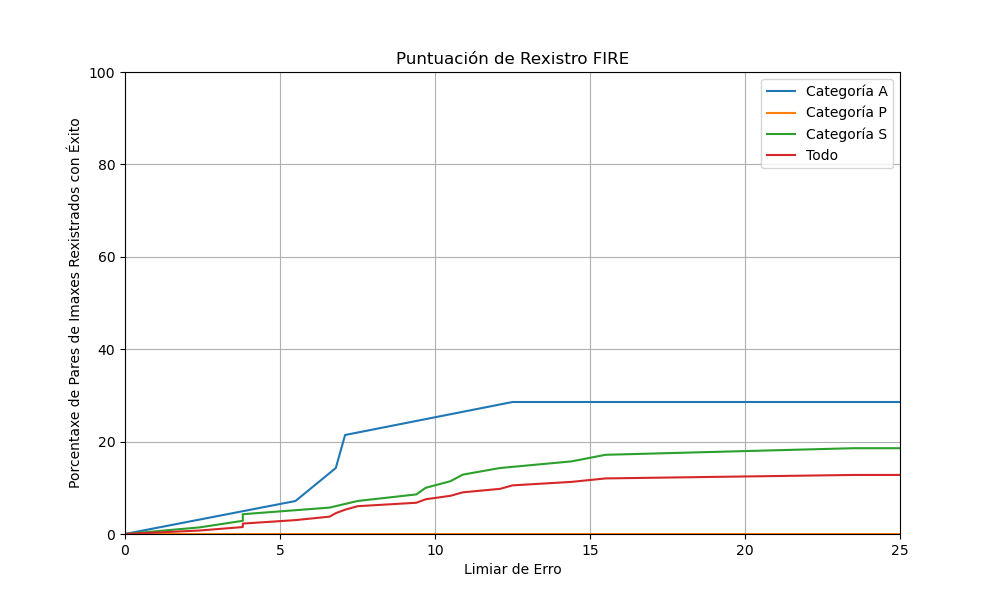
\includegraphics[width=\textwidth]{imaxes/FIRE_scores/fire_registration_score_ReLU.png}
        \caption{Métrica FIRE ca función de activación ReLU}
        \label{fig:FIRE_relu}
    \end{subfigure}\hfill
    \begin{subfigure}[b]{0.5\textwidth}
        \centering
        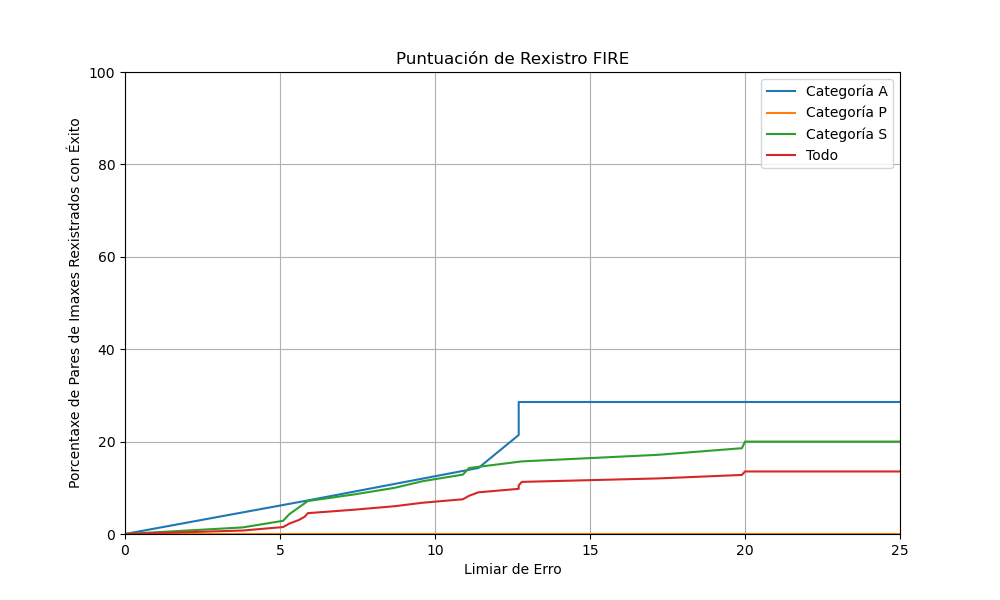
\includegraphics[width=\textwidth]{imaxes/FIRE_scores/fire_registration_scores_SIREN.png}
        \caption{Métrica FIRE ca función de activación SIREN}
        \label{fig:FIRE_SIREN}
    \end{subfigure}
    \caption{Métricas dataset FIRE}
    \label{fig:FIRE_scores}
\end{figure}

\subsection{Descripción dos experimentos}
\label{subsec:Descripción dos experimentos}

% Os experimentos realizados divídense en varias categorías, cada unha coa súa motivación específica:

\textbf{Experimentos iniciais:} Nesta parte realizaranse experimentos para determinar uns valores aceptables para os parámetros da rede no contexto da imaxe oftalmolóxica, 
así como determinar a súa influenza no rendemento da rede.

\begin{itemize}
    \item \textbf{Función de perda:} Debido ás características únicas das imaxes de retina, con variabilidade en iluminación e contraste, é crucial determinar que función de perda é máis robusta para esta tarefa. Comparáronse funcións baseadas en píxeles (MSE, L1) con funcións baseadas en características estruturais (NCC, SSIM) para determinar cal captura mellor as correspondencias entre imaxes retinianas.
    \item \textbf{Resolución da imaxe:} As imaxes de retina poden ter resolucións de ata 2160×2160 píxeles, significativamente maiores que as imaxes de pulmón utilizadas orixinalmente por IDIR (512×512). É necesario determinar se unha maior resolución mellora o rendemento ou se introduce ruído que perxudica o rexistro.
    \item \textbf{Regularización:} SIREN ten un sesgo inherente cara sinais de alta frecuencia, o que pode provocar sobreaxuste. Avalíase o impacto de diferentes termos de regularización (jacobiana, hiperelástica, enerxía de flexión) para determinar os valores óptimos que eviten deformacións non realistas.
    \item \textbf{Tamaño de lote:} A densidade de puntos mostrados á rede pode ser crucial para o éxito do rexistro. Batch sizes maiores proporcionan máis información por iteración, pero a un maior custo computacional. Investígase o equilibrio óptimo entre eficiencia e rendemento.
\end{itemize}

\textbf{Estratexias de mostraxe:} As imaxes de retina teñen zonas con diferentes cantidades de información estrutural (vasos sanguíneos, disco óptico vs. fondo uniforme). Compáranse estratexias de mostraxe aleatorio, uniforme e ponderado por contido para determinar se priorizar certas rexións mellora o rexistro.

\textbf{Inicialización:} A natureza non convexa da función de perda pode facer que diferentes inicializacións converxan a mínimos locais distintos. Implementouse unha lotería de inicialización para seleccionar a inicialización máis prometedora baseándose na perda inicial.

\textbf{Axuste dinámico do tamaño de lote:} Teorízase que a rede podería beneficiarse de aprender primeiro transformacións globais con batch sizes pequenos e despois refinar con batch sizes maiores para capturar detalles locais.

% \section{Experimentos iniciais}
% \label{sec:Experimentos iniciais}

% % Inicialmente tentaremos determinar uns valores aceptables para varios dos parámetros da rede.
% % Isto é relevante xa que moitos destes parámetros son dependentes uns de outros.
% Nesta sección realizaranse experimentos para determinar uns valores aceptables para os parámetros da rede no contexto da imaxe oftalmolóxica, 
% así como determinar a súa influenza no rendemento da rede.

\section{Exemplos de rexistro}
\label{sec:Exemplos de rexistro}

Diferentes exemplos de rexistro, tanto exitosos como fallidos, pódense observar na figura \ref{fig:reg_examples}.
A primeira imaxe corresponde ca imaxe fixa, a segunda corresponde ca imaxe rexistrada, a terceira ca imaxe móbil e a cuarta o campo de deformación aplicado a unha grella cadrada.
 
Pódense observar os puntos de control, sendo os brancos os da imaxe fixa, os verdes os da imaxe móbil e os azuis os desprazados pola rede.
\begin{figure}[tbp]
    \centering
    \begin{subfigure}[b]{0.45\textwidth}
        \centering
        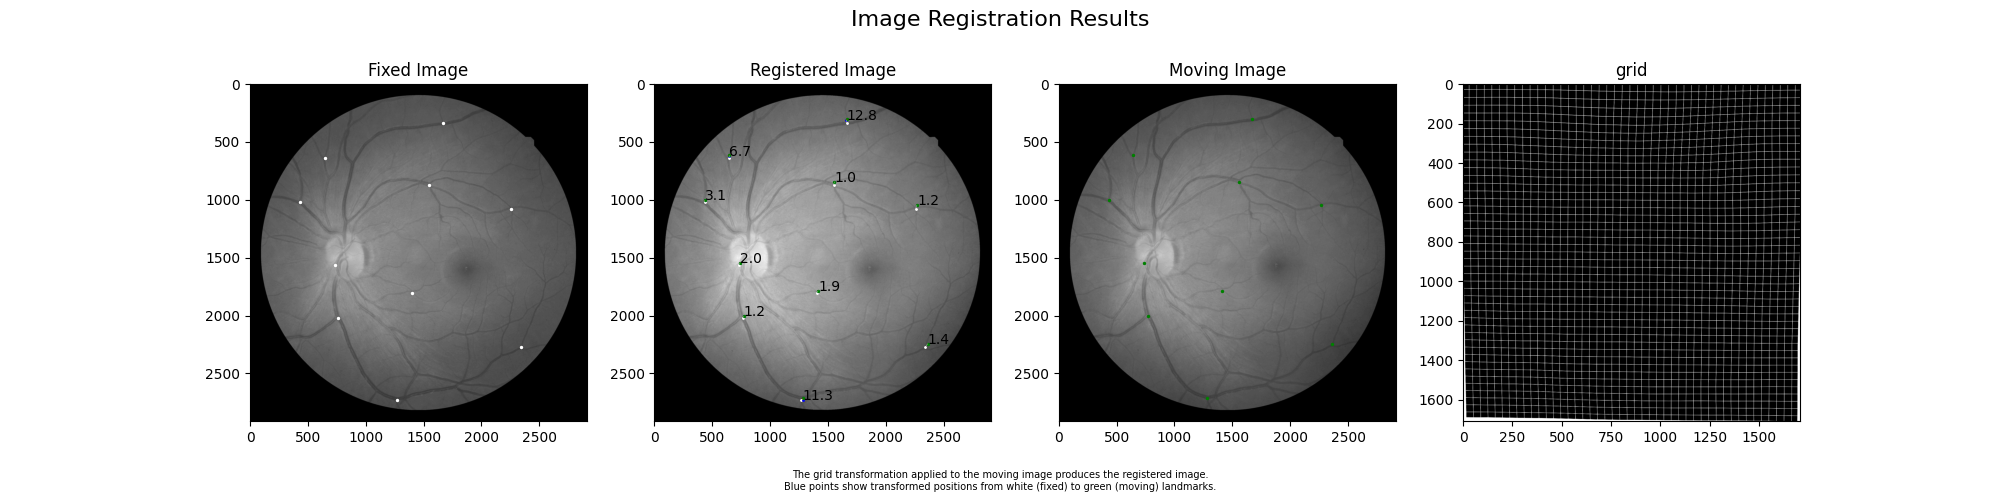
\includegraphics[width=\textwidth]{imaxes/reg_examples/FIRE_MLP_buena.png}
        \caption{Rexistro exitoso dunha parella de imaxes do dataset FIRE ca función de activación ReLU}
        \label{fig:reg_example_FIRE_MLP_buena}
    \end{subfigure}\hfill
    \begin{subfigure}[b]{0.45\textwidth}
        \centering
        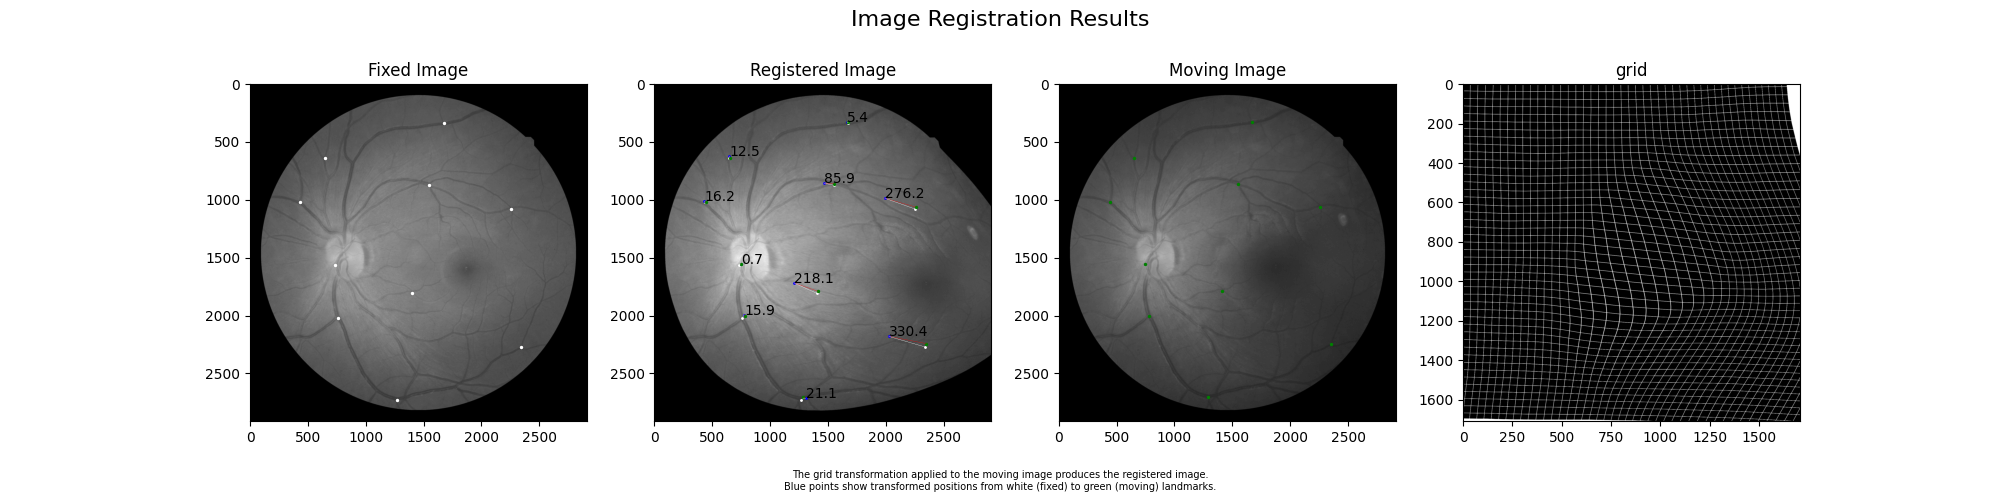
\includegraphics[width=\textwidth]{imaxes/reg_examples/FIRE_MLP_mala.png}
        \caption{Rexistro fallido dunha parella de imaxes do dataset FIRE ca función de activación ReLU}
        \label{fig:reg_example_FIRE_MLP_mala}
    \end{subfigure}

    \vskip\baselineskip

    \begin{subfigure}[b]{0.45\textwidth}
        \centering
        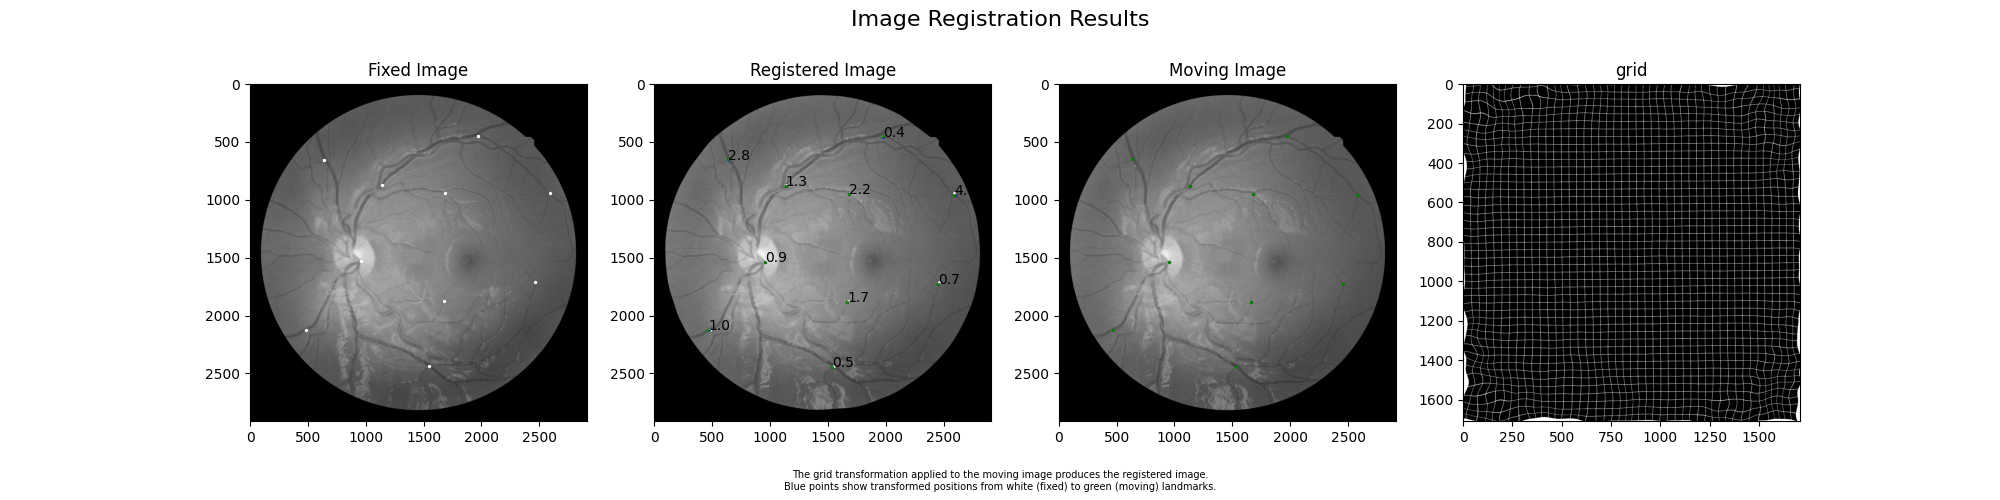
\includegraphics[width=\textwidth]{imaxes/reg_examples/FIRE_SIREN_buena.png}
        \caption{Rexistro exitoso dunha parella de imaxes do dataset FIRE ca función de activación SIREN}
        \label{fig:reg_example_FIRE_SIREN_buena}
    \end{subfigure}\hfill
    \begin{subfigure}[b]{0.45\textwidth}
        \centering
        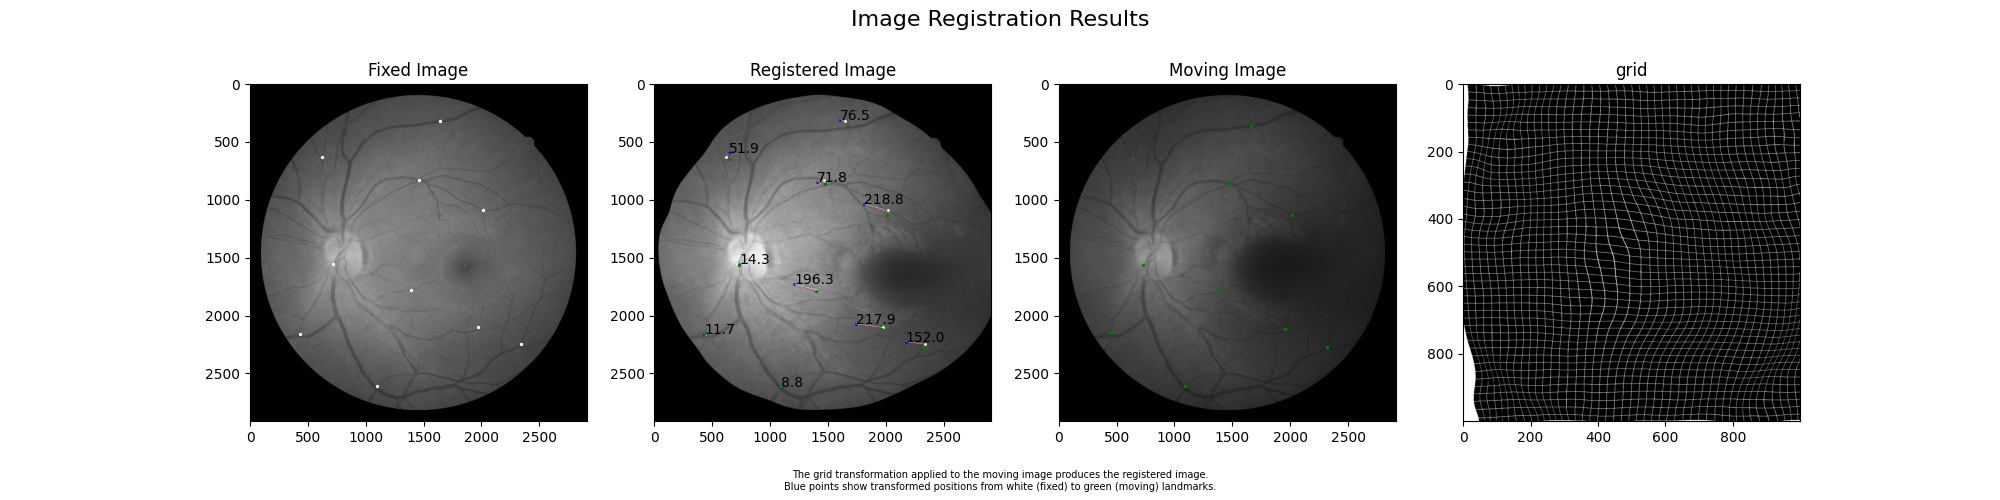
\includegraphics[width=\textwidth]{imaxes/reg_examples/FIRE_SIREN_mala.png}
        \caption{Rexistro fallido dunha parella de imaxes do dataset FIRE ca función de activación SIREN}
        \label{fig:reg_example_FIRE_SIREN_mala}
    \end{subfigure}

    \vskip\baselineskip

    \begin{subfigure}[b]{0.45\textwidth}
        \centering
        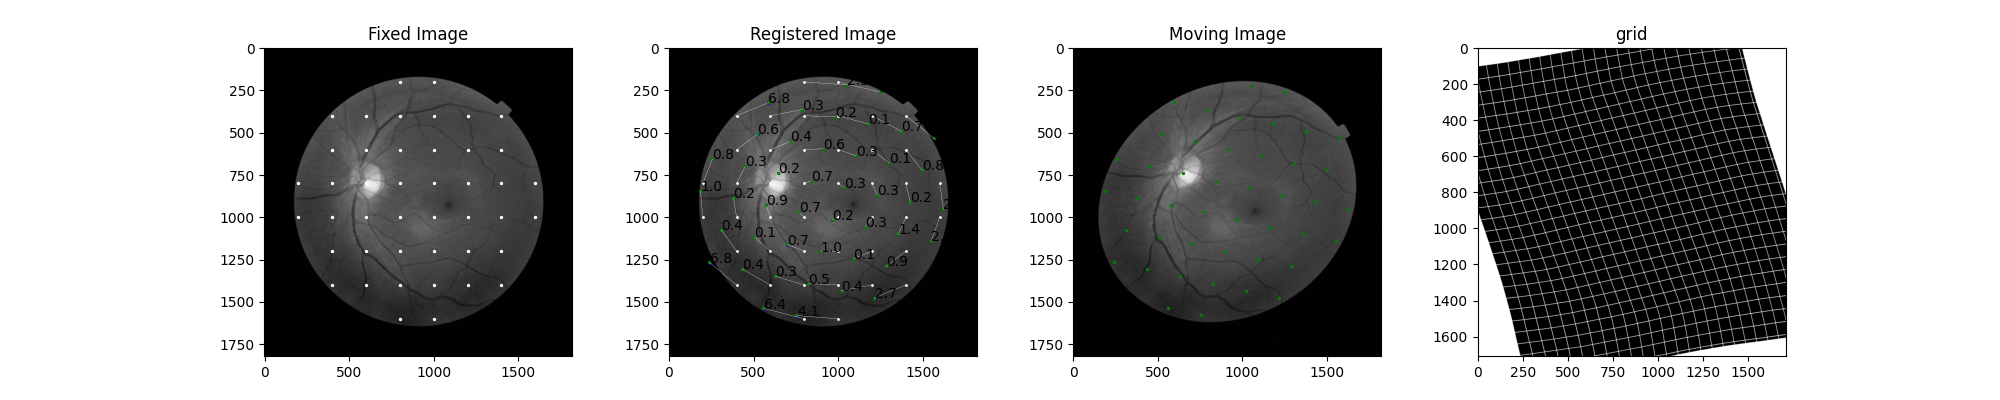
\includegraphics[width=\textwidth]{imaxes/reg_examples/RFMID_MLP_buena.png}
        \caption{Rexistro exitoso dunha parella de imaxes do dataset RFMID ca función de activación ReLU}
        \label{fig:reg_example_RFMID_MLP_buena}
    \end{subfigure}\hfill
    \begin{subfigure}[b]{0.45\textwidth}
        \centering
        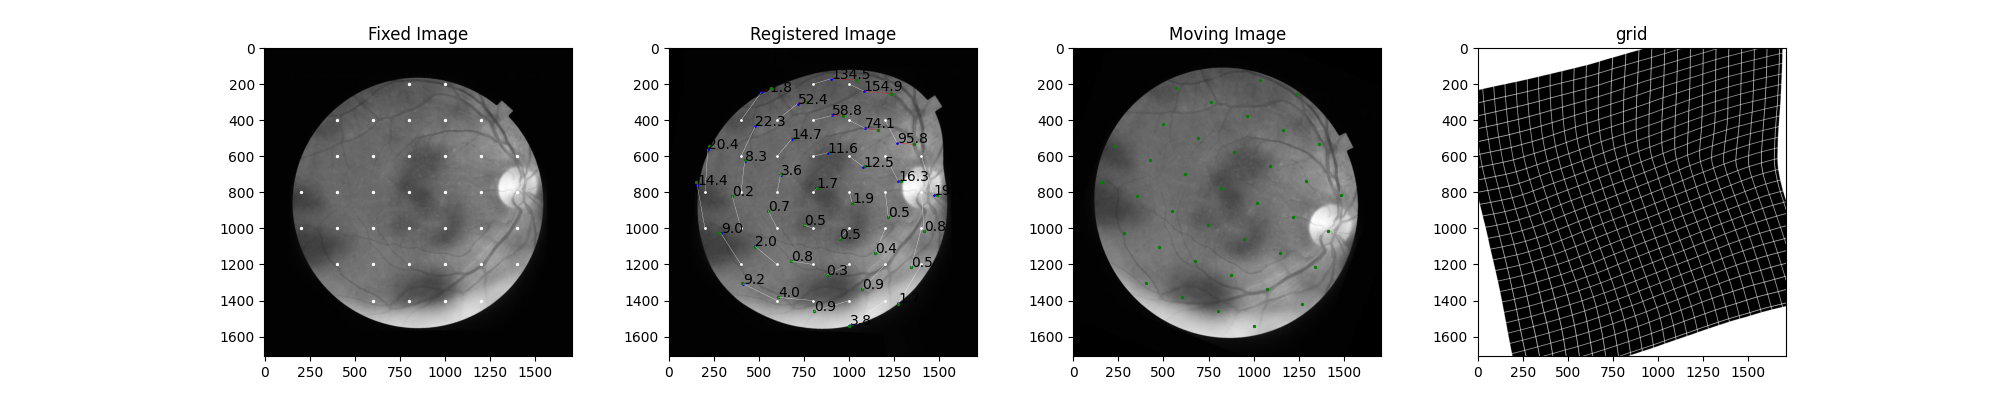
\includegraphics[width=\textwidth]{imaxes/reg_examples/RFMID_MLP_mala.png}
        \caption{Rexistro fallido dunha parella de imaxes do dataset RFMID ca función de activación ReLU}
        \label{fig:reg_example_RFMID_MLP_mala}
    \end{subfigure}

    \vskip\baselineskip

    \begin{subfigure}[b]{0.45\textwidth}
        \centering
        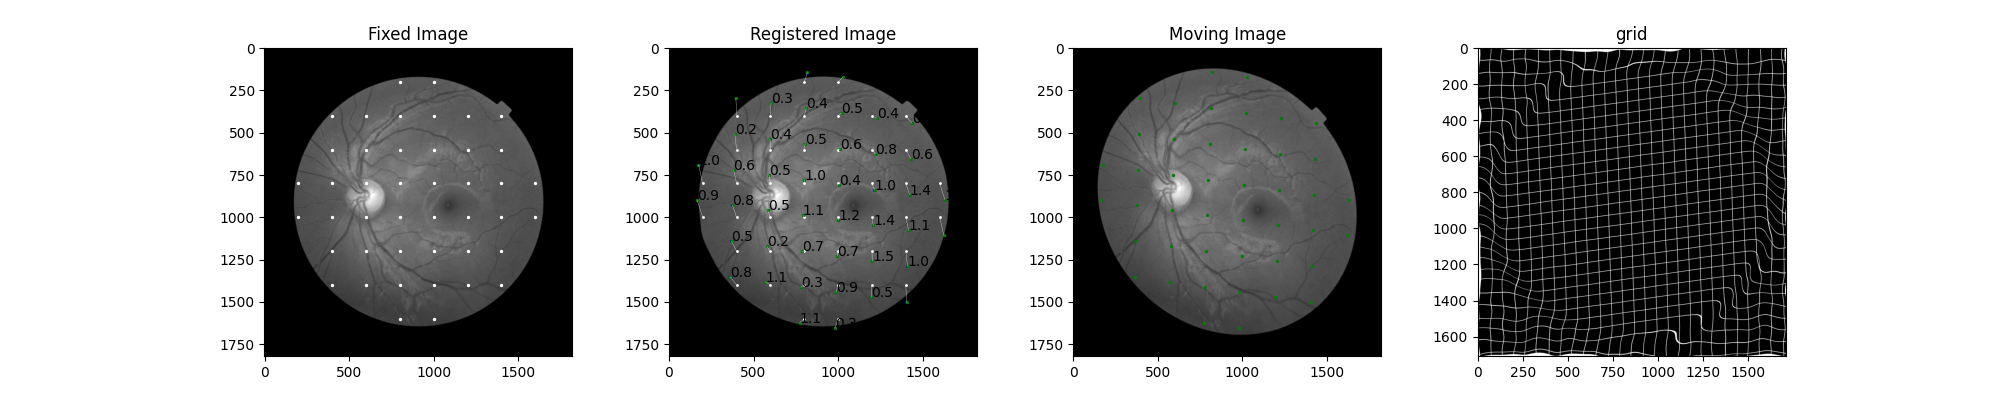
\includegraphics[width=\textwidth]{imaxes/reg_examples/RFMID_SIREN_buena.png}
        \caption{Rexistro exitoso dunha parella de imaxes do dataset RFMID ca función de activación SIREN}
        \label{fig:reg_example_RFMID_SIREN_buena}
    \end{subfigure}\hfill
    \begin{subfigure}[b]{0.45\textwidth}
        \centering
        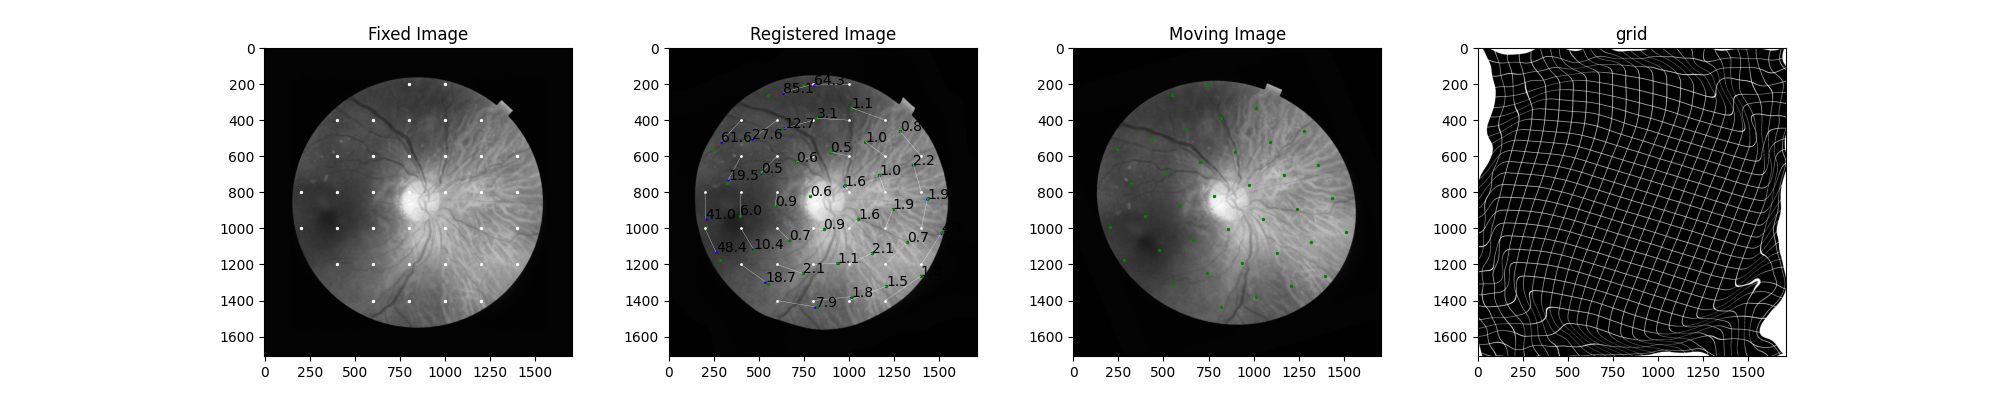
\includegraphics[width=\textwidth]{imaxes/reg_examples/RFMID_SIREN_mala.png}
        \caption{Rexistro fallido dunha parella de imaxes do dataset RFMID ca función de activación SIREN}
        \label{fig:reg_example_RFMID_SIREN_mala}
    \end{subfigure}

    \caption{Exemplos de rexistro: combinacións de dataset (FIRE/RFMID), función de activación (relu/SIREN) e éxito.}
    \label{fig:reg_examples}
\end{figure}

\section{Función de perda}
\label{sec:Función de perda}

\subsection{Planteamento}
\label{subsec:Planteamento-perda}

% A función de loss é un dos aspectos máis importantes á hora de entrenar unha rede neuronal.
As funcións de perda valoradas para este traballo xa forón explicadas na sección \ref{subsubsec:Termos de Perda}.

Para determinar cal é a función de perda mais adecuada para a tarefa de rexistro de retinas, realizáronse experimentos comparando o rendemento de cada unha sobre unha mostra de imaxes dos datases de FIRE e RFMID.
Xa que a rede non é capaz de rexistrar con éxito a gran parte das imaxes nestas condicións, tomaráse a distancia media de todos os puntos como métrica de comparación.

\subsection{Resultados}
\label{subsec:Resultados-perda}

Presentase na figura \ref{fig:loss_functions_comparison} a comparación entre as diferentes funcións de perda.

% : \ref{tab:mean_distances_resolution}, 

% \begin{table}[h]
%     \centering
%     \begin{tabular}{|l|c|c|}
%     \hline
%     Loss Function & FIRE Mean Distance & RFMID Mean Distance \\ \hline
%     ncc & 250.59 & 36.04 \\ \hline
%     mse & 392.94 & 9.50 \\ \hline
%     l1 & 404.83 & 5.42 \\ \hline
%     smoothl1 & 414.79 & 7.01 \\ \hline
%     \end{tabular}
%     \caption{Distancias medias según a función de perda. Valores máis baixos son mellores.}
%     \label{tab:mean_distances}
% \end{table}


% \begin{table}[ht]
%     \centering
%     \begin{tabular}{|l|cc|cc|}
%     \hline
%     \multirow{2}{*}{Loss Function} & \multicolumn{2}{c|}{FIRE Dataset} & \multicolumn{2}{c|}{RFMID Dataset} \\ \cline{2-5}
%      & Relu & SIREN & Relu & SIREN \\ \hline
%     huber & 399.86 & 397.45 & 7.13 & 57.31 \\ \hline
%     l1 & 404.83 & 391.87 & 5.42 & 52.91 \\ \hline
%     mse & 392.94 & 410.97 & 9.50 & 121.54 \\ \hline
%     ncc & 250.59 & 281.03 & 36.04 & 79.84 \\ \hline
%     smoothl1 & 414.79 & 387.71 & 7.01 & 60.74 \\ \hline
%     ssim & 268.72 & 264.98 & 23.34 & 55.07 \\ \hline
%     \end{tabular}
%     \caption{Distancias medias segundo función de perda, tipo de rede e datasets (FIRE vs. RFMID)}
%     \label{tab:mean_distances}
%     % \hyperlink{tableRefTarget}{Volver ao texto de referencia}
% \end{table}

\begin{figure}[tbp]
    \centering
    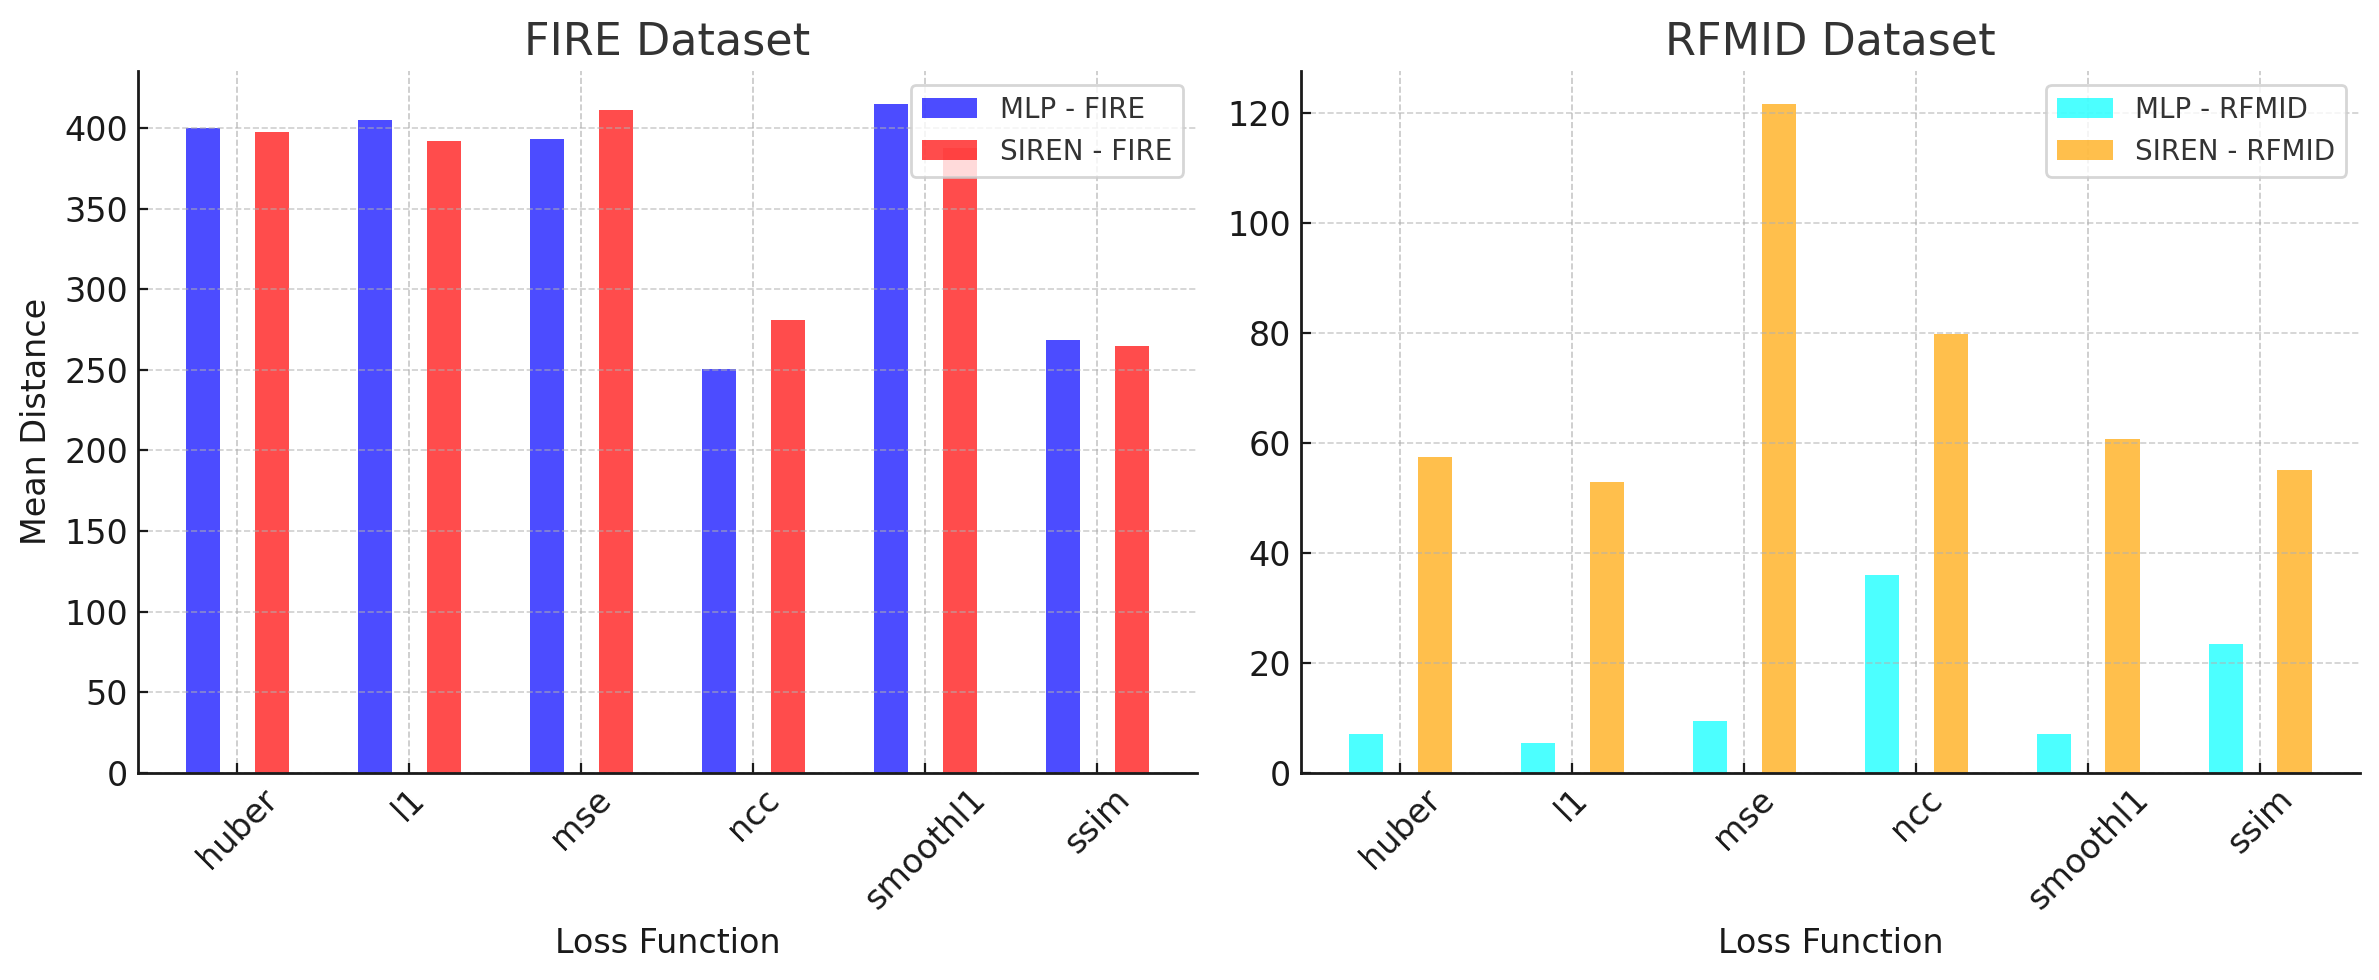
\includegraphics[width=1\textwidth]{imaxes/losstype.png}
    \caption{Comparación de diferentes funcións de perda sobre imaxes de FIRE e RFMID}
    \label{fig:loss_functions_comparison}
\end{figure}

\subsection{Discusión}
\label{subsec:Discusion-loss}

Obsérvase como as métricas que teñen en conta a estructura da imaxe (NCC, SSIM) tenden a dar mellores resultados que aquelas que non o fan (MSE, Huber, Smooth L1) co dataset de FIRE, mentres que con RFMID ocurre ó contrario.
Isto pode deberse a que as imaxes reais de retina teñen unha maior variabilidade na iluminación e contraste, polo que as métricas que non teñen en conta a estructura da imaxe serán menos robustas a estas diferenzas.
No caso de RFMID, ao ser imaxes sintéticas, a variabilidade na iluminación e contraste é nula, o que explica os mellores resultados das métricas que non teñen en conta a estructura da imaxe.
Da mesma forma, a función de activación Relu tende a producir funcións predominantemente lineares, o que se adapta mellor ás transformacións realizadas no dataset RFMID.

SSIM é menos robusta ao ruído e sensible o tamaño das seccións utilizadas, así como computacionalmente mais costosa. Ademais, ten outro custo engadido xa que non é posible calcular SSIM tan só comparando os puntos mostrados xa que utiliza xanelas deslizantes para evaluar luminancia, contraste e estrutura. 
Para utilizala é necesario reconstruir a imaxen en cada iteracion o que ten un alto custo computacional.
No caso de non reconstruir a imaxe e utilizar os puntos mostrados directamente, esta métrica funciona igualmente mais con resultados lixeiramente peores, xa que perde toda a súa capacidade de capturar variacións locais de luminancia, contraste e estrutura, o que se tradúce nunha función de perda global sen consideraciós locais.

\subsection{Conclusións}
\label{subsec:Conclusions-loss}

En base aos resultados obtidos, pódense extraer as seguintes conclusións:
\begin{itemize}
    \item Para o dataset FIRE, que contén imaxes reais de retina con variabilidade en iluminación e contraste, as funcións de perda baseadas en características estruturais como NCC e SSIM proporcionan resultados significativamente mellores.
    \item Para o dataset RFMID, que contén imaxes con tan só variación xeométrica, as funcións de perda baseadas en píxeles como L1 e Huber ofrecen mellores resultados.
    \item Obsérvase unha diferenza sistemática entre os modelos Relu e SIREN, sendo os primeiros máis efectivos para o dataset RFMID, mentres que ambos mostran rendementos comparables para FIRE.
\end{itemize}
% 4. SSIM, a pesar de ser teoricamente robusta a cambios locais, non mostra unha vantaxe significativa sobre NCC.

% A elección de NCC como función de perda estándar baséase tanto na súa robustez empírica coma na súa consistencia co obxectivo de alinear imaxes reais de retina, onde a variabilidade en iluminación e contraste é un factor importante.

\section{Resolución da imaxe}
\label{sec:Resolución da imaxe}

\subsection{Planteamento}
\label{subsec:Planteamento-resolution}

Para determinar cal é a resolución mais adecuada, realizáronse experimentos comparando o rendemento de cada unha sobre unha mostra de imaxes dos datases de FIRE e RFMID.
Debido a que a rede non é capaz de rexistrar con éxito a gran parte das imaxes, tomaráse a distancia media de todos os puntos como métrica de comparación.

A resolución da imaxe inflúe de forma directa no resto de parámetros da rede.
Por exemplo, un tamaño de lote de 1000 puntos nunha imaxe de 256x256 é unha densidade de puntos moito maior que nunha imaxe de 1024x1024.

Ademais, a resolución da imaxe tamén inflúe na capacidade da rede para aprender as transformacións, xa que a información que recibe é mais detallada. 
Isto pode ser beneficioso se estos detalles conteñen información relevante para a tarefa de rexistro, pero tamén podería ser perxudicial se conteñen unha gran parte de ruido.

O tamaño das imaxes tamén é unha das principais diferencias entre as imaxes de retina e as de pulmóns utilizadas orixinalmente por IDIR, tendo estas últimas de 512x512 mentres que as imaxes dos ollos contan con resolucións de ata 2160x2160.

\subsection{Resultados}
\label{subsec:Resultados-resolution}

% \ref{tab:mlp_mean_distances_fire}, \ref{tab:siren_mean_distances_fire}, \ref{tab:mlp_mean_distances_rfmid}, \ref{tab:siren_mean_distances_rfmid}
% \ref{tab:mean_distances_resolution}
Preséntase na figura \ref{fig:resoluciónchart} a comparación entre as diferentes resolucións.

\begin{figure}[tbp]
    \centering
    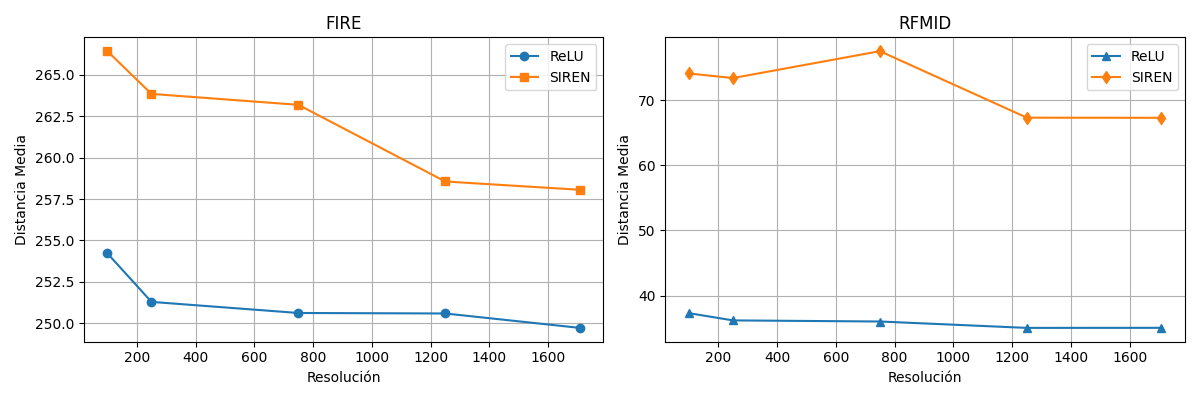
\includegraphics[width=1\textwidth]{imaxes/resolutionchart.png}
    \caption{Comparación de diferentes resolucións de perda sobre imaxes de FIRE e RFMID. Menor distancia media é mellor.}
    \label{fig:resoluciónchart}
\end{figure}

% \begin{table}[h]
%     \centering
%     \setlength{\tabcolsep}{10pt}
%     \begin{tabular}{|c|cc|cc|}
%     \hline
%     \multirow{2}{*}{Resolution} & \multicolumn{2}{c|}{FIRE} & \multicolumn{2}{c|}{RFMID} \\ \cline{2-5}
%      & Relu & SIREN & Relu & SIREN \\ \hline
%     100 & 254.22 & 266.43 & 37.29 & 71.12 \\ \hline
%     250 & 251.29 & 263.85 & 36.18 & 73.42 \\ \hline
%     750 & 250.62 & 263.19 & 36.01 & 77.55 \\ \hline
%     1250 & 250.59 & 258.56 & 35.03 & 67.33 \\ \hline
%     1708 & 249.72 & 258.06 & 35.04 & 67.31 \\ \hline
%     \end{tabular}
%     \caption{Distancias medias segundo resolución, función de activación e dataset}
%     \label{tab:mean_distances_resolution}
% \end{table}

% \FloatBarrier

\subsection{Discusión}
\label{subsec:Discusion-resolution}

Pódese observar como unha maior resolución tende a dar lixeiramente mellores resultados, pero a un custo computacional maior.
Isto pode deberse á precisión ca que se fai a evaluación mais que a unha mellor capacidade da rede para aprender as transformacións, xa que as diferencias son moi pequenas e consistentes entre os diferentes parellas de imaxes.
Isto suxire que a resolución non ten un impacto significativo no rendemento da rede, e que a maioría da información relevante para a tarefa de rexistro xa está capturada en resolucións inferiores.


\subsection{Conclusións}
\label{subsec:Conclusions-resolution}

Baseándonos nos resultados obtidos, podemos concluír que:

1. Resolucións inferiores a 100×100 non capturan suficientes detalles das estruturas vasculares retinianas para realizar un rexistro preciso, especialmente en imaxes reais do dataset FIRE.

2. Aumentar a resolución por encima de 1250x1250 non aporta beneficios significativos.

% 3. O comportamento respecto á resolución é consistente para ambos tipos de modelos (Relu e SIREN) e para ambos datasets (FIRE e RFMID), o que suxire que estas conclusións son xeneralizables.

Para os experimentos subseguintes, adoptarase unha resolución estándar de 1250x1250 píxeles, que demostrou proporcionar un bo balance entre rendemento e eficiencia computacional.

\section{Regularización}
\label{sec:Regularización}

\subsection{Planteamento}
\label{subsec:Planteamento-regularization}

Para determinar cal é a cantidade de regularización óptima, realizáronse experimentos comparando o rendemento de cada unha sobre unha mostra de imaxes dos datases de FIRE e RFMID cas diferentes funcións de activación e diferentes grados de regularización.

O proceso de regularización axuda a rede a evitar o sobreaxuste, modificando o termo de perda para penalizar as transformacións pouco realistas.
As técnicas de regularización valoradas, que xa forón explicadas en detalle na sección \ref{subsubsec:Termos de regularización}
% , son as seguintes:

% \begin{itemize}
%     \item Regularizador do Jacobiano: penaliza as desviaciones do determinante da matriz Jacobiana respecto a 1, limitando expansións ou compresións locais excesivas.
%     \item Regularizador hiperelástico: engade termos basados na enerxía de deformación, controlando a extensión e a expansión de superficie e garantindo transformacions suaves y difeomórficas.
%     \item Penalización da enerxía de flexión: mide a magnitude das segundas derivadas do campo de deformación, promovendo que a superficie resultante sea o mais realista posible e reducindo oscilacións de alta frecuencia.
% \end{itemize}

Os valores utilizados para cada tipo de regularización axustaronse a partir dos utilizados orixinalmente por IDIR e comparado o impacto de cada un deles sobre a función de perda, xa que a escala de cada un deles é diferente.

No anexo \ref{sec:Anexo regularization} detállase unha búsqueda mais completa para explorar as relacións entre os diferentes tipos de regularización.
Neste apartado só se presentarán os resultados dos experimentos realizados coa regularización hiperelástica, que se considera a mais relevante para nesta tarefa.

\subsection{Resultados}
\label{subsec:Resultados-regularization}

% De agora en adiante pásase a utilizar soamente a categoría S do dataset FIRE, xa que é a mais sinxela de rexistrar e que tén un maior grado de superposición entre as imaxes, que é 
A comparación entre os diferentes valores de regularización hiperelástica preséntase na figura \ref{fig:barplot_hyper_reg_comparison}.

\begin{figure}[tbp]
    \centering
    \begin{subfigure}[b]{0.48\textwidth}
        \centering
        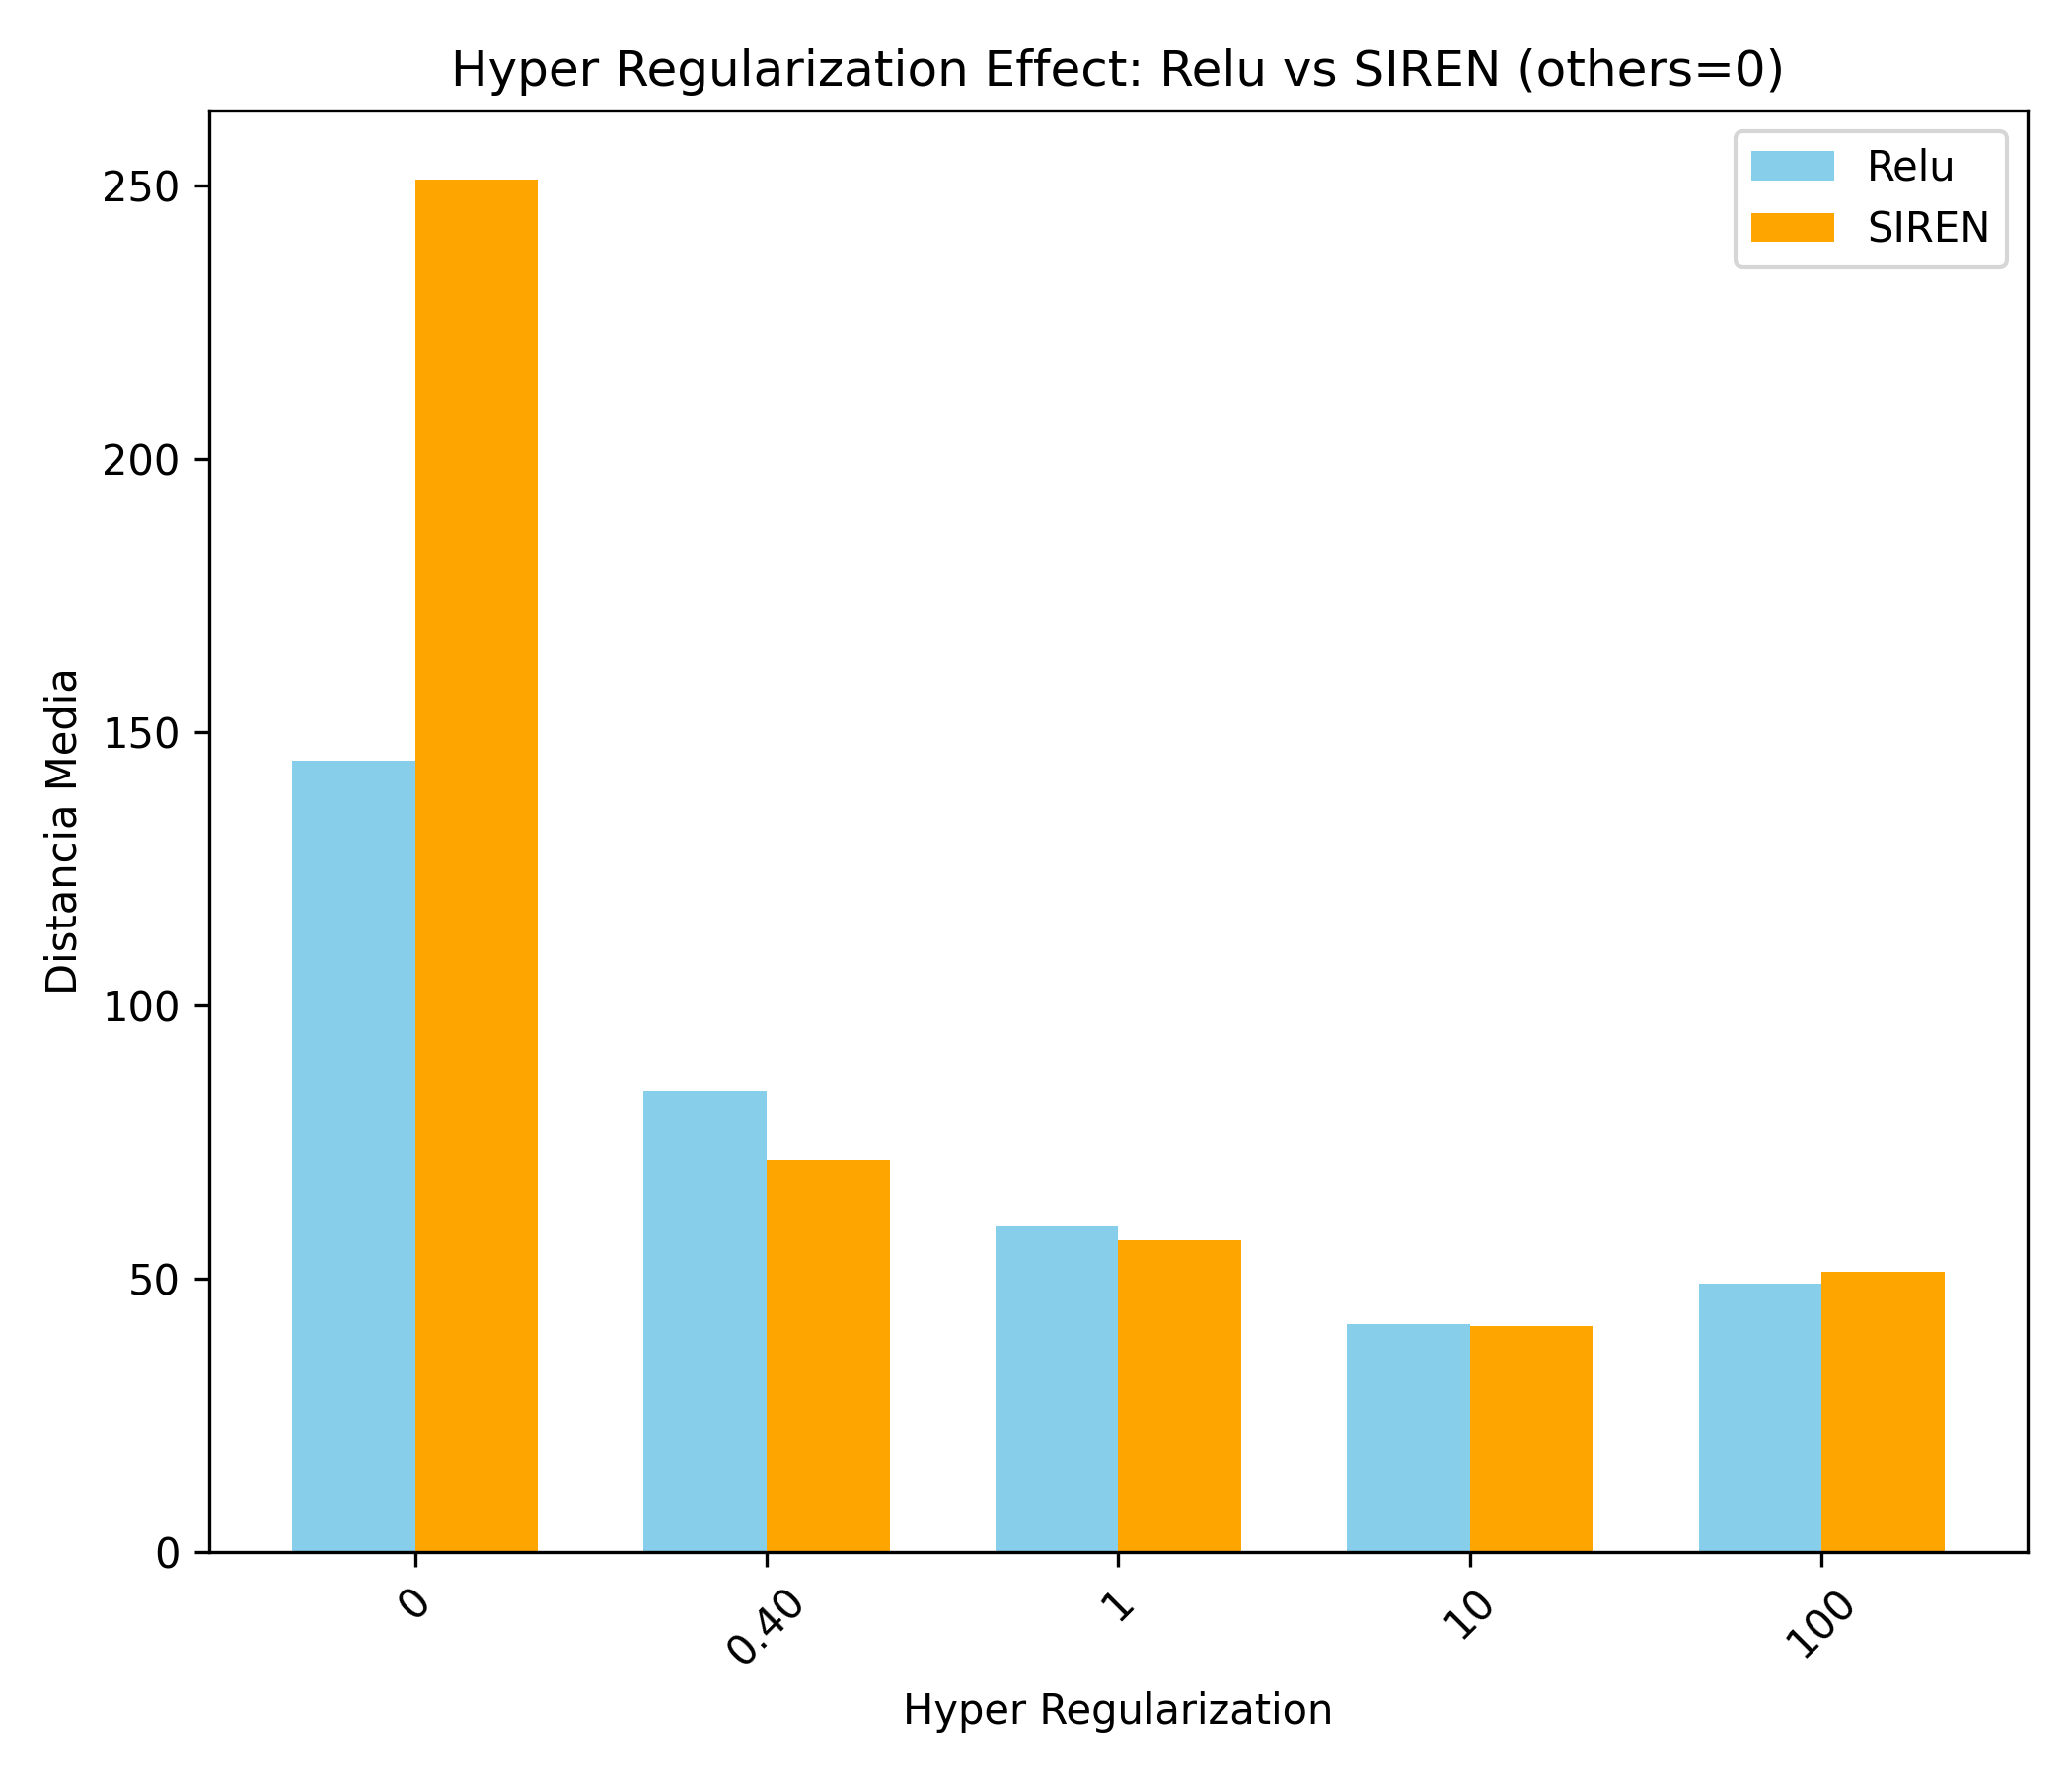
\includegraphics[width=\textwidth]{imaxes/reg_examples/barplot_hyper_reg_comparison_MLP_vs_SIREN_FIRE.png}
        \caption{Comparación de regularización hiperelástica en FIRE}
        \label{fig:barplot_hyper_reg_comparison_MLP_vs_SIREN_FIRE}
    \end{subfigure}\hfill
    \begin{subfigure}[b]{0.48\textwidth}
        \centering
        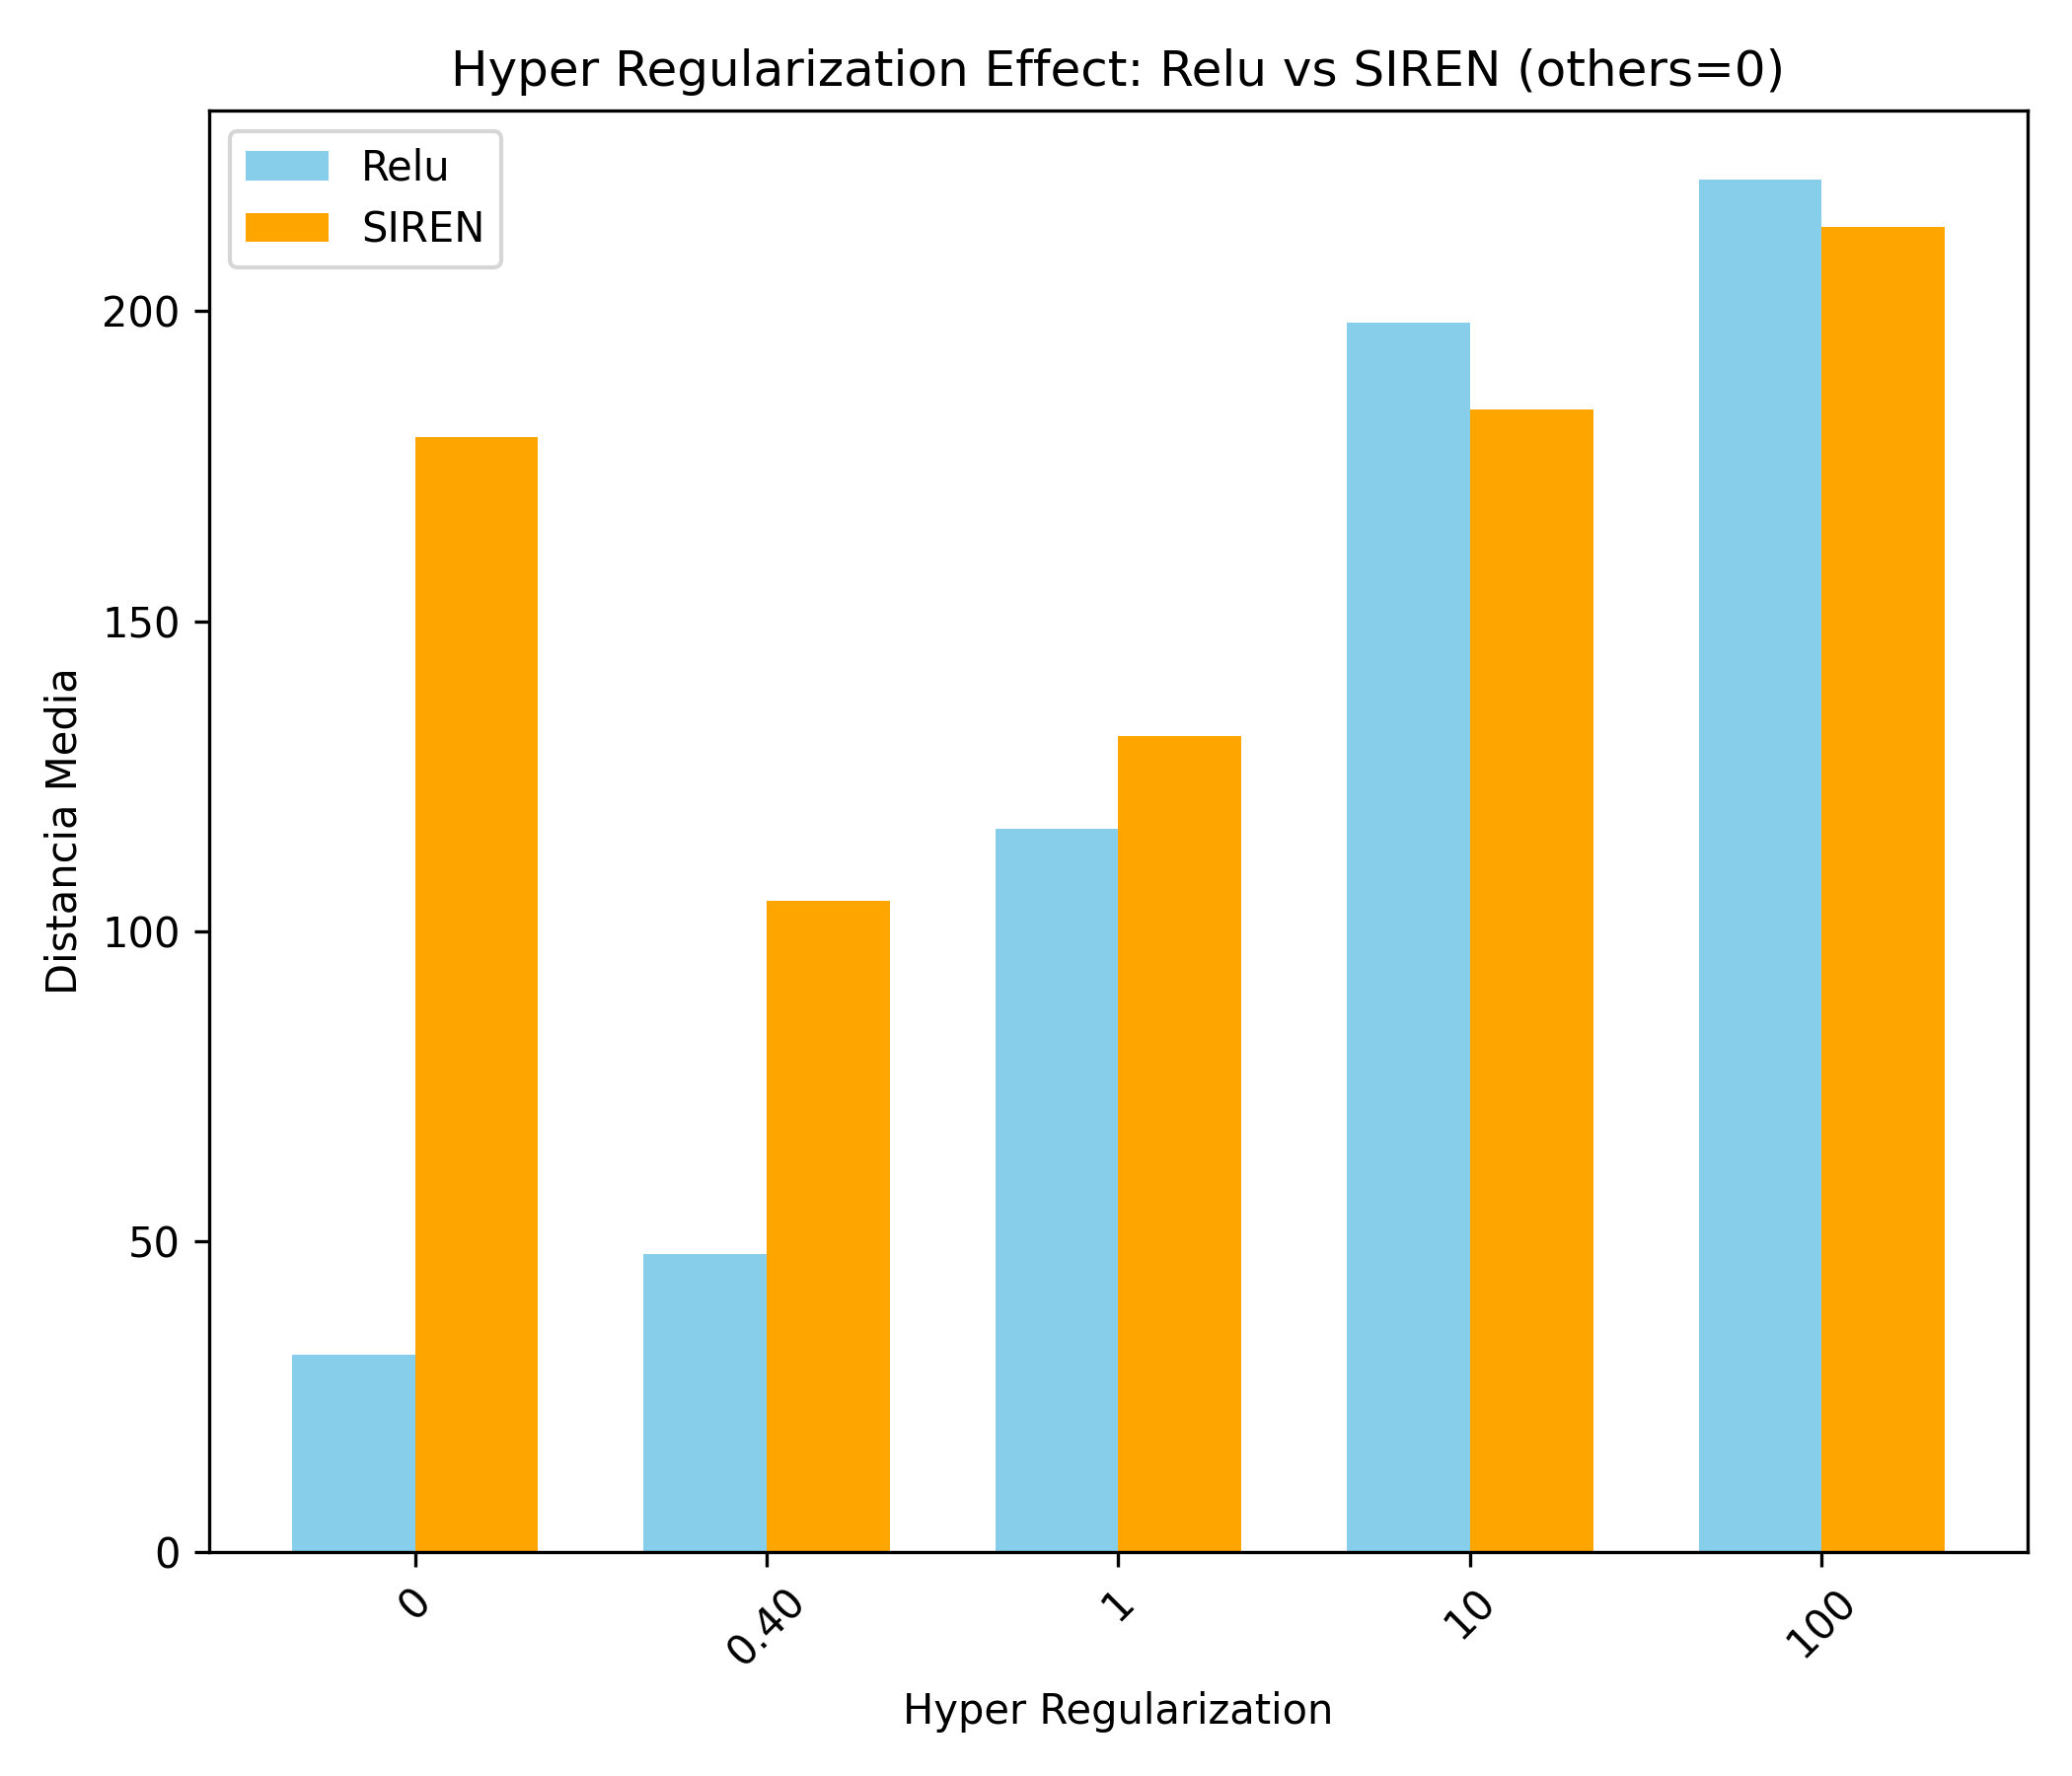
\includegraphics[width=\textwidth]{imaxes/reg_examples/barplot_hyper_reg_comparison_MLP_vs_SIREN_RFMID.png}
        \caption{Comparación de regularización hiperelástica en RFMID}
        \label{fig:barplot_hyper_reg_comparison_MLP_vs_SIREN_RFMID}
    \end{subfigure}
    \caption{Comparación do impacto da regularización hiperelástica sobre os datasets FIRE e RFMID para modelos ReLU e SIREN}
    \label{fig:barplot_hyper_reg_comparison}
\end{figure}

% \FloatBarrier

\subsection{Discusión}
\label{subsec:Discusion-regularization}

Os resultados amosan que a regularización ten un impacto significativo no rendemento da rede. Tanto a ausencia de regularización como a regularización excesiva resultan en rendemento deficiente.
Na figura \ref{fig:regularization_examples} pódense observar exemplos de rexistros con ambos problemas.

\begin{figure}[tbp]
    \centering
    \begin{subfigure}[b]{0.45\textwidth}
        \centering
        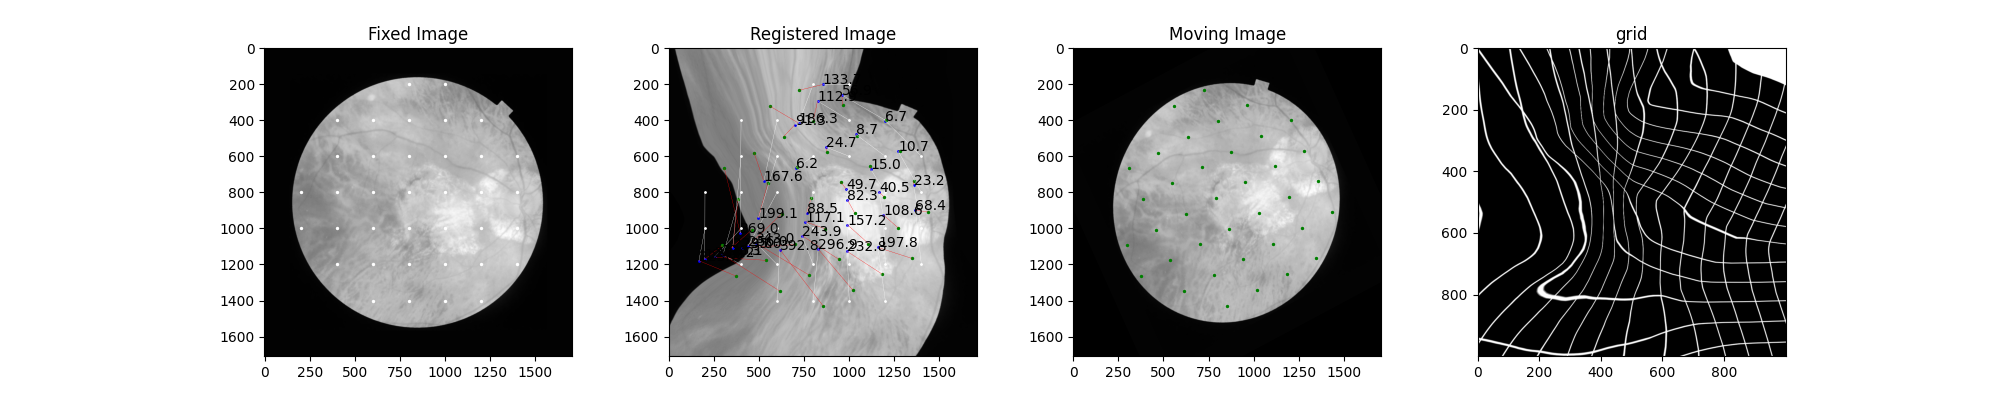
\includegraphics[width=\textwidth]{imaxes/reg_examples/no_reg_example.png}
        \caption{Exemplo de rexistro con cero regularización, o que provoca dobreces}
        \label{fig:no_reg_example}
    \end{subfigure}\hfill
    \begin{subfigure}[b]{0.45\textwidth}
        \centering
        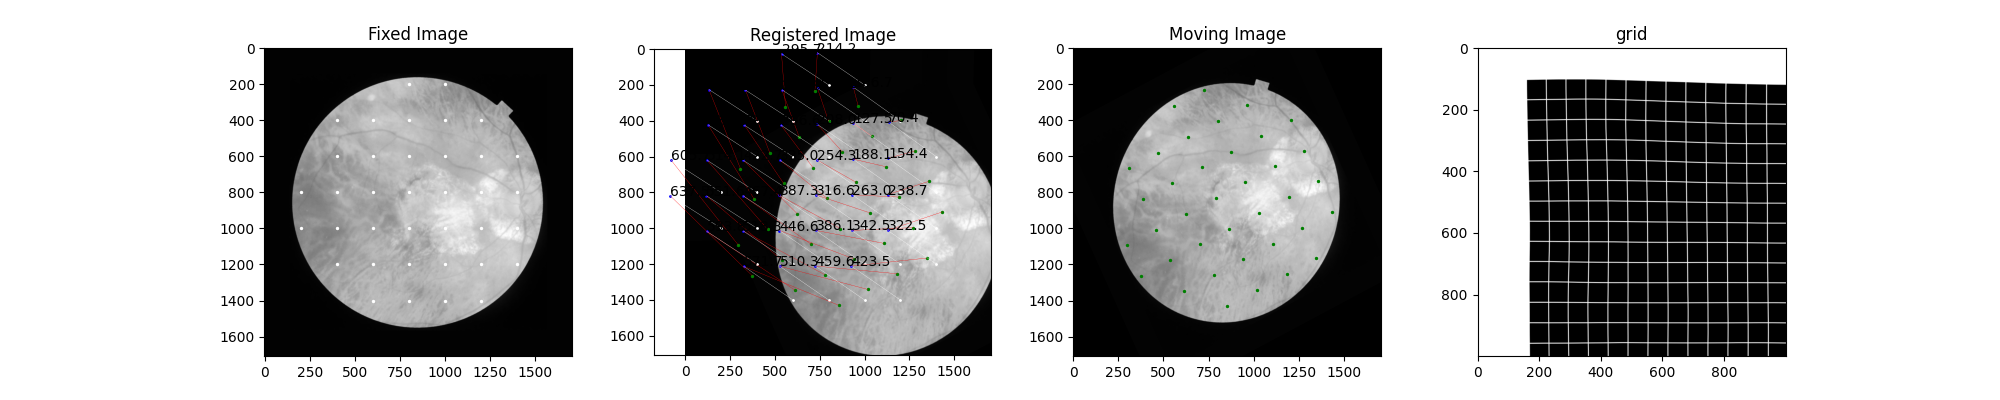
\includegraphics[width=\textwidth]{imaxes/reg_examples/too_much_reg_example.png}
        \caption{Exemplo de rexistro con regularización excesiva, o que evita que a rede aprenda a transformación adecuada}
        \label{fig:too_much_reg_example}
    \end{subfigure}
    \caption{Exemplos de rexistro con ausencia e exceso de regularización}
    \label{fig:regularization_examples}
\end{figure}

Nos resultados obsérvase que Relu segue a dar mellores resultados que SIREN no dataset RFMID, mentres que no dataset FIRE ambos parecen ter un rendemento similar.

A regularización óptima depende do tipo de rexistro que se está a realizar. Os rexistros de transformacións lineais (RFMID) beneficianse de pouca ou ningunha regularización, mentres que os rexistros de transformacións non lineais (FIRE) e con pouca superposición beneficianse de regularizacións mais elevadas.
Isto suxire que a regularización é mais relevante onde a rede ten que aprender transformacións mais complexas, xa que evita que caia en mínimos locais non desexados.

% \FloatBarrier

% \paragraph{Conclusións}
% \label{par:Conclusions-regularization}

% Determínase uns valores razoables para cada un dos termos de regularización, que se utilizarán para os experimentos posteriores.

% \FloatBarrier

% \subsubsection{Learning rate}
% \label{subsubsec:Learning rate}

% \paragraph{Planteamento}
% \label{par:Planteamento-learningrate}

% Para determinar cal é o learning rate óptimo, realizáronse experimentos comparando o rendemento de cada un sobre unha mostra de imaxes dos datases de FIRE e RFMID cas diferentes funcións de activación.
% Tamñen se experimentou con diferentes batch sizes para determinar a relación entre ambos.

% \paragraph{Resultados}
% \label{par:Resultados-learningrate}

% Están solo sobre category S de FIRE

% \ref{fig:grid_search_lr}, \ref{fig:e_heatmap_MLP_RFMID}

% \begin{figure}[tbp]
%     \centering
%     \begin{subfigure}[b]{0.45\textwidth}
%         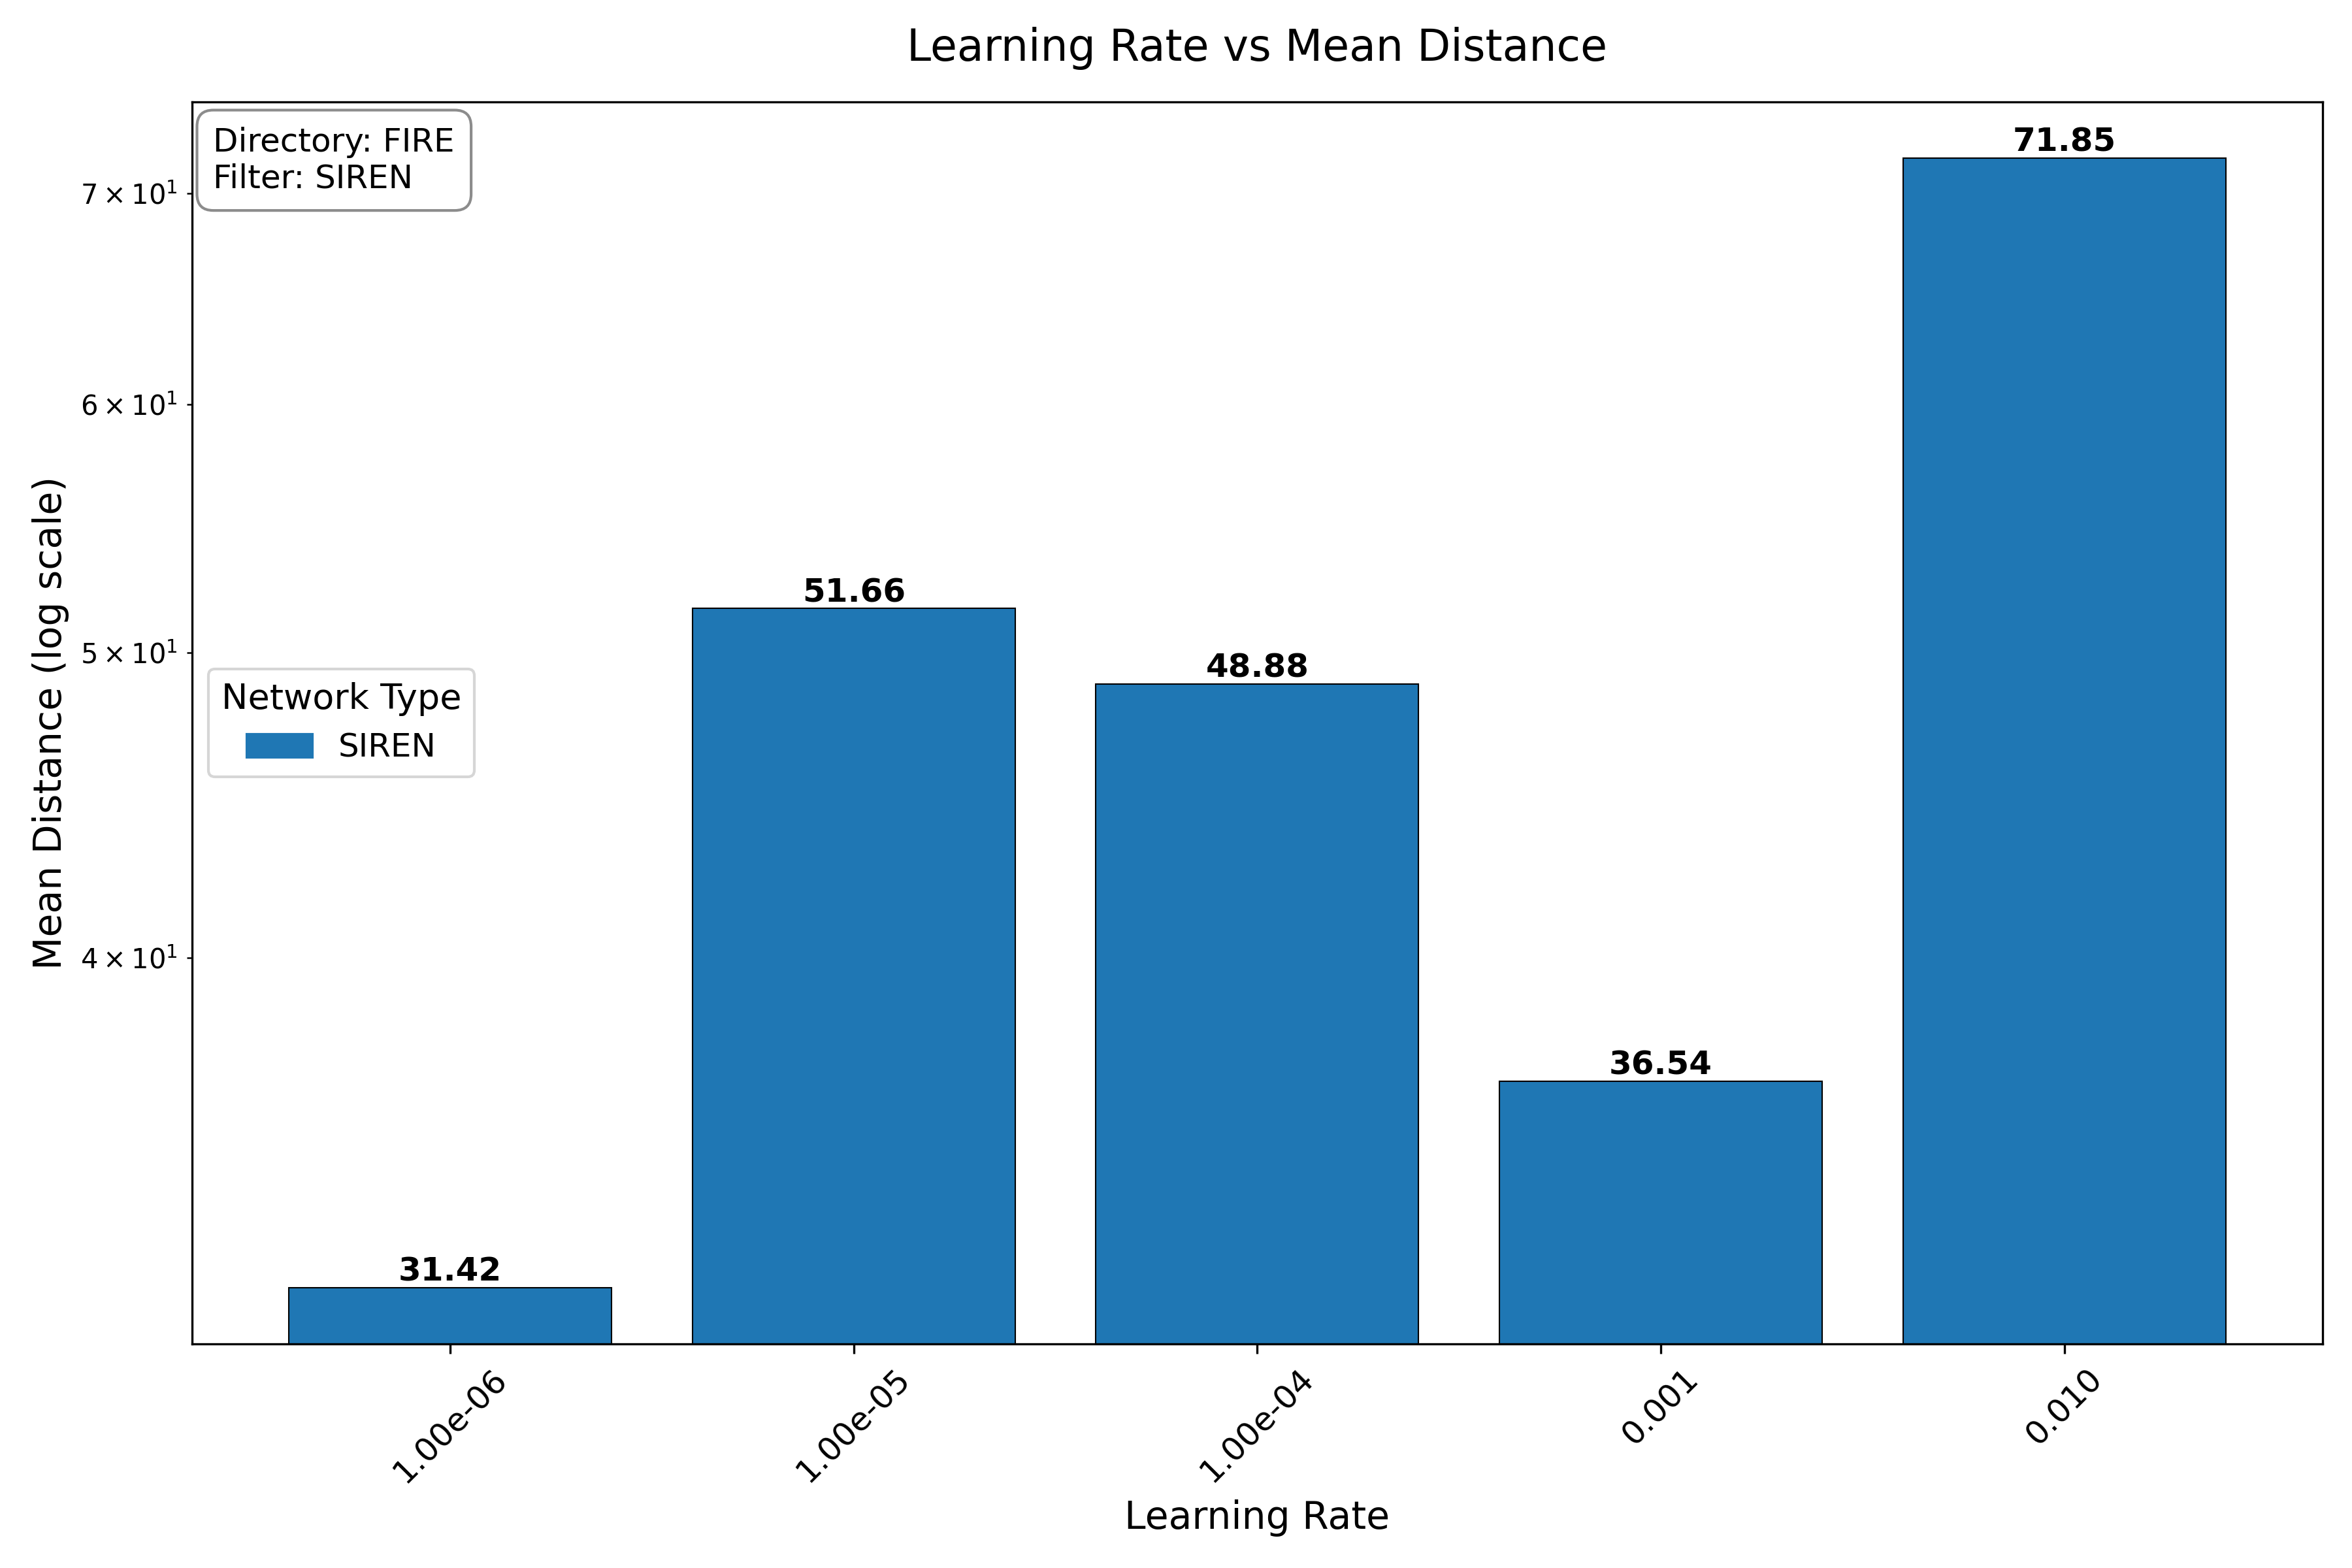
\includegraphics[width=\textwidth]{imaxes/grid_search_lr_FIRE_SIREN.png}
%         \caption{FIRE - SIREN}
%         \label{fig:grid_search_lr_FIRE_SIREN}
%     \end{subfigure}\hfill
%     \begin{subfigure}[b]{0.45\textwidth}
%         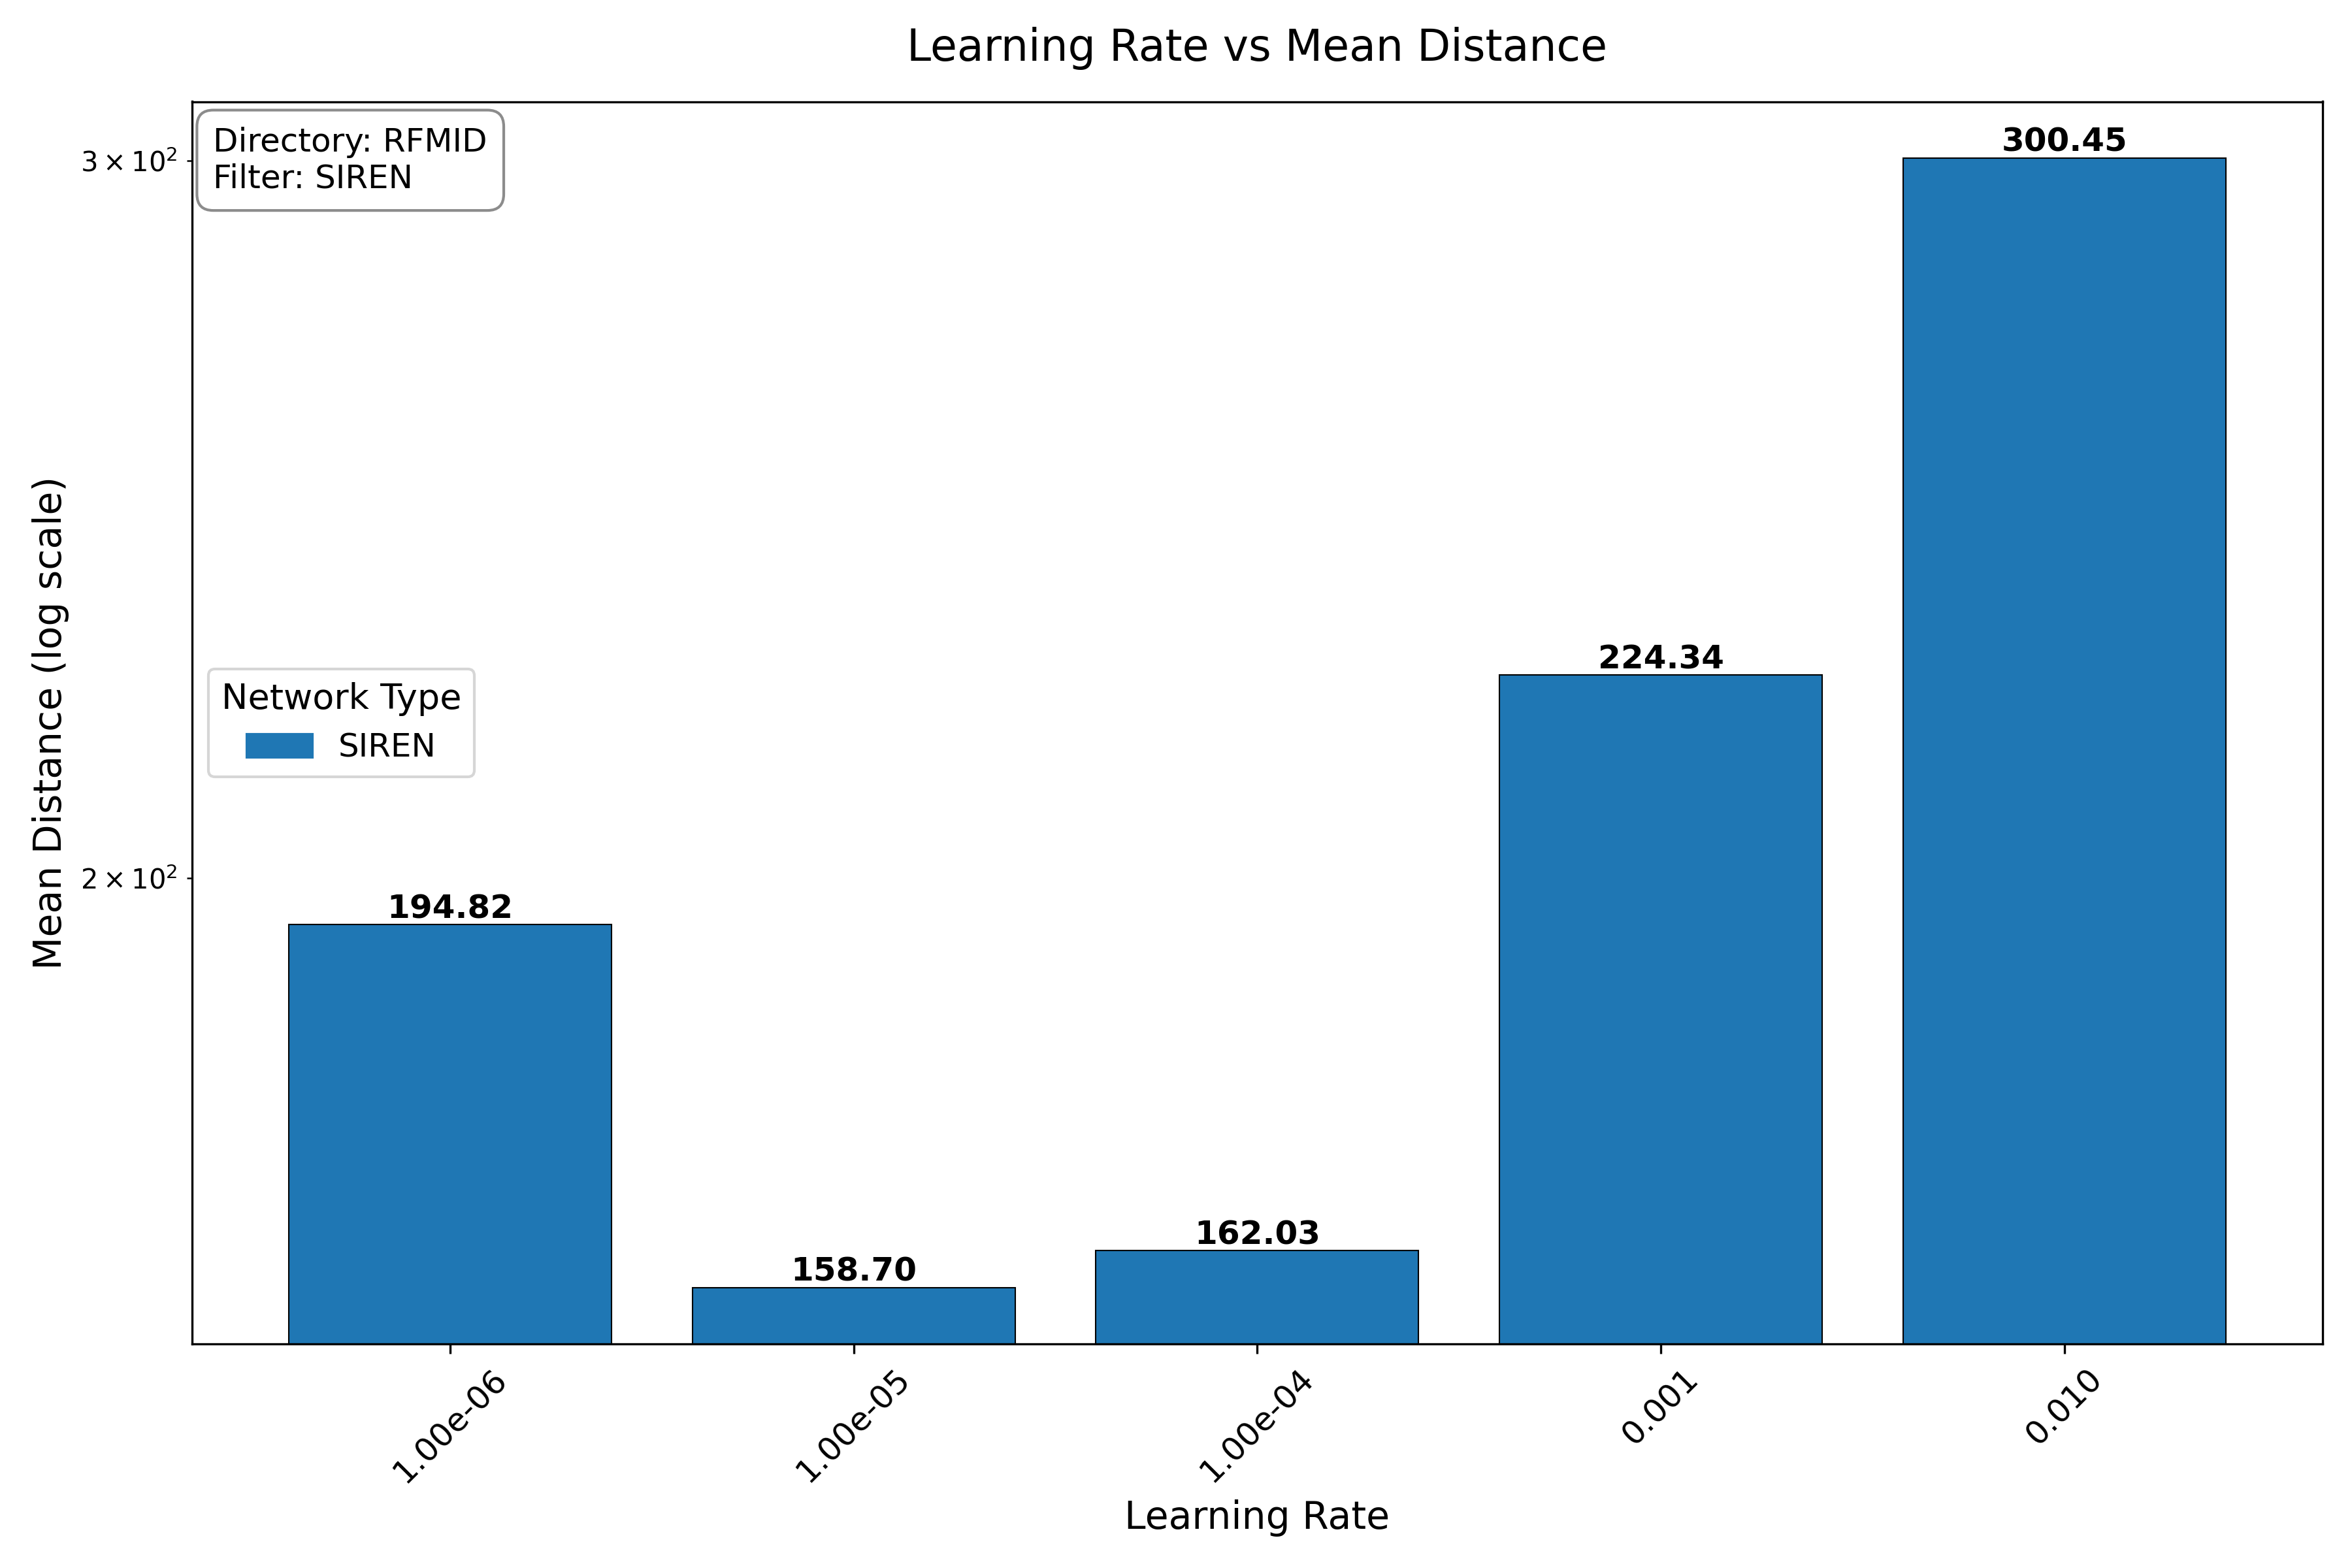
\includegraphics[width=\textwidth]{imaxes/grid_search_lr_RFMID_SIREN.png}
%         \caption{RFMID - SIREN}
%         \label{fig:grid_search_lr_RFMID_SIREN}
%     \end{subfigure}
%     \vskip\baselineskip
%     \begin{subfigure}[b]{0.45\textwidth}
%         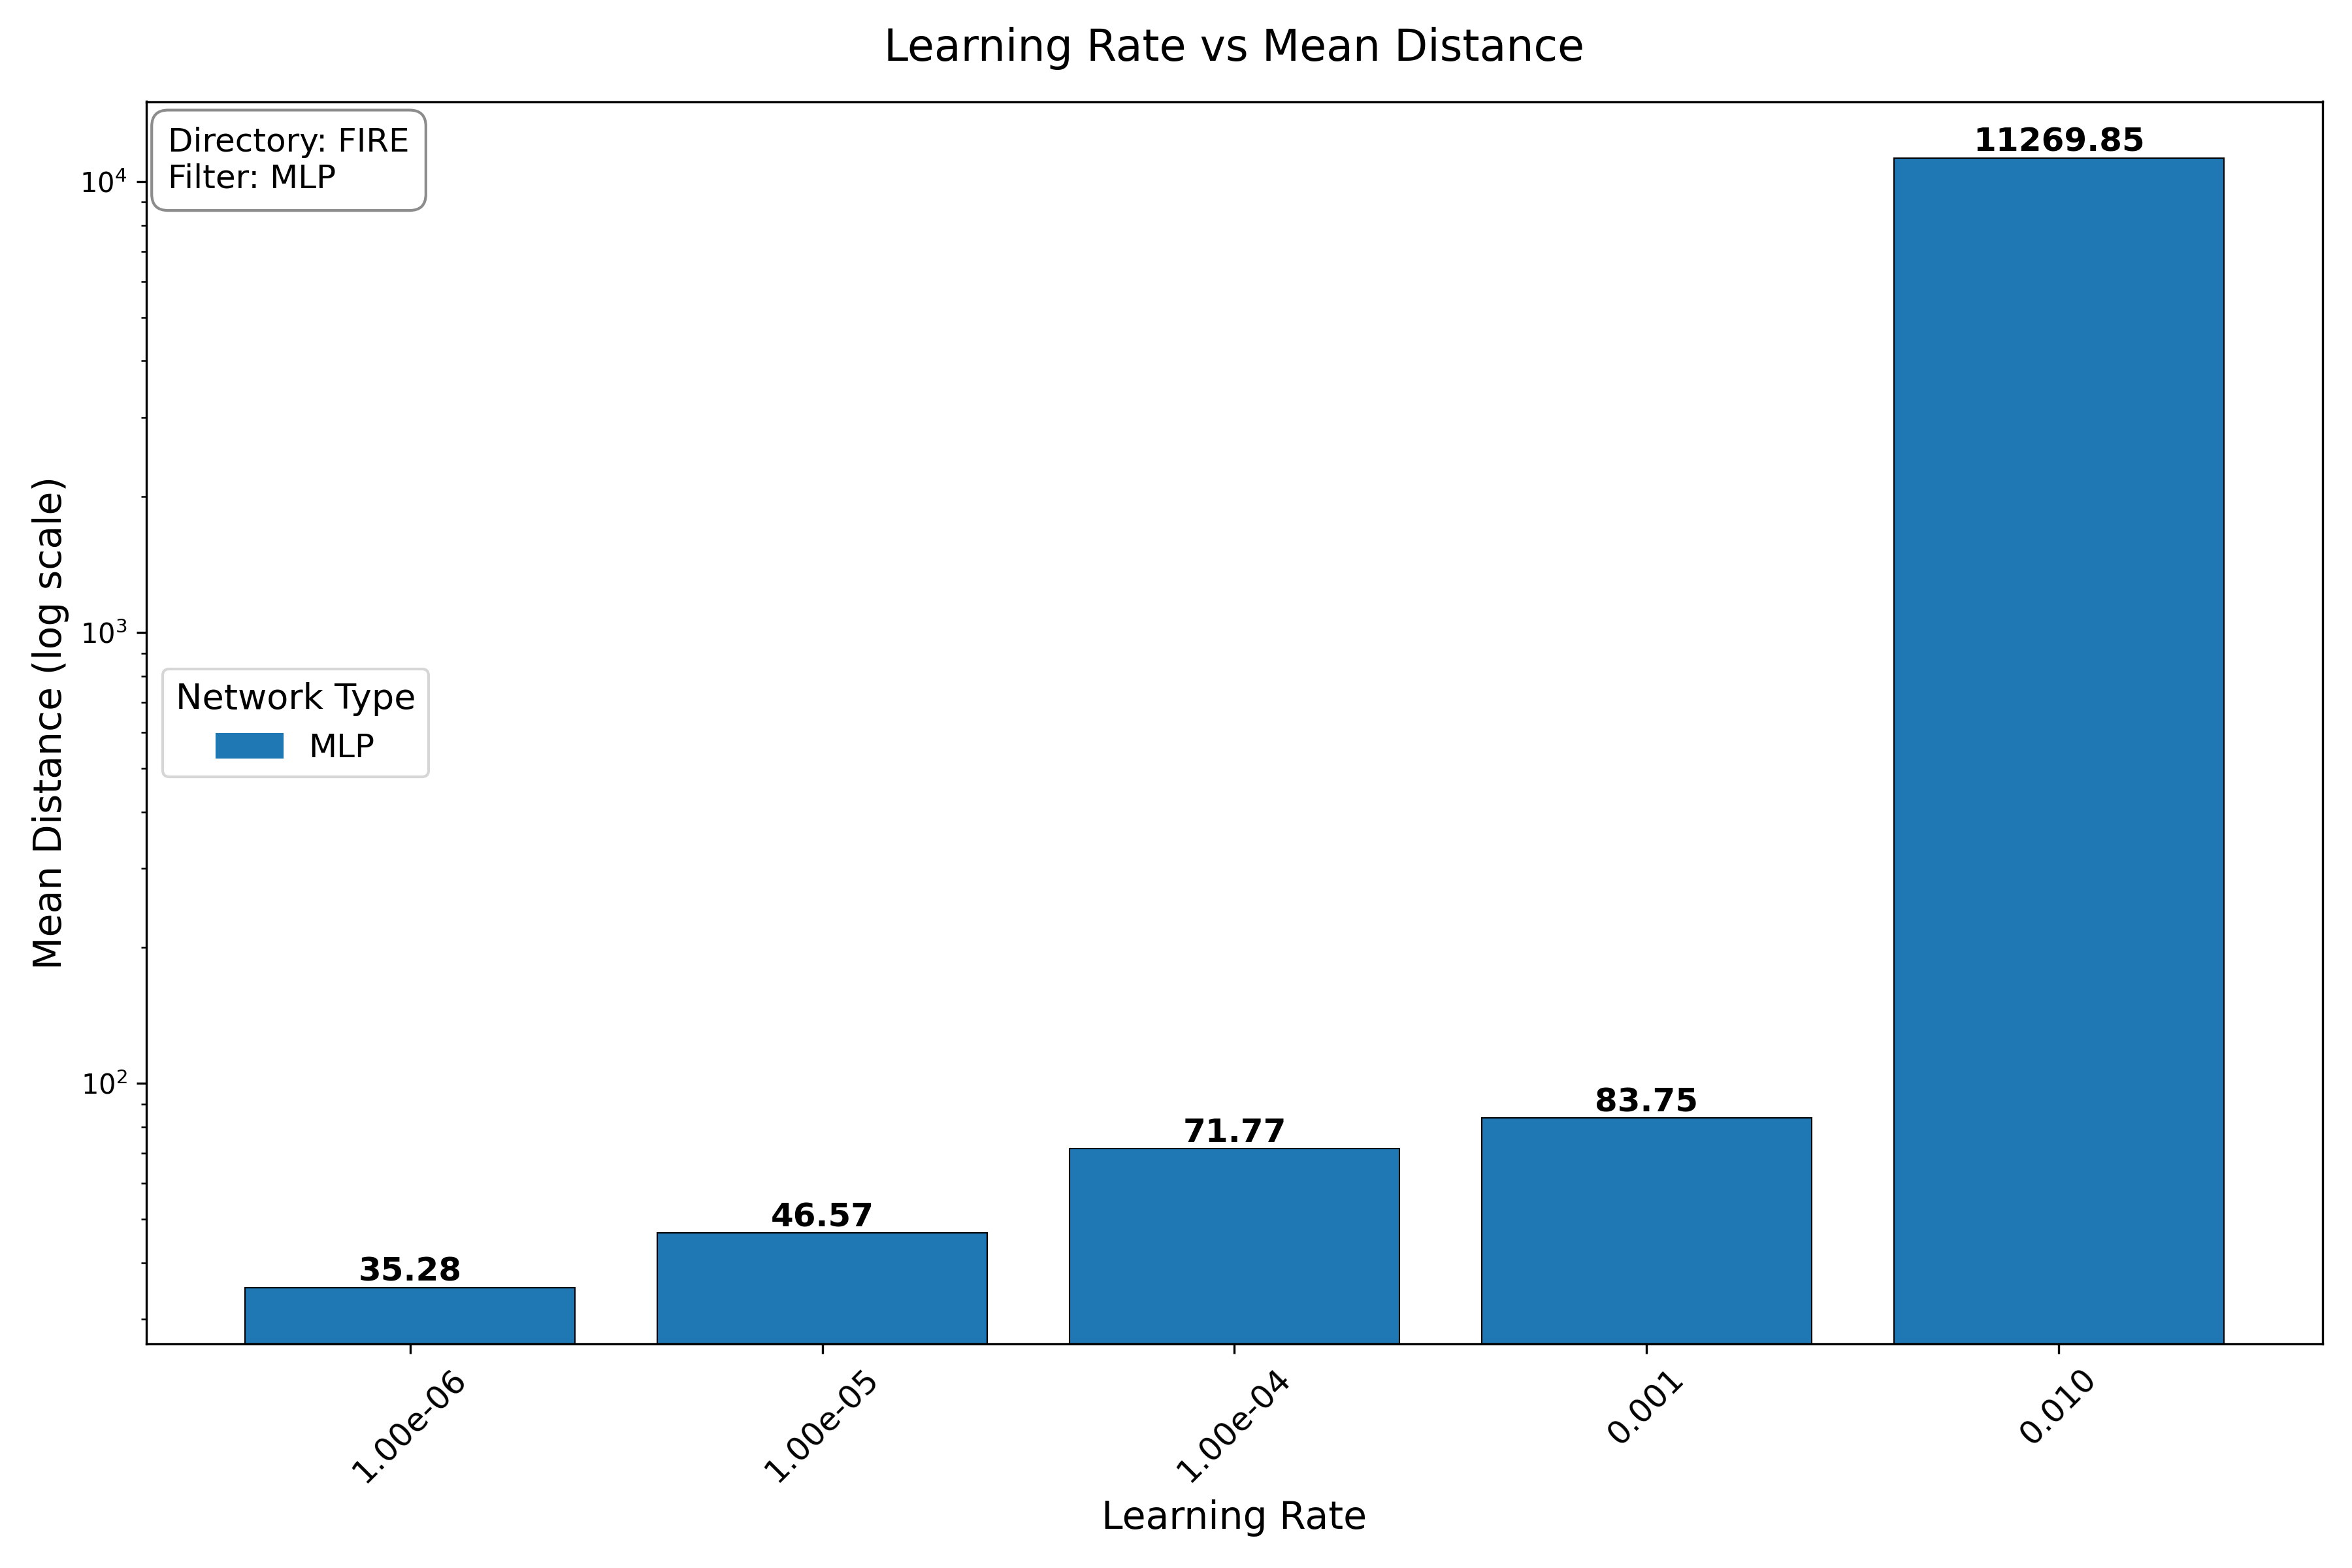
\includegraphics[width=\textwidth]{imaxes/grid_search_lr_FIRE_MLP.png}
%         \caption{FIRE - Relu}
%         \label{fig:grid_search_lr_FIRE_MLP}
%     \end{subfigure}\hfill
%     \begin{subfigure}[b]{0.45\textwidth}
%         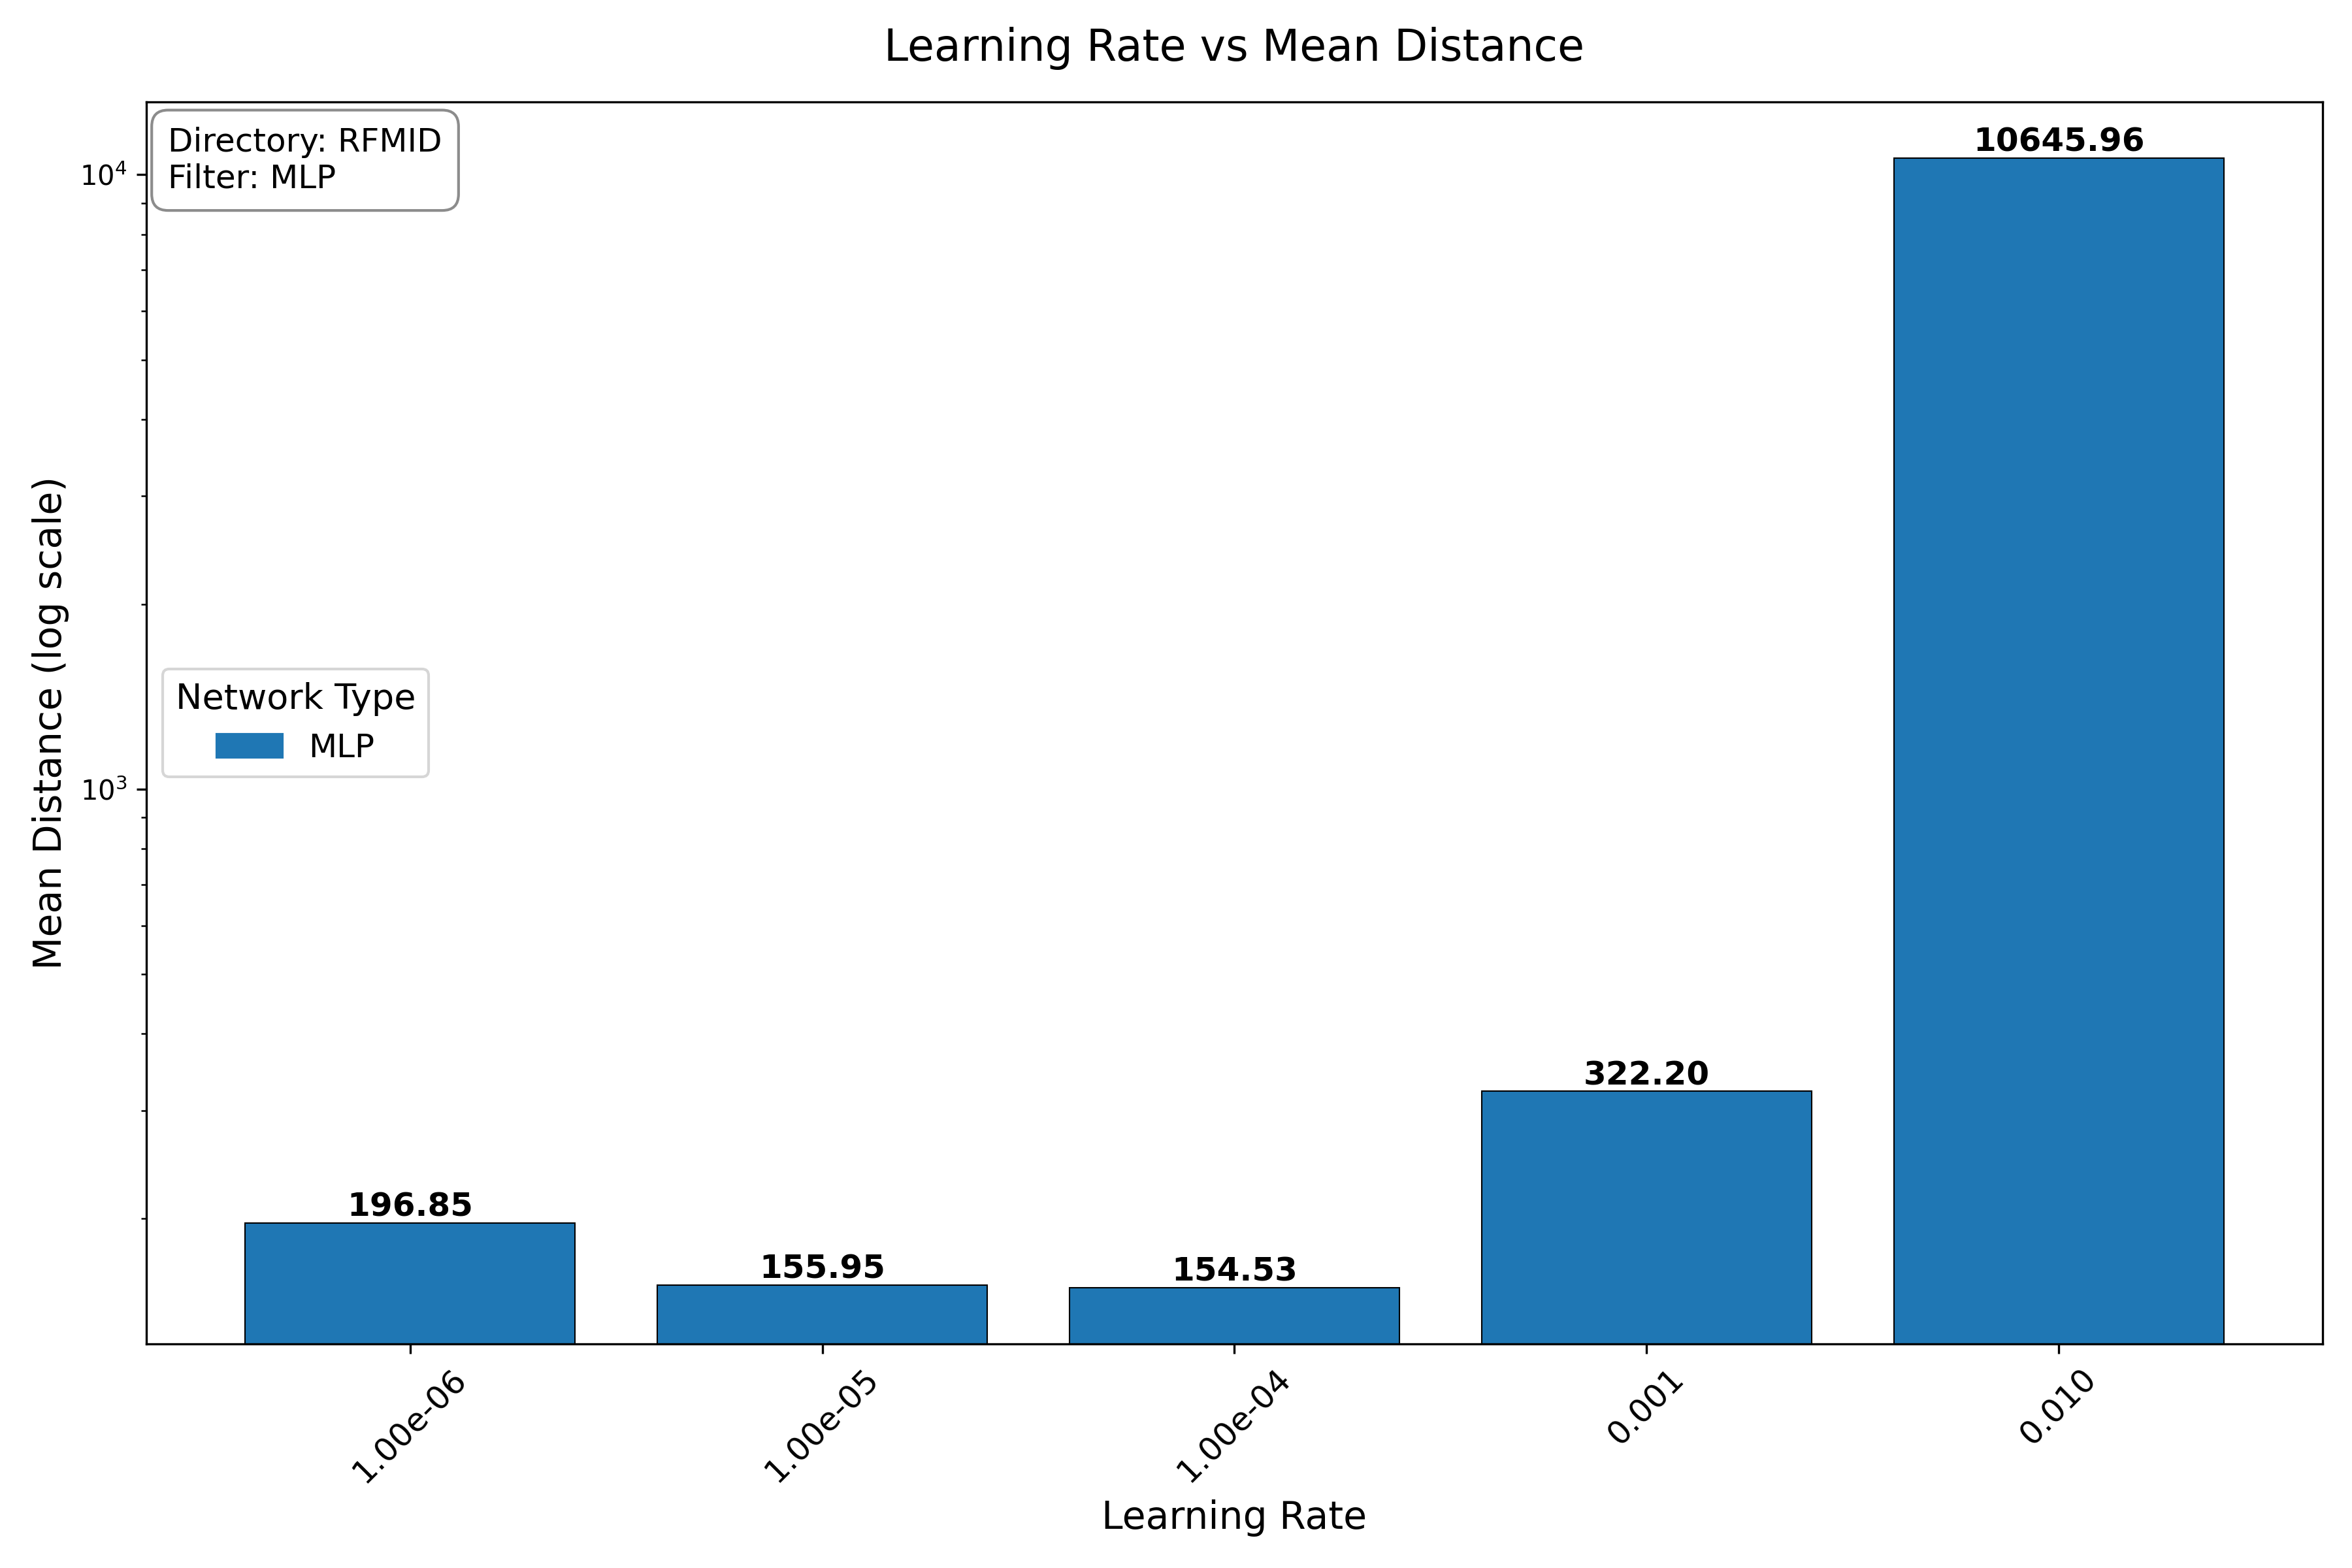
\includegraphics[width=\textwidth]{imaxes/grid_search_lr_RFMID_MLP.png}
%         \caption{RFMID - Relu}
%         \label{fig:grid_search_lr_RFMID_MLP}
%     \end{subfigure}
%     \caption{Resultados lr cos datasets FIRE e RFMID cas funcións de activación SIREN e Relu.}
%     \label{fig:grid_search_lr}
% \end{figure}

% \begin{figure}[tbp]
%     \centering
%     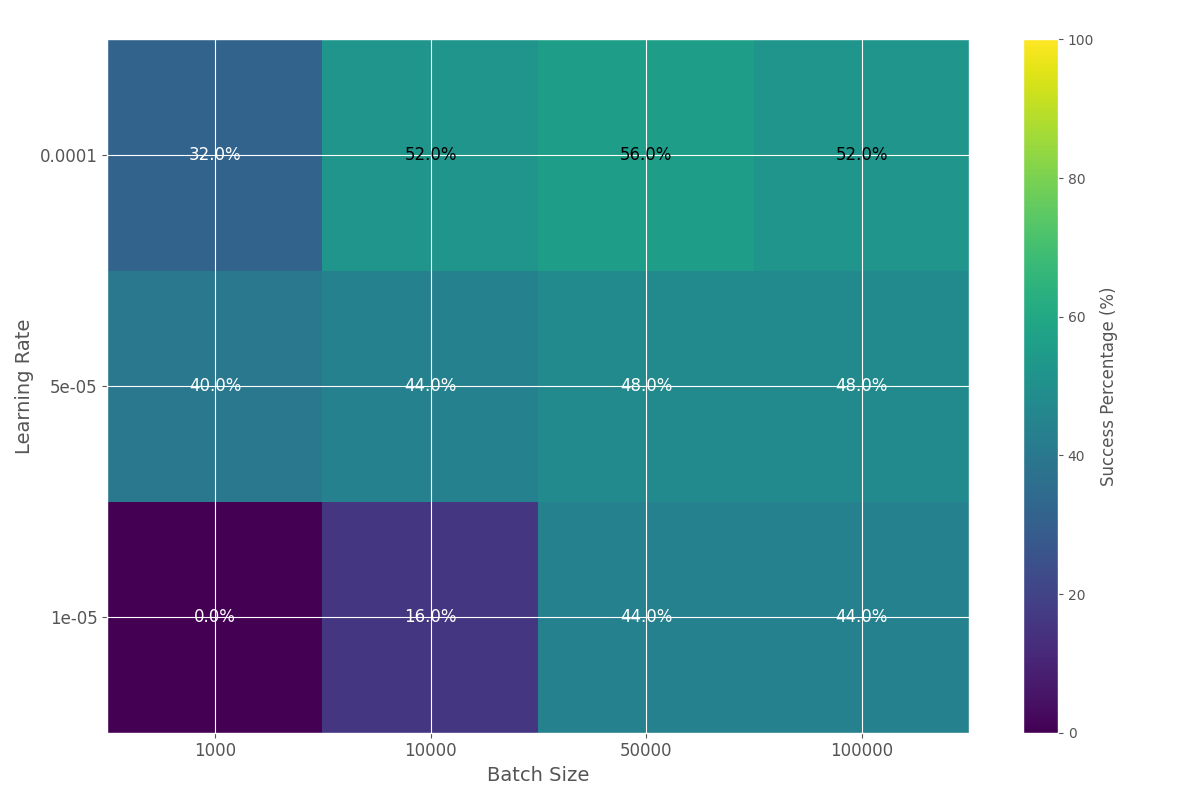
\includegraphics[width=0.8\textwidth]{imaxes/e_heatmap_MLP_RFMID.png}
%     \caption{Mapa de calor cos resultados de diferentes combinacións de tamaño de lote e learning rate con unha mostra de imaxes de RMIFD ca función de activación ReLU}
%     \label{fig:e_heatmap_MLP_RFMID}
% \end{figure}

% \FloatBarrier

% \paragraph{Discusión}
% \label{par:Discusion-learningrate}

% Valores de learning rate moi altos (0.001 and 0.005) son contraproducentes, xa que a rede diverxe rapidamente.

% A dependencia entre o learning rate e o tamaño de lote confirmase. Xeralmente un learning rate baixo (1.0e-05, 1.0e-06) parece requerir de batch sizes maiores e viceversa, o cal é consistente co que se esperaba.

% Tamén observase que batch sizes maiores tenden a dar mellores resultados.

% \paragraph{Conclusións}
% \label{par:Conclusions-learningrate}

\subsection{Conclusións}
\label{subsec:Conclusions-regularization}

En base aos resultados, conclúese que a regularización é un compoñente indispensable para o rexistro de retinas con redes implícitas. O seu valor óptimo non é universal, senón que depende directamente da complexidade da transformación a aprender. Para deformacións sinxelas e lineais como as de RFMiD, unha regularización mínima é suficiente, pero para os desafíos presentes en FIRE, cunha maior non linearidade, un termo de regularización robusto é crucial para guiar a rede cara a solucións fisicamente plausibles e evitar o sobreaxuste. Confírmase tamén que os modelos SIREN, pola súa maior capacidade para representar detalles de alta frecuencia, son máis sensibles á regularización e requiren valores xeralmente máis altos que os modelos ReLU para previr artefactos. A elección do coeficiente de regularización debe considerarse unha decisión fundamental, adaptada tanto á natureza do problema de rexistro como á arquitectura da rede empregada.

\section{Tamaño de lote}
\label{sec:Tamaño de lote}

\subsection{Planteamento}
\label{subsec:Planteamento-batchsize}

Ao longo dos experimentos realizados, o análisis cualitativo revelou que o tamaño de lote é un dos parámetros que máis impacto ten no rendemento da rede.

De agora en adiante dividimos o conxunto de datos de RFMID en varios subconxuntos según a dificultade da transformación, como detallado na seccion \ref{subsec:Avaliación Cuantitativa}.

Desta forma podemos comparar o rendemento da rede en diferentes subconxuntos de imaxes, e determinar se o rendemento da rede é consistente entre eles.

Nos experimentos co dataset FIRE, decidiuse limitarse á categoría S, xa que é a que maior número de exemplos tén e ten un maior grao de superposición entre as imaxes, o que facilita a tarefa de rexistro.
Ademais, xa que a rede si que é capaz de rexistrar correctamente as imaxes dos subconxuntos mais sinxelos, utilizaremos a métrica de FIRE para medir o porcentaxe de imaxes rexistradas correctamente.

\subsection{Resultados}
\label{subsec:Resultados-batchsize}

Nas figuras \ref{fig:batch_size_comparison_relu_rfmid} e \ref{fig:batch_size_comparison_siren_rfmid} pódense observar os resultados da experimentación co dataset RFMID a distintas dificultades e con distintos tamaños de batch.

\begin{figure}[tbp]
    \centering
    \begin{subfigure}[b]{0.5\textwidth}
        \centering
        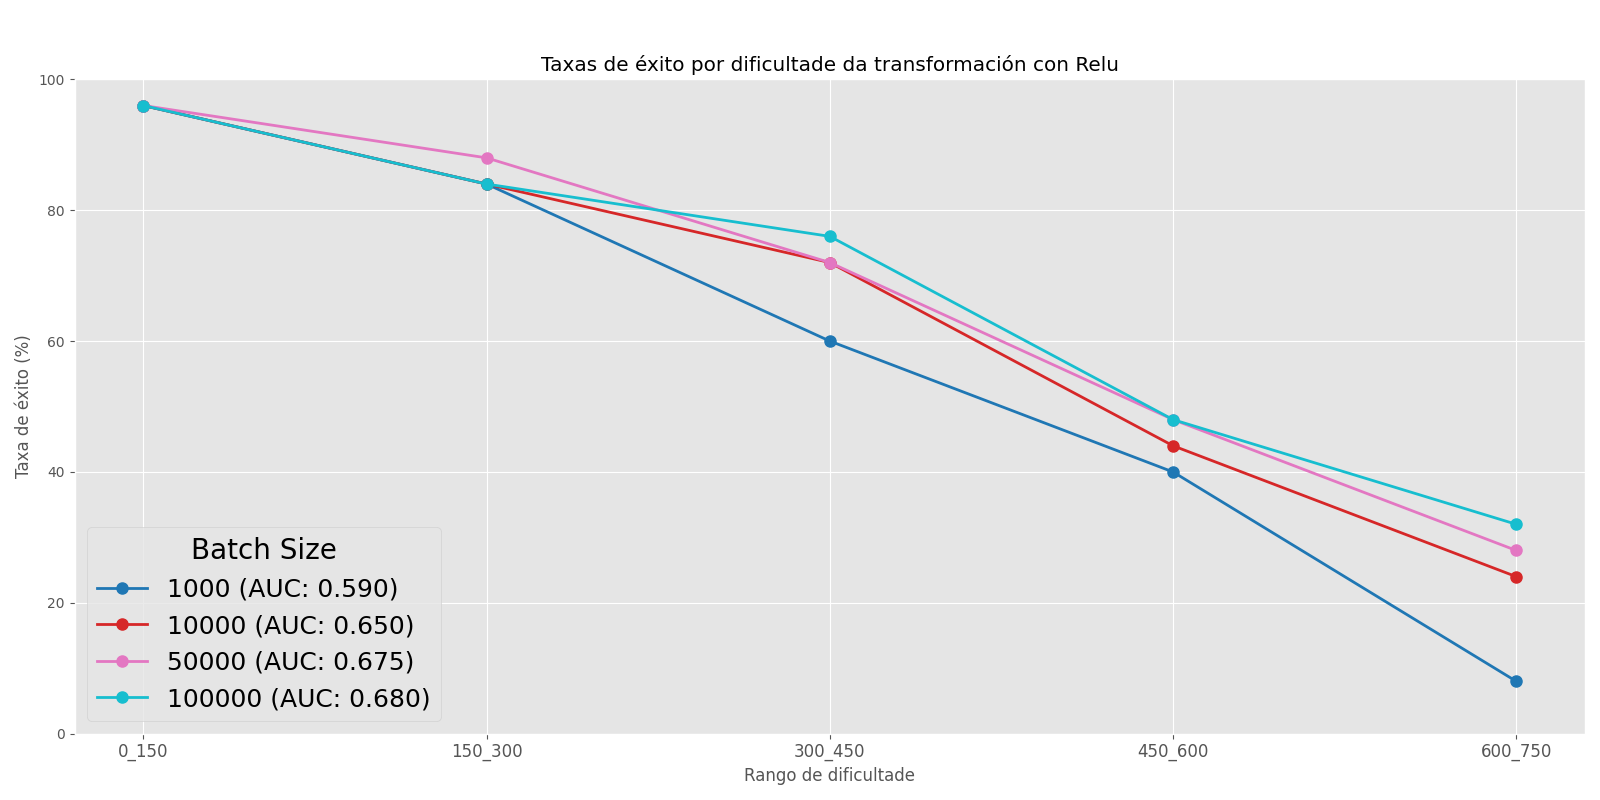
\includegraphics[width=\textwidth]{imaxes/batchsize/experiment_plot_RFMID_bs_relu.png}
        \caption{Función de activación ReLU}
        \label{fig:batch_size_comparison_relu_rfmid}
    \end{subfigure}\hfill
    \begin{subfigure}[b]{0.5\textwidth}
        \centering
        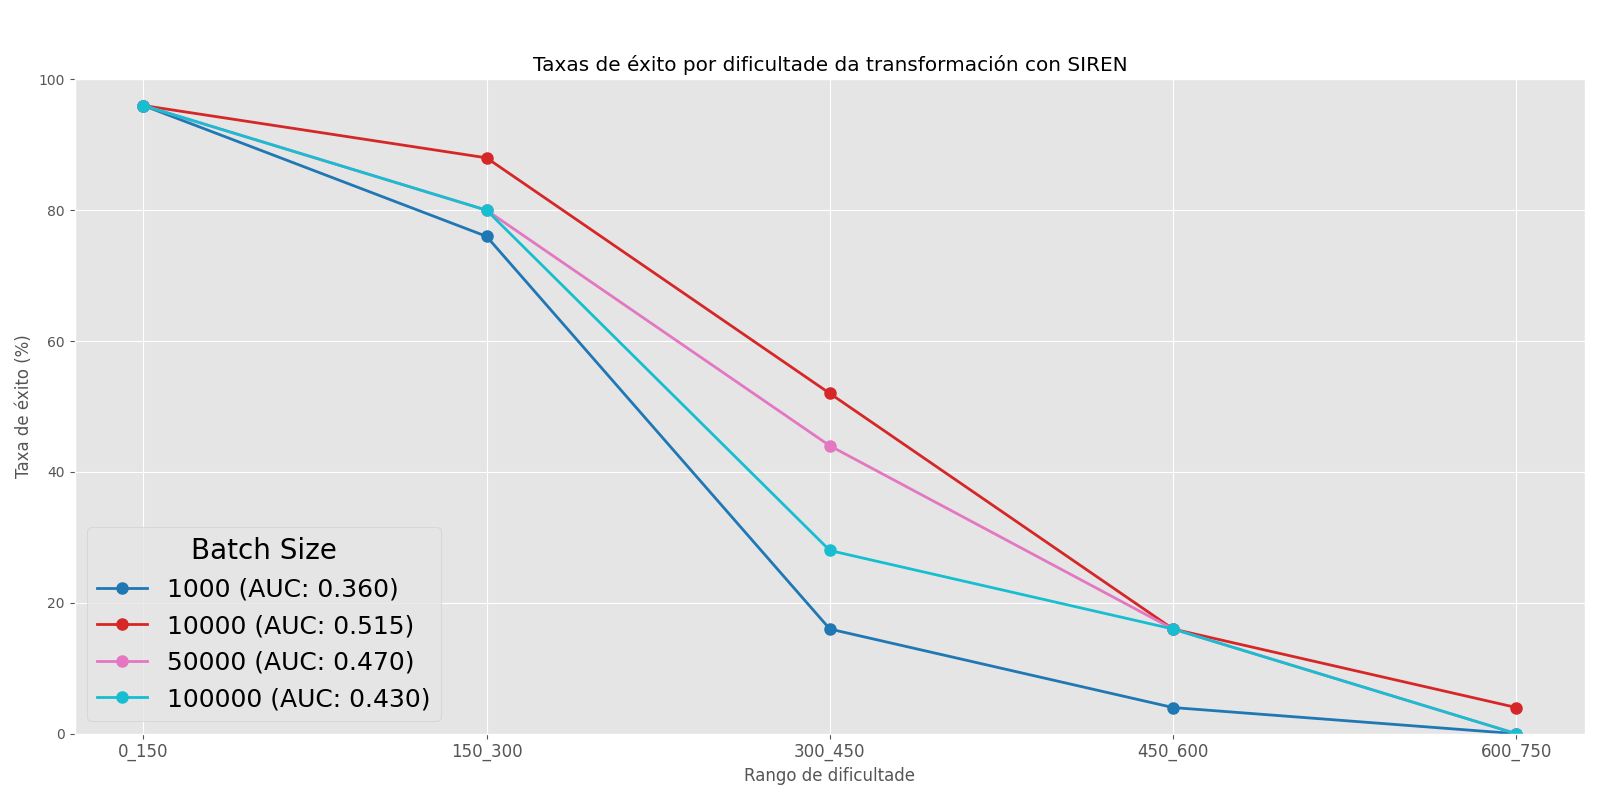
\includegraphics[width=\textwidth]{imaxes/batchsize/experiment_plot_RFMID_bs_siren.png}
        \caption{Función de activación SIREN}
        \label{fig:batch_size_comparison_siren_rfmid}
    \end{subfigure}
    \caption{Comparación do rendemento da rede con diferentes batch sizes sobre imaxes do dataset RFMID, mostrando a porcentaxe de rexistros exitoso para cada limiar de error.}
    \label{fig:batch_size_comparisons_rfmid}
\end{figure}

Con esta nova división do dataset, tamén se realizou a avaliación polo método de avaliación de FIRE, que se pode ver na figuras \ref{fig:FIRERFMID_relu} e \ref{fig:FIRERFMID_SIREN}.

\begin{figure}[tbp]
    \centering
    \begin{subfigure}[b]{0.5\textwidth}
        \centering
        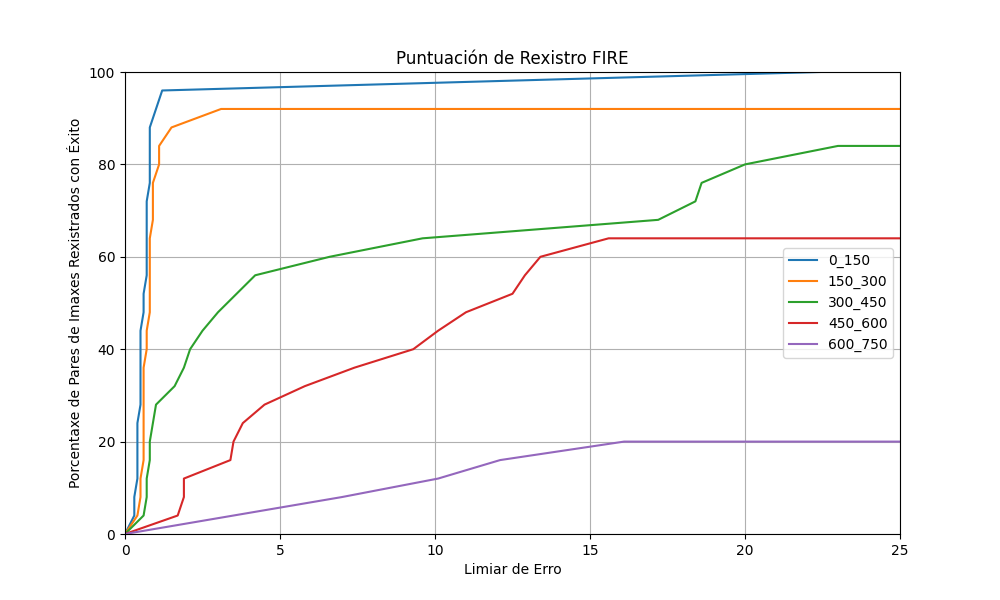
\includegraphics[width=\textwidth]{imaxes/FIRE_scores/fire_registration_scores_RFMID_MLP.png}
        \caption{Métrica FIRE ca función de activación ReLU}
        \label{fig:FIRERFMID_relu}
    \end{subfigure}\hfill
    \begin{subfigure}[b]{0.5\textwidth}
        \centering
        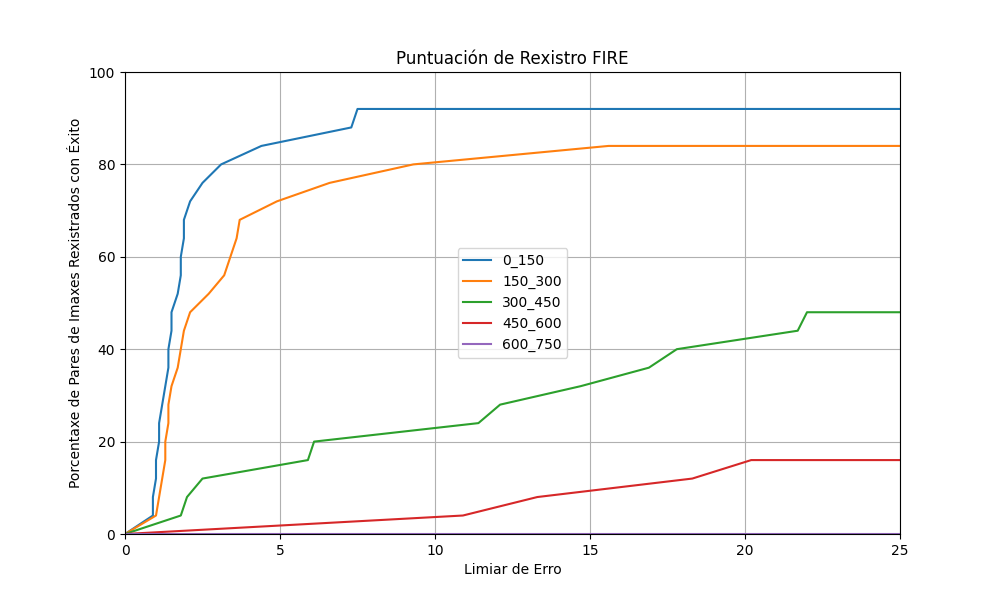
\includegraphics[width=\textwidth]{imaxes/FIRE_scores/fire_registration_scores_RMIFD_SIREN.png}
        \caption{Métrica FIRE ca función de activación SIREN}
        \label{fig:FIRERFMID_SIREN}
    \end{subfigure}
    \caption{Comparación do rendemento da rede con diferentes batch sizes sobre imaxes do dataset FIRE}
    \label{fig:FIRERFMID_scores}
\end{figure}


Nas figuras \ref{fig:batch_size_comparison_relu} e \ref{fig:batch_size_comparison_siren} mostranse os resultados da experimentación co dataset FIRE.

% \ref{fig:batch_size_comparison_relu_1e-5}, \ref{fig:batch_size_comparison_relu_5e-5}, \ref{fig:batch_size_comparison_relu_1e-4}
\begin{figure}[tbp]
    \centering
    \begin{subfigure}[b]{0.5\textwidth}
        \centering
        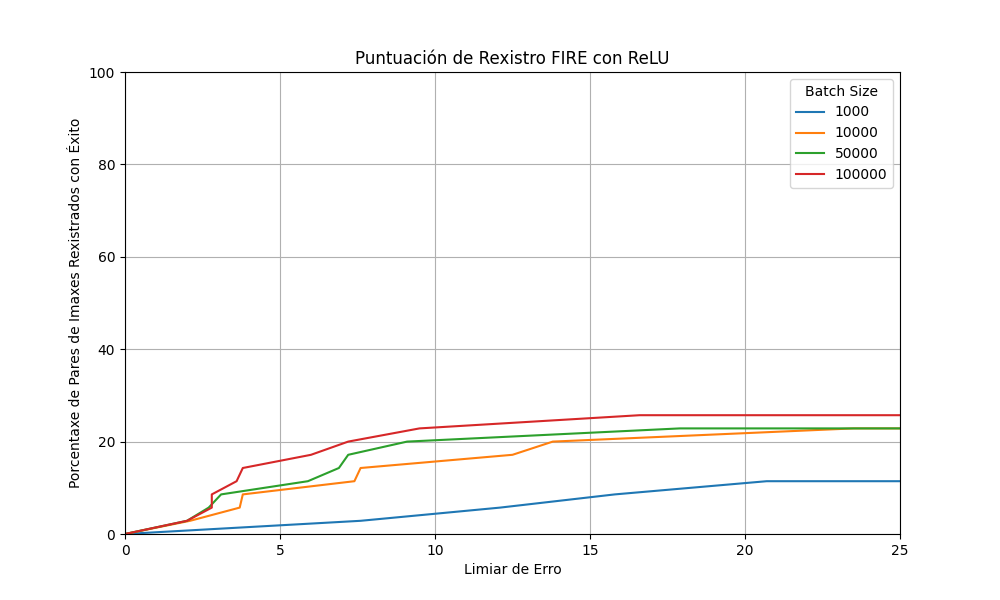
\includegraphics[width=\textwidth]{imaxes/batchsize/fire_registration_scores_bs_relu_S.png}
        \caption{Función de activación ReLU}
        \label{fig:batch_size_comparison_relu}
    \end{subfigure}\hfill
    \begin{subfigure}[b]{0.5\textwidth}
        \centering
        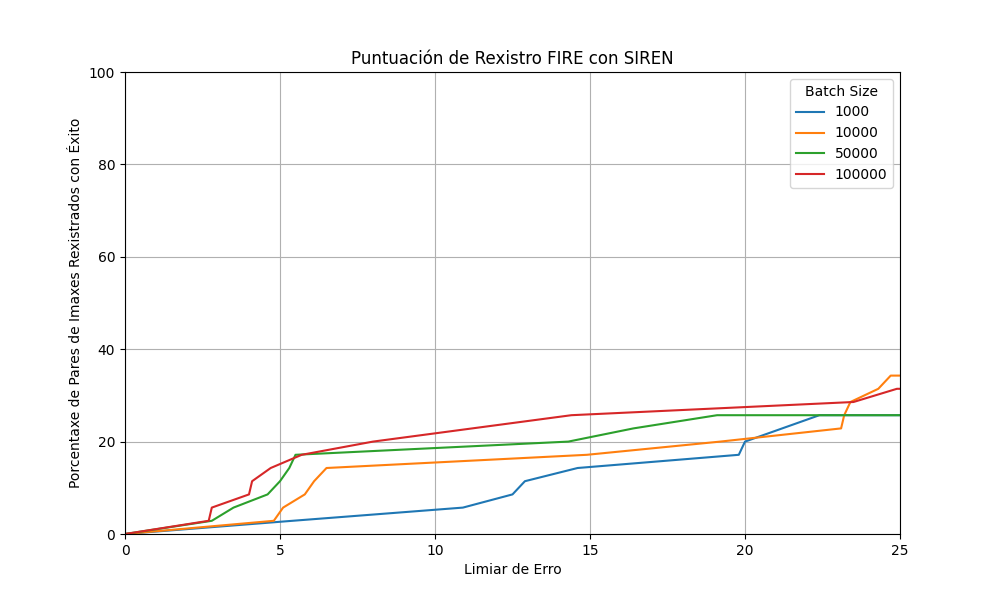
\includegraphics[width=\textwidth]{imaxes/batchsize/fire_registration_scores_bs_siren_S.png}
        \caption{Función de activación SIREN}
        \label{fig:batch_size_comparison_siren}
    \end{subfigure}
    \caption{Comparación do rendemento da rede con diferentes batch sizes sobre imaxes da categoría S do dataset FIRE}
    \label{fig:batch_size_comparisons_fire}
\end{figure}



% \begin{figure}[tbp] 
%     \centering
%     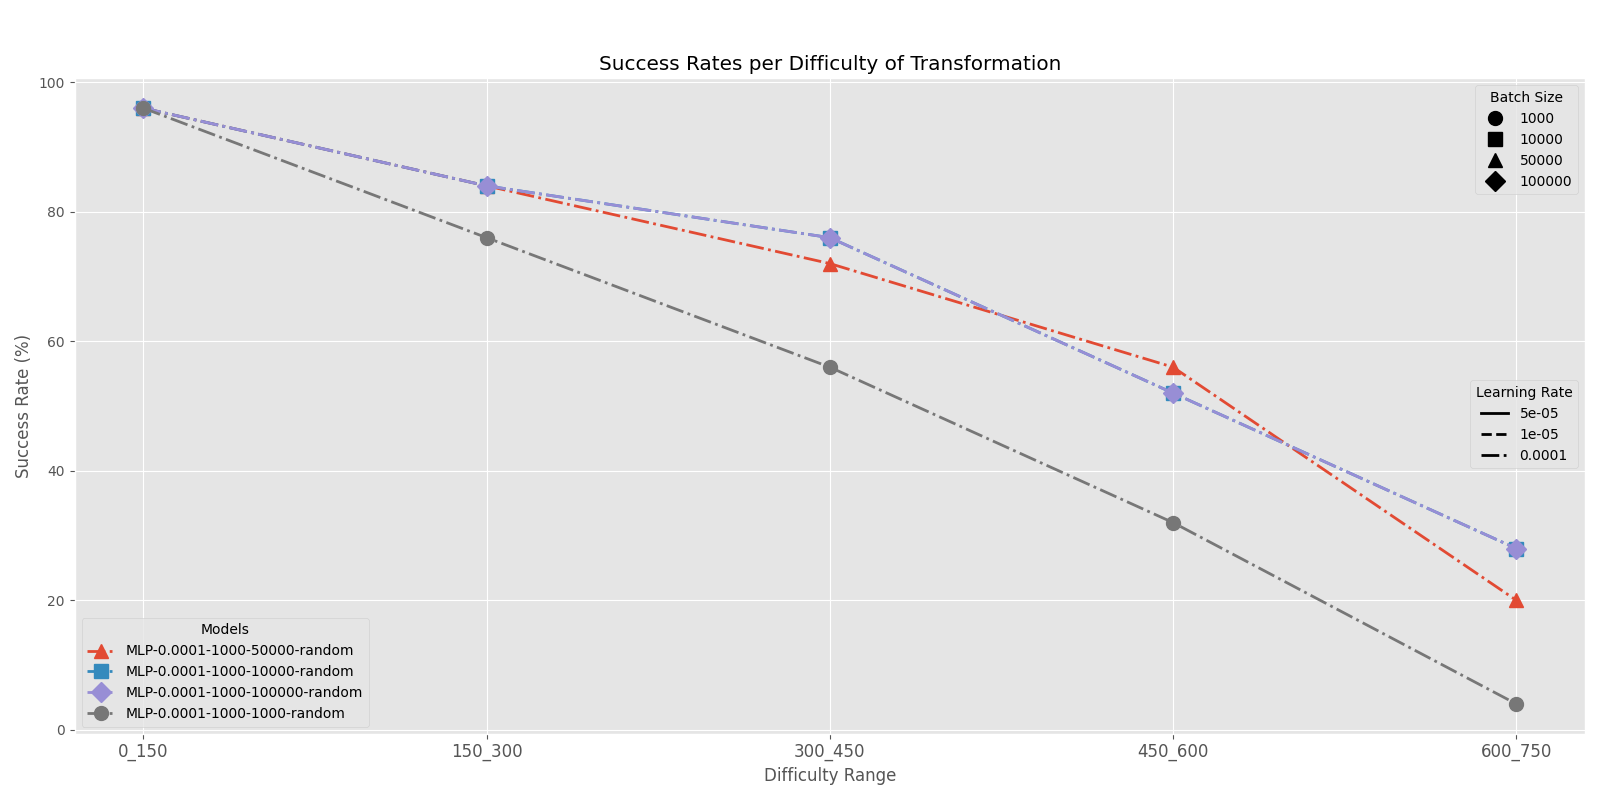
\includegraphics[width=0.8\textwidth]{imaxes/batchsize/experiment_plot_RFMID_MLP_0.0001.png}
%     \caption{Comparación do rendemento da rede con diferentes batch sizes sobre imaxes do dataset RFMID ca función de activación ReLU (learning rate = 1e-4)}
%     \label{fig:batch_size_comparison_relu_1e-4}
% \end{figure}

% \begin{figure}[tbp] 
%     \centering
%     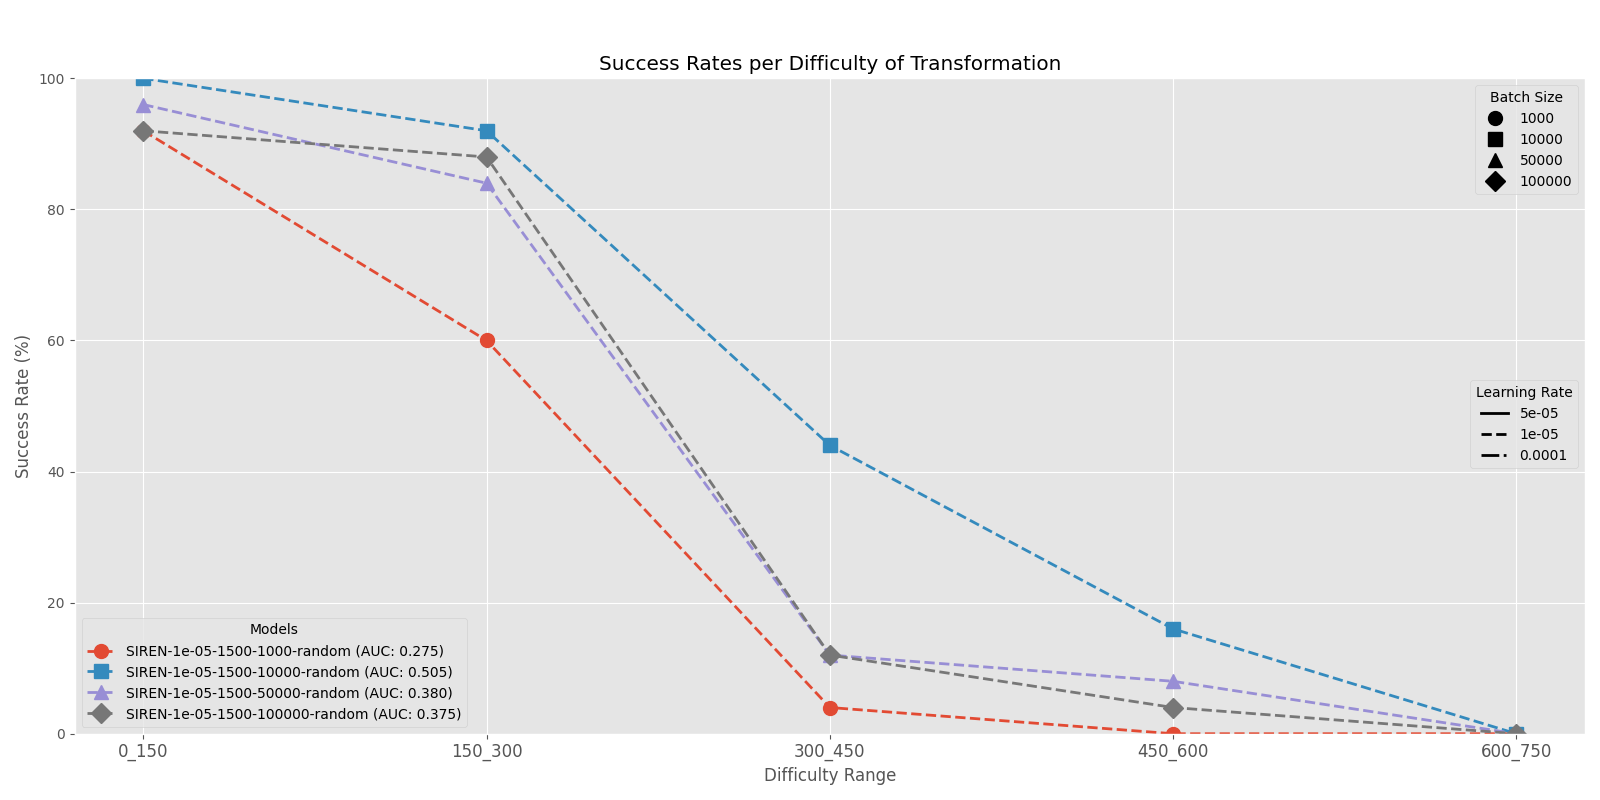
\includegraphics[width=0.8\textwidth]{imaxes/batchsize/experiment_plot_RFMID_SIREN_1e-05.png}
%     \caption{Comparación do rendemento da rede con diferentes batch sizes sobre imaxes do dataset RFMID ca función de activación SIREN (learning rate = 1e-5)}
%     \label{fig:batch_size_comparison_siren_1e-5}
% \end{figure}

% \begin{figure}[tbp] 
%     \centering
%     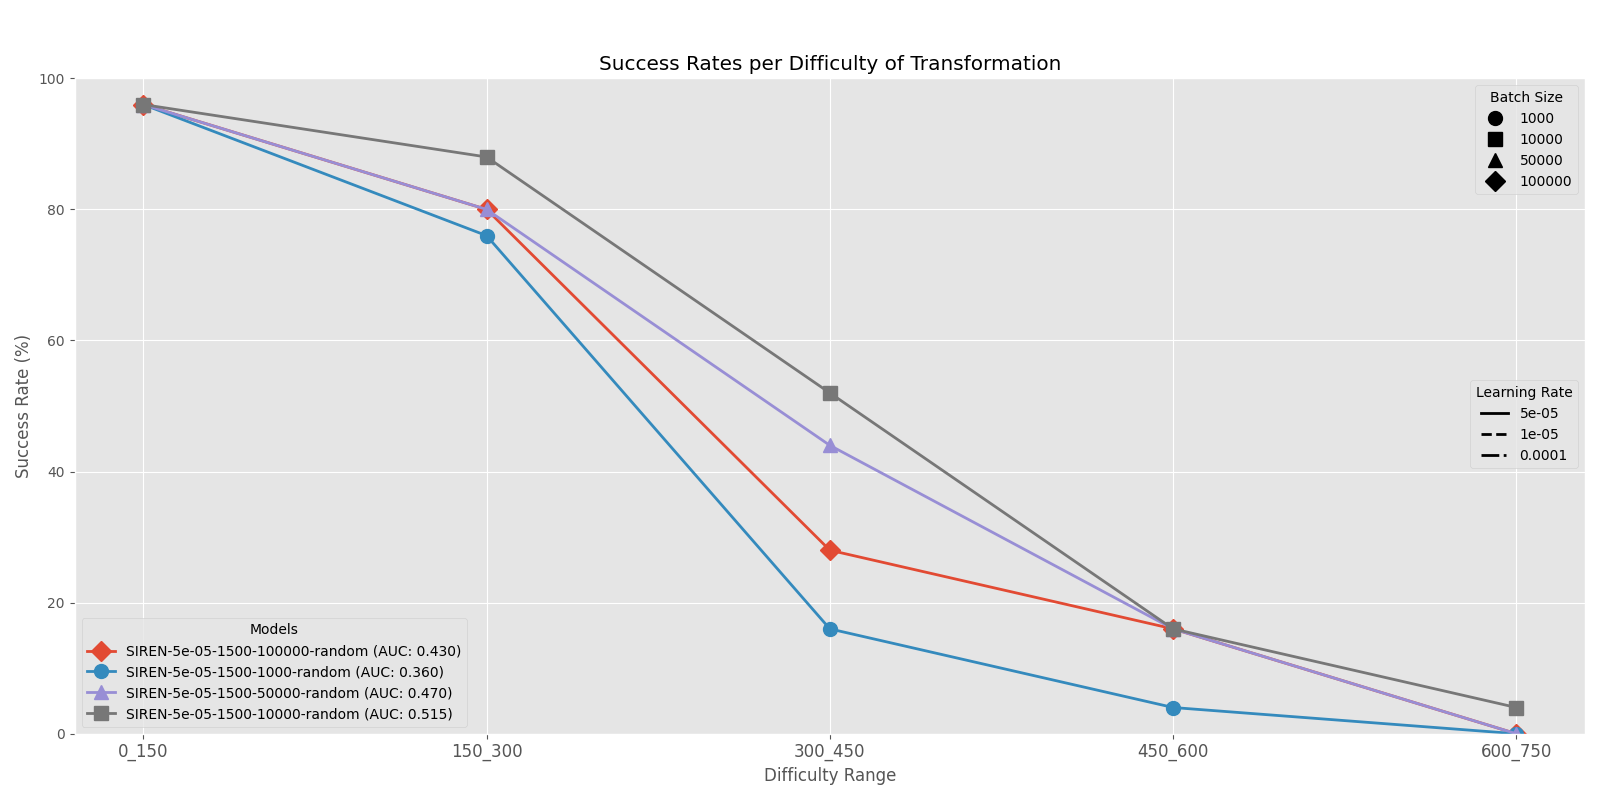
\includegraphics[width=0.8\textwidth]{imaxes/batchsize/experiment_plot_RFMID_SIREN_5e-05.png}
%     \caption{Comparación do rendemento da rede con diferentes batch sizes sobre imaxes do dataset RFMID ca función de activación SIREN (learning rate = 5e-5)}
%     \label{fig:batch_size_comparison_siren_5e-5}
% \end{figure}

% \begin{figure}[tbp] 
%     \centering
%     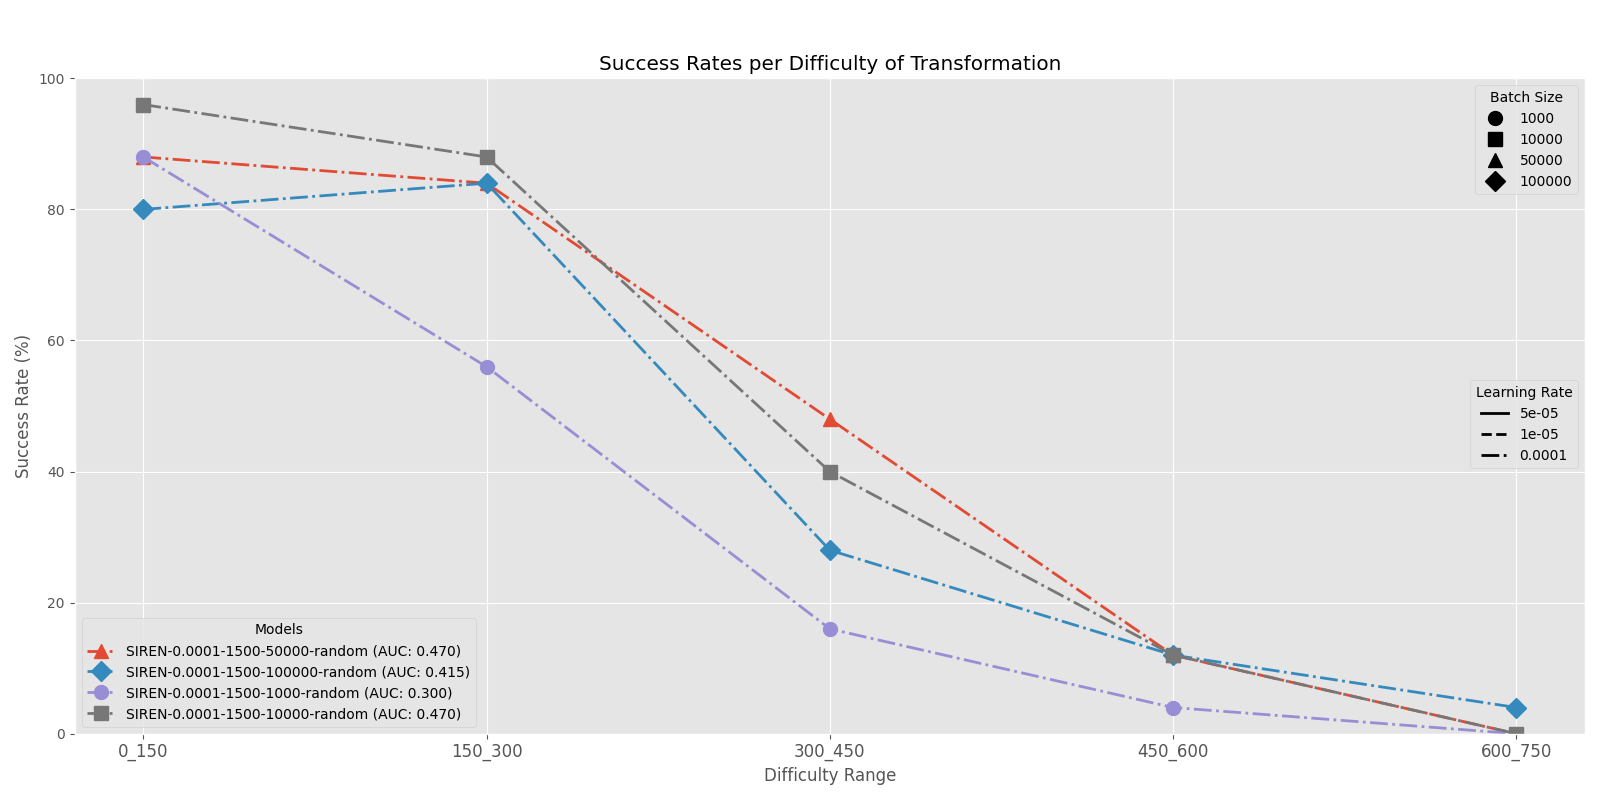
\includegraphics[width=0.8\textwidth]{imaxes/batchsize/experiment_plot_RFMID_SIREN_0.0001.png}
%     \caption{Comparación do rendemento da rede con diferentes batch sizes sobre imaxes do dataset RFMID ca función de activación SIREN (learning rate = 1e-4)}
%     \label{fig:batch_size_comparison_siren_1e-4}
% \end{figure}

% \FloatBarrier

\subsection{Discusión}
\label{subsec:Discusion-batchsize}

Obsérvase que as redes ca función de activación ReLU tenden a ter un rendemento moito mellor que as ca función de activación SIREN. Isto pode explicarse xa que as deformacións artificiais que se aplican nas imaxes do dataset RFMID son lineais, e a función de activación ReLU é adecuada para este tipo de transformacións.

Tamén parece que o tamaño de lote é relevante, especialmente o cambio entre 1000 e 10000, mentres que batch sizes maiores (50000, 100000) non parecen ter tanto impacto, aínda que si un maior custo computacional. 

Mentres que a rede é capaz de rexistrar correctamente consistentemente as imaxes do subconxunto mais sinxelos (0-150, 150-300), o rendemento decae notablemente para transformacións mais complexas (300+). 
Isto é mais notable cando se utiliza a función de activación SIREN, que ten dificultades incluso con transformacións de complexidade media, mentres que con ReLU decae de forma lineal.

\subsection{Conclusións}
\label{subsec:Conclusions-batchsize}

O principal factor limitador do rendemento da rede é o tamaño e complexidade das transformacións que tenta aprender.
Un tamaño de lote maior parece axudar, pero non é suficiente para rexistrar correctamente as imaxes con transformacións mais difíciles.

\section{Estratexias de mostraxe}
\label{sec:Estratexias de mostraxe}

Orixinalmente IDIR utiliza unha estratexia de mostraxe aleatoria para seleccionar os puntos que se pasan á rede en cada iteración.
Mentres que esta estratexia parece suficiente para o rexistro de pulmóns, no caso das imaxes de retina isto non ten porque ser así.
Isto débese a que as imaxes de retina conteñen seccións con moita mais información que outras, frente os CTs de pulmóns onde o sinal é mais uniforme.
Por exemplo, as seccións que conteñen vasos sanguíneos ou o disco óptico probablemente teñan mais información relevante para a tarefa de rexistro, frente outras seccións como o fondo da retina.
Ademais, as retinografías teñen desprazamentos moito maiores e menor superposición entre cada parella, polo que a rede ten que aprender transformacións mais complexas.

\subsection{Plantexamento}
\label{subsec:Plantexamento-sampling}

Plantexáronse novas estratexias de mostraxe, explicadas en detalle no apartado \ref{subsec:Metodoloxías Des}, cas cales preténdese mellorar o rendemento da rede ao proporcionarlle mais información relevante para a tarefa de rexistro.
As estratexias de mostraxe comparadas son as seguintes:
\begin{itemize}
    \item Mostraxe aleatoria: Selección aleatoria de puntos da imaxe.
    \item Mostraxe uniforme: Selección de puntos uniformemente espazados na imaxe. Especialmente relevante cando se usan batch sizes pequenos, xa que permite garantir que se amosan puntos de toda a imaxe.
    \item Mostraxe intelixente: Selección de puntos baseándose na información do gradiente da imaxe, priorizando as áreas con maior variación.
    \item Mostraxe ponderada: Punto intermedio entre a mostraxe aleatoria e a intelixente, onde se seleccionan puntos aleatoriamente pero con maior probabilidade nas áreas de maior interese.
\end{itemize}
% \FloatBarrier

\subsection{Resultados}
\label{subsec:Resultados-sampling}

Os resultados das diferentes estratexias de mostraxe sobre o dataset RFMID preséntanse na figura \ref{fig:sampling_types_comparisons}.

\begin{figure}[tbp]
    \centering
    \begin{subfigure}[b]{0.48\textwidth}
        \centering
        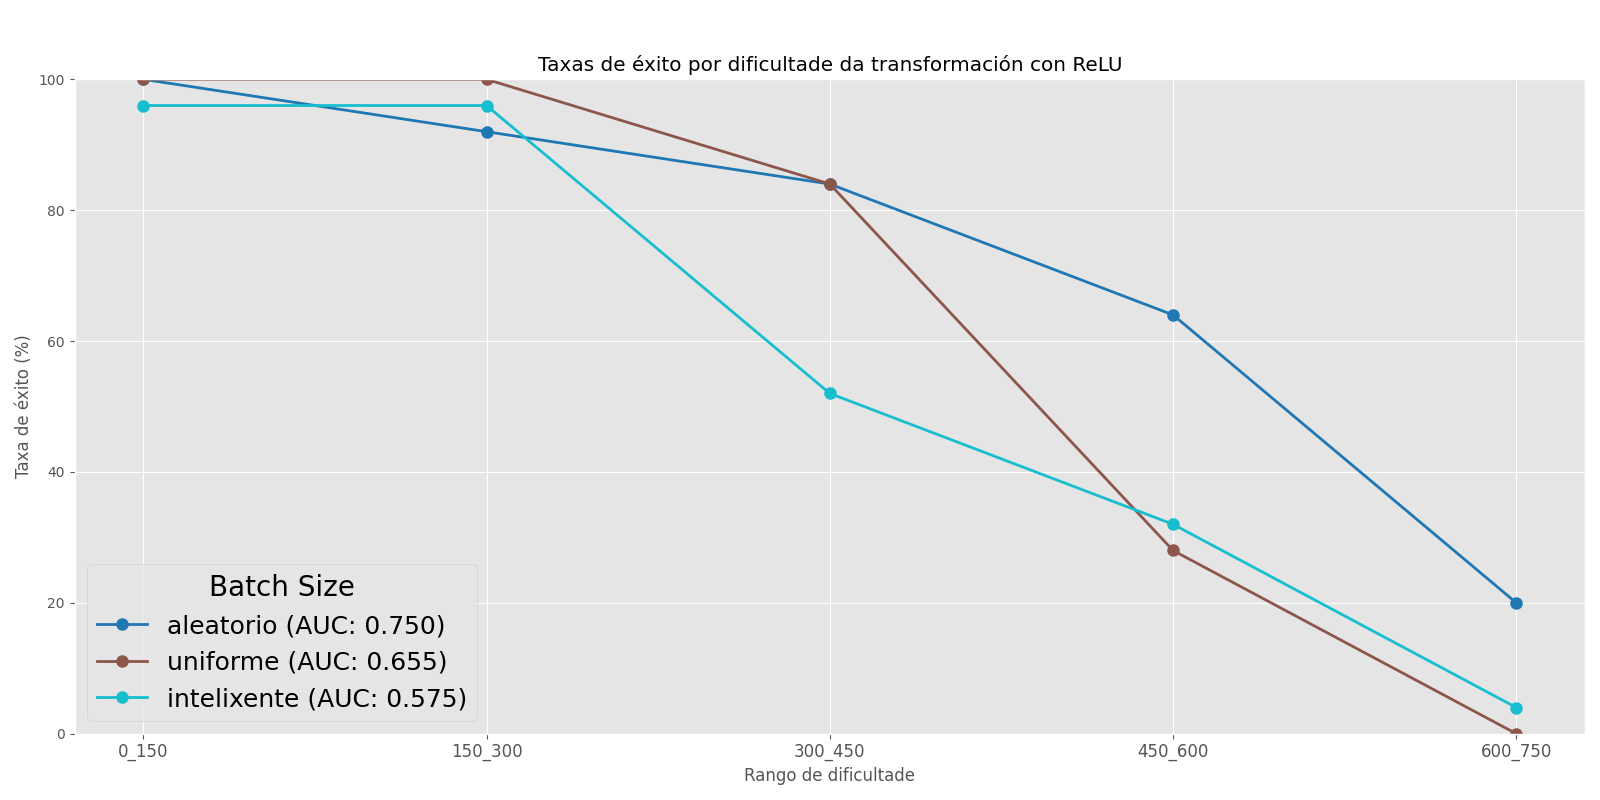
\includegraphics[width=\textwidth]{imaxes/muestraje/experiment_plot_RFMID_st_relu.png}
        \caption{Función de activación ReLU}
        \label{fig:sampling_types_relu}
    \end{subfigure}\hfill
    \begin{subfigure}[b]{0.48\textwidth}
        \centering
        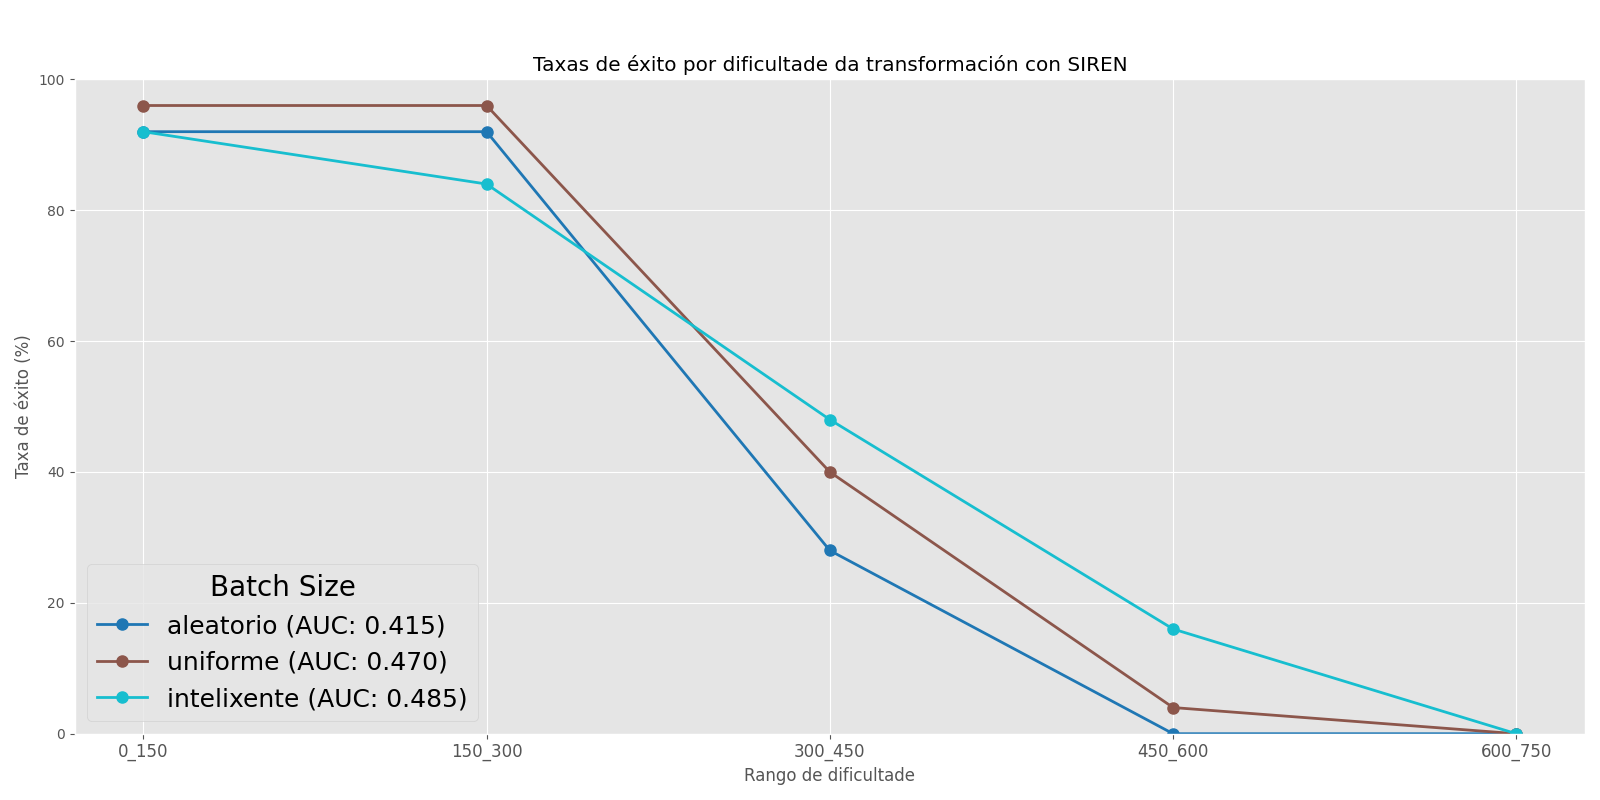
\includegraphics[width=\textwidth]{imaxes/muestraje/experiment_plot_RFMID_st_SIREN.png}
        \caption{Función de activación SIREN}
        \label{fig:sampling_types_siren}
    \end{subfigure}
    \caption{Comparación das diferentes estratexias de mostraxe sobre imaxes do dataset RFMID}
    \label{fig:sampling_types_comparisons}
\end{figure}



% \begin{figure}[tbp]
%     \centering
%     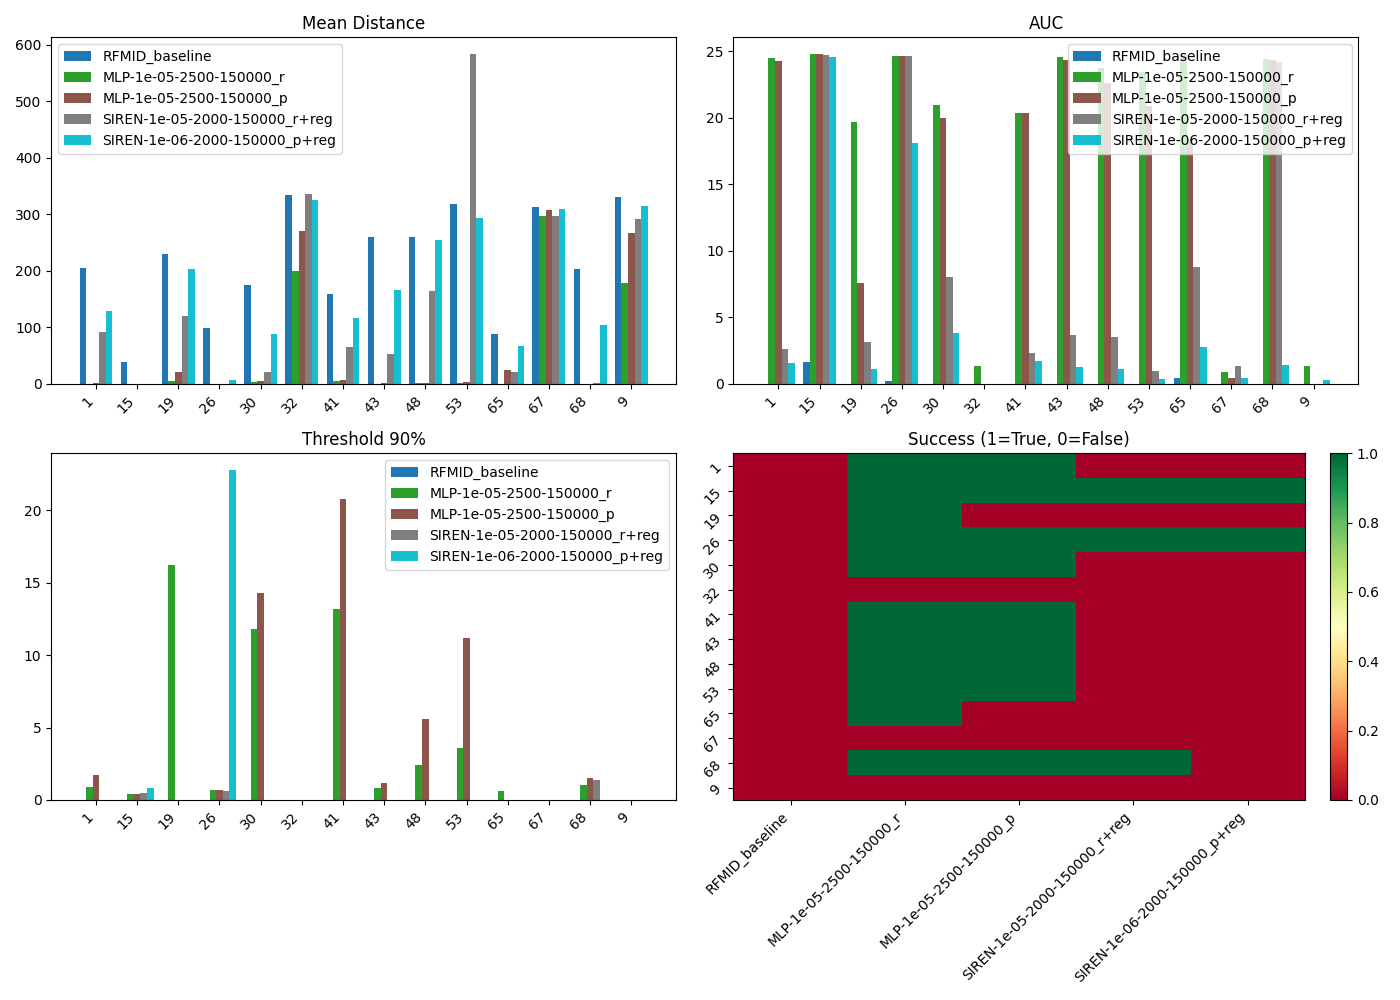
\includegraphics[width=0.8\textwidth]{imaxes/muestraje/RFMID_both__comp_sampling.png}
%     \caption{Comparación das diferentes estratexias de mostraxe sobre imaxes do dataset RFMID}
%     \label{fig:sampling_comparison}
% \end{figure}


% \ref{fig:fire_samplingtype}
% \ref{fig:sampling_comparison_relu}
% \ref{fig:sampling_comparison_SIREN}
% \begin{figure}[tbp]
%     \centering
%     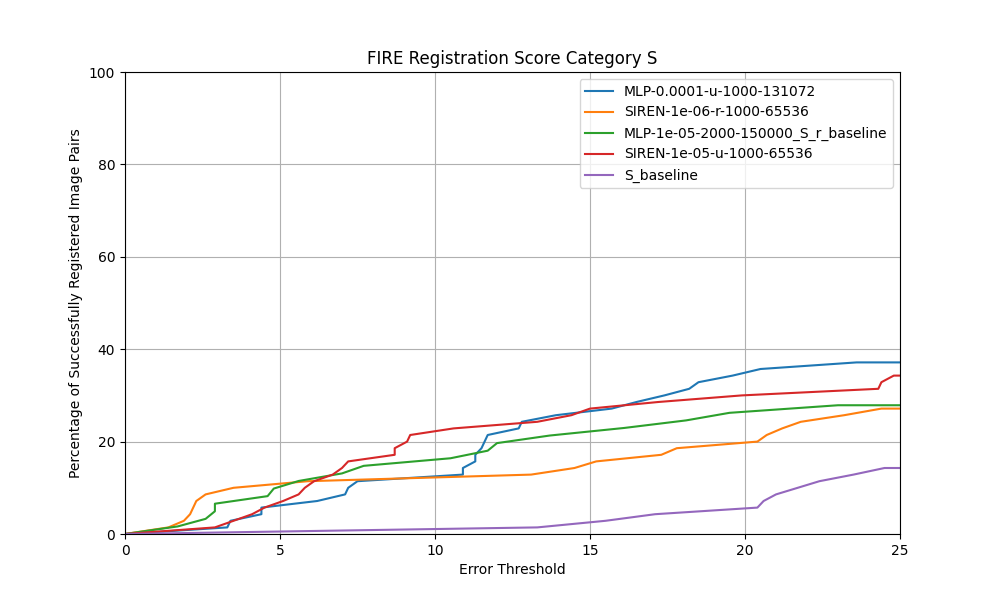
\includegraphics[width=0.8\textwidth]{imaxes/muestraje/fire_samplingtype.png}
%     \caption{Comparación das diferentes estratexias de mostraxe sobre imaxes do dataset FIRE}
%     \label{fig:fire_samplingtype}
% \end{figure}


% \begin{figure}[tbp]
%     \centering
%     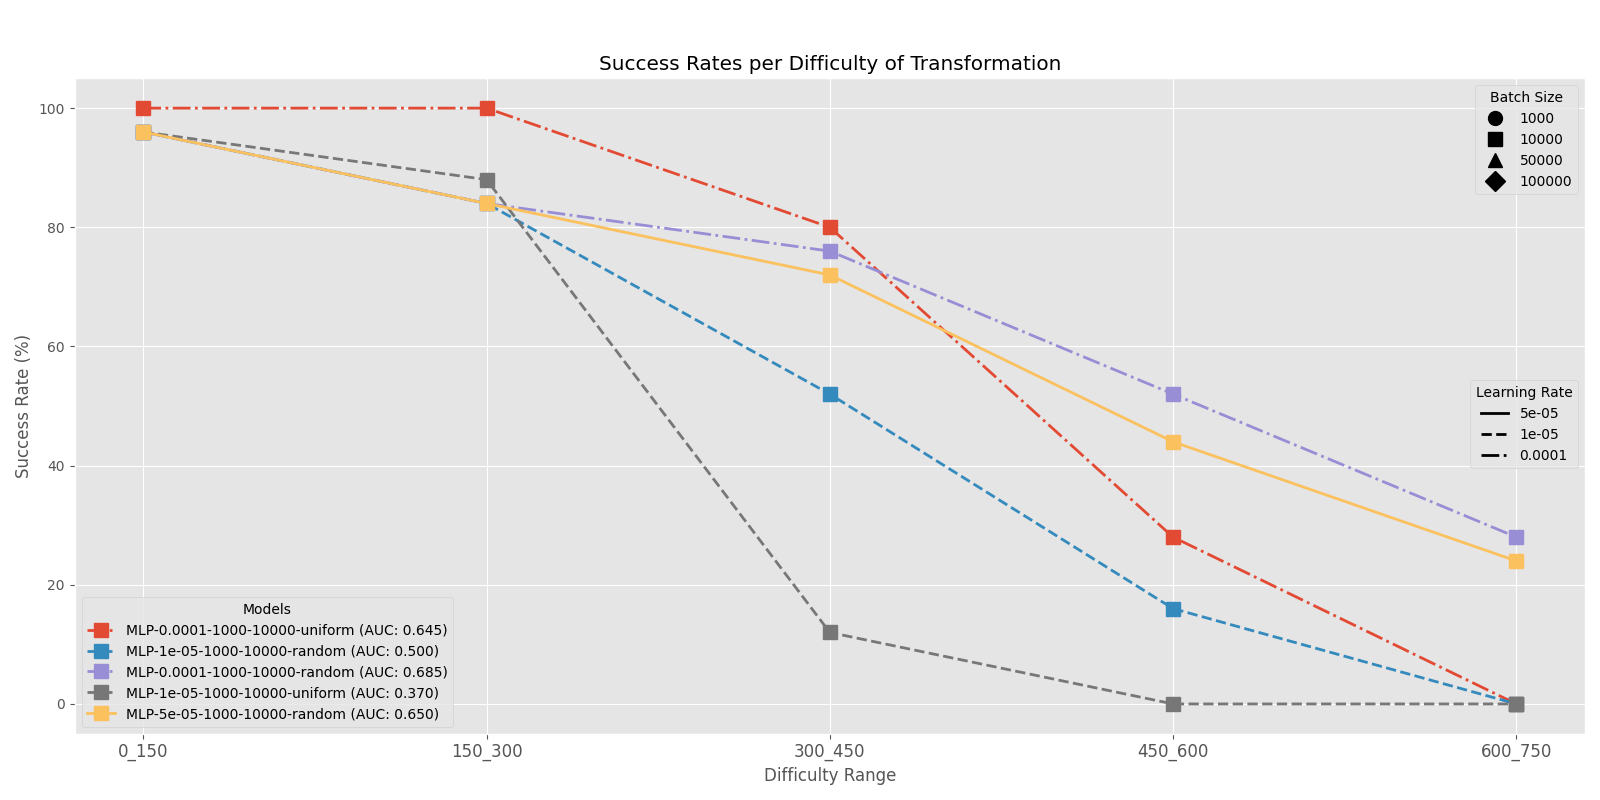
\includegraphics[width=0.8\textwidth]{imaxes/muestraje/experiment_plot_RFMID_MLP_RvsU.png}
%     \caption{Comparación das diferentes estratexias de mostraxe sobre imaxes do dataset RFMID ca función de activación RELU}
%     \label{fig:sampling_comparison_relu}
% \end{figure}

% \begin{figure}[tbp]
%     \centering
%     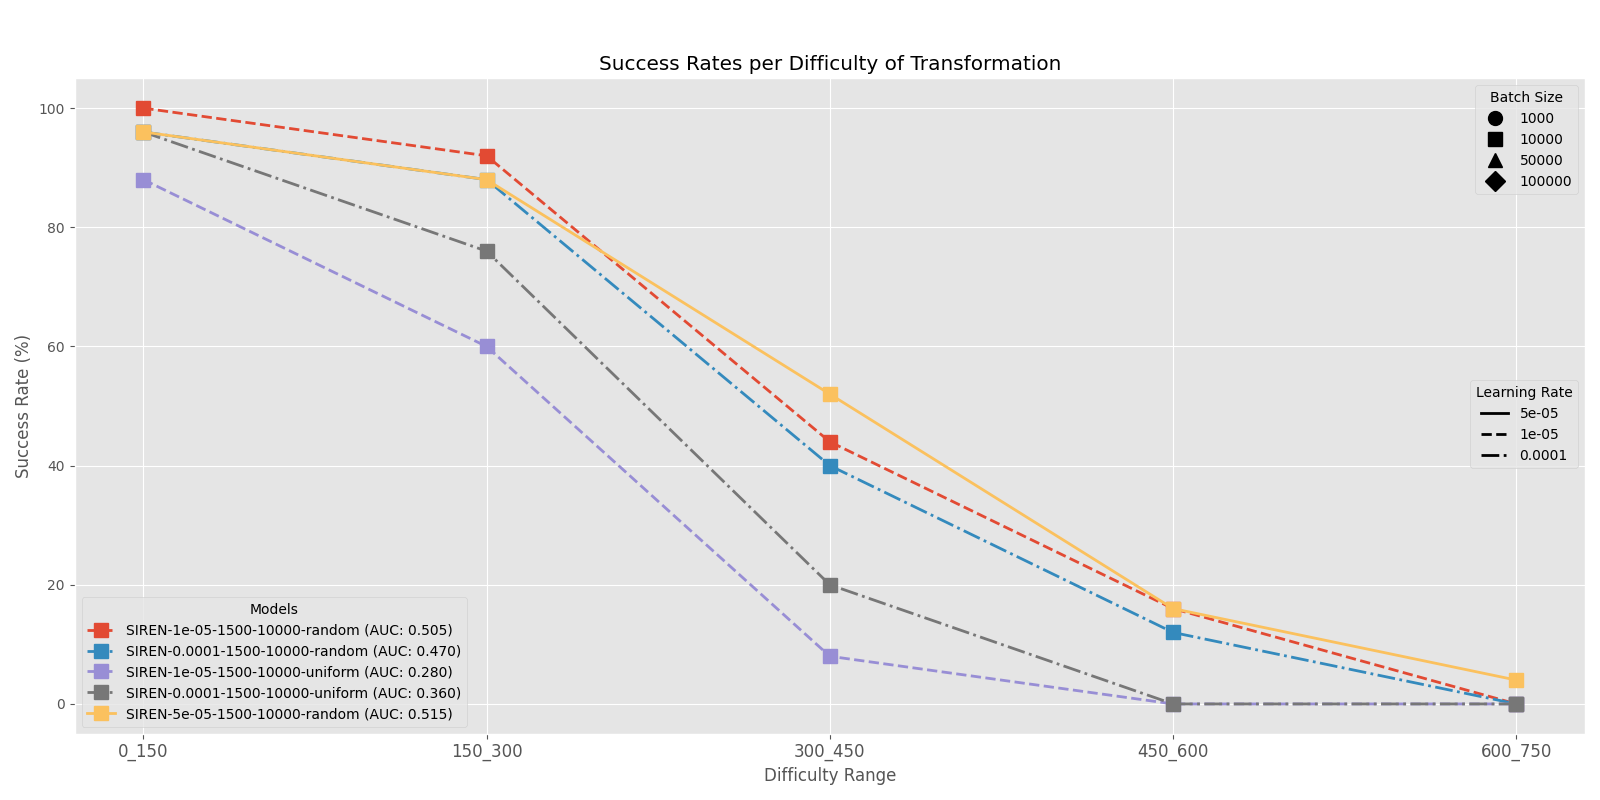
\includegraphics[width=0.8\textwidth]{imaxes/muestraje/experiment_plot_RFMID_SIREN_RvsU.png}
%     \caption{Comparación das diferentes estratexias de mostraxe sobre imaxes do dataset RFMID ca función de activación SIREN}
%     \label{fig:sampling_comparison_SIREN}
% \end{figure}


% \FloatBarrier

\subsection{Discusión}
\label{subsec:Discusion-sampling}

A hipótese da estratexia de mostraxe intelixente non parece ser axeitada, con resultados similares á estratexia aleatoria. 
O mesmo ocurre ca estratexia uniforme.

Igual que en experimentos anteriores, a función de activación ReLU parece dar mellores resultados que SIREN con RFMID, especialmente con maiores dificultades de transfomación.
% Non se experimentou con FIRE xa que os resultados iniciais non foron satisfactorios.

% \paragraph{Conclusións}
% \label{par:Conclusions-sampling}

\subsection{Conclusións}
\label{subsec:Conclusions-sampling}
Conclúese que, en contra da hipótese inicial, as estratexias de mostraxe implementadas, como a ponderada polo contido da imaxe, non aportan unha mellora significativa no rendemento do rexistro en comparación coa mostraxe aleatoria estándar. Isto suxire que a información relevante para a deformación está o suficientemente ben distribuída como para que unha mostraxe aleatoria sexa capaz de capturar os puntos necesarios para a converxencia, sempre que o tamaño de lote sexa adecuado.


\section{Inicialización}
\label{sec:Inicialización}

\subsection{Planteamento}
\label{subsec:Planteamento-initialization}

É posible que a inicialización da rede sexa un factor clave, e que certos desprazamentos iniciais provoque que que a rede sexa incapaz de aprender a transformación correcta, ou que lle custe moito mais aprenderla.

Para testar esta hipótese implementouse unha lotería de inicialización, onde se utiliza a perda na época 0 para determinar a inicialización da rede máis beneficiosa sobre a que seguir entrenando.

% \ref{fig:lottery_initial_deformations_combinedMLP}, \ref{fig:lottery_initial_deformations_combinedSIREN}

\begin{figure}[tbp]
    \centering
    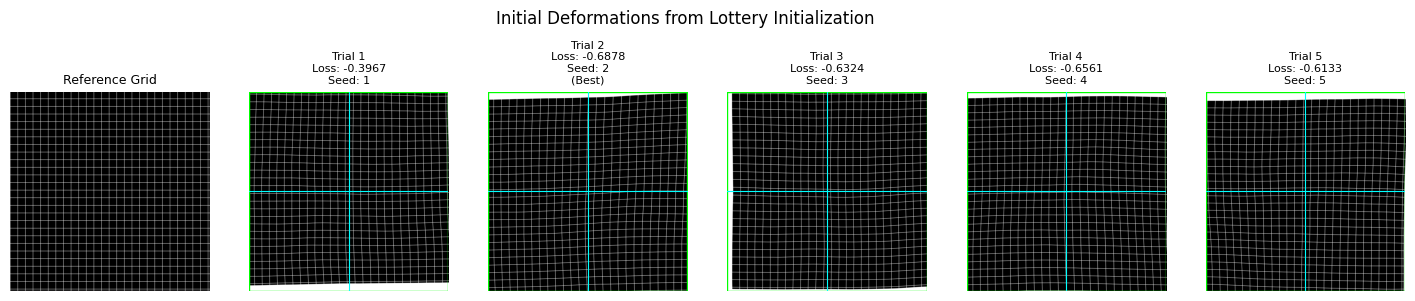
\includegraphics[width=0.8\textwidth]{imaxes/lottery/initial_deformations_combinedMLP.png}
    \caption{Exemplos das diferentes inicializacións ca función de activación RELU}
    \label{fig:lottery_initial_deformations_combinedMLP}
\end{figure}

\begin{figure}[tbp]
    \centering
    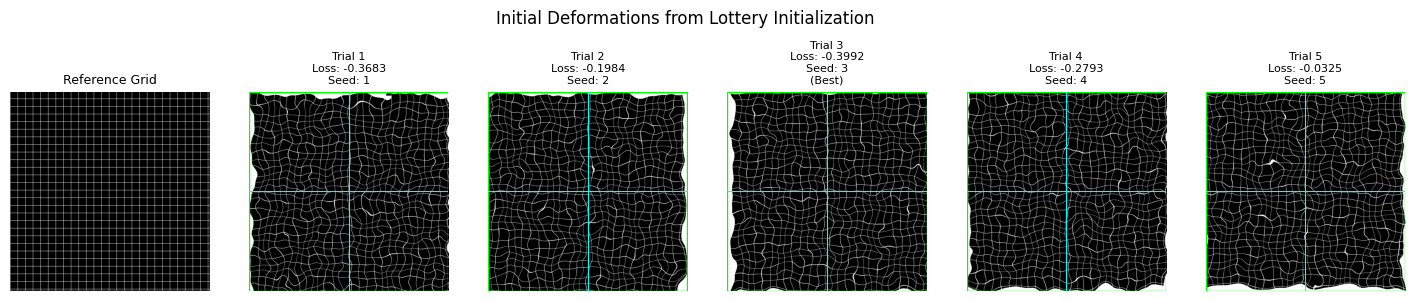
\includegraphics[width=0.8\textwidth]{imaxes/lottery/initial_deformations_combinedSIREN.png}
    \caption{Exemplos das diferentes inicializacións ca función de activación SIREN}
    \label{fig:lottery_initial_deformations_combinedSIREN}
\end{figure}

% \FloatBarrier

\subsection{Resultados}
\label{subsec:Resultados-initialization}


Na figura \ref{fig:lottery} amósanse os resultados de diferentes valores da lotería de inicialización.


\begin{figure}[tbp]
    \centering
    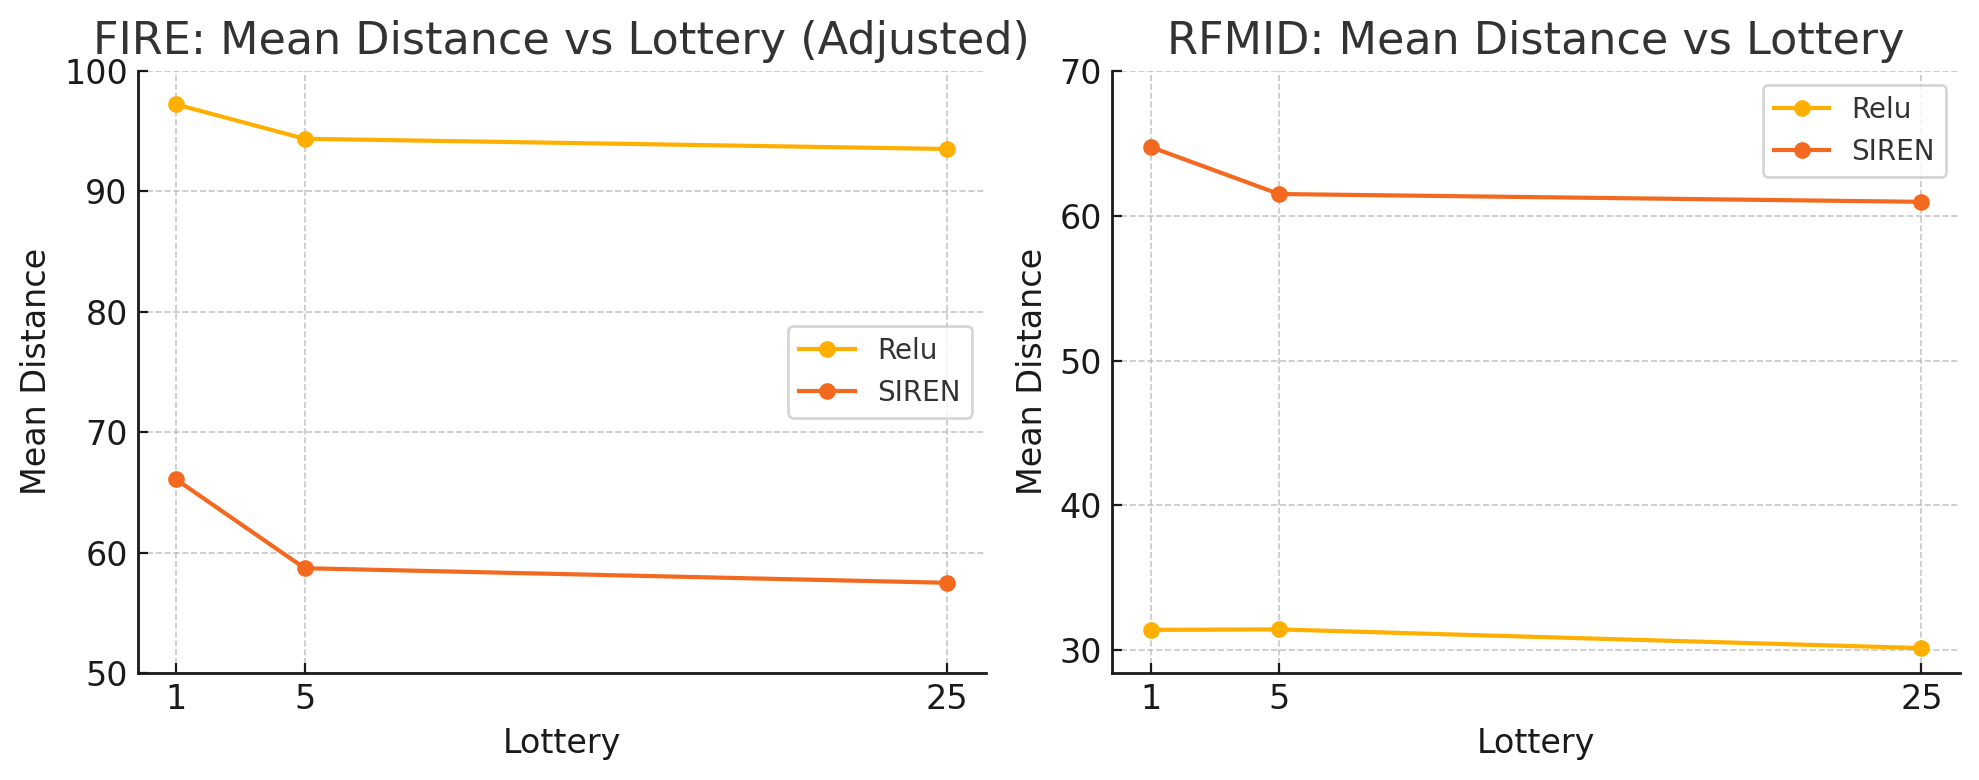
\includegraphics[width=0.8\textwidth]{imaxes/lottery/lotery.png}
    \caption{Resultados da lotería de inicialización}
    \label{fig:lottery}
\end{figure}

% \FloatBarrier

\subsection{Discusión}
\label{subsec:Discusion-initialization}

A inicialización estándar de SIREN proposta por Sitzmann et al. \cite{sitzmann2020implicitneuralrepresentationsperiodic} foi deseñado para tareas de reconstrucción de imaxes, e non necesariamente para regresión de campos de deformación.
Isto pode provocar que o proceso de optimización dedique moito tempo a contrarestar unha mala inicialización. 

\subsection{Conclusións}
\label{subsec:Conclusions-initialization}

Obsérvase que a lotería de inicialización si que provoca melloras no rendemento da rede, aínda que non moi significativas, e non se beneficia particularmente de utilizar mais de 5 inicializacións.
É posible que fose mellor esperar ata unha iteración algo mais avanzado para determinar a inicialización, xa que na época 0 non hai ningunha seguridade de que non sexa un mínimo local, pero isto tamén implicaría un maior custo computacional.

Unha posible mellora á lotería de inicialización sería utilizar un número maior de épocas antes de determinar a inicialización gañadora, xa que a perda inicial non é necesariamente representativo do rendemento final da rede.
Da mesma forma, sería interesante comparar diferentes estratexias de inicialización, como a inicialización gaussiana ou a inicialización uniforme, para determinar se algunha delas proporciona unha vantaxe significativa sobre a inicialización estándar de SIREN.

\section{Axuste dinámico do tamaño de lote}
\label{sec:Dynamic tamaño de lote}

\subsection{Planteamento}
\label{subsec:Planteamento-phases}

Teorízase que a rede pode beneficiarse de dividir o proceso de rexistro en diferentes fases, onde inicialmente utilízase un tamaño de lote reducido para aprender a transformación global, e posteriormente aumentase o tamaño de lote para aprender as transformacións locais.
Para isto utilizaremos a estratexia de mostraxe uniforme, que permite asegurar que se cubre toda a imaxe de ca mesma densidade, o que é mais importante con batch sizes pequenos. O learning rate modifícase de forma proporcional para manter a relación entre este e o tamaño de lote.

\subsection{Resultados}
\label{subsec:Resultados-phases}

Os resultados de utilizar diferentes números de fases pódense observar na figura \ref{fig:nphases}.
\begin{figure}[tbp]
    \centering
    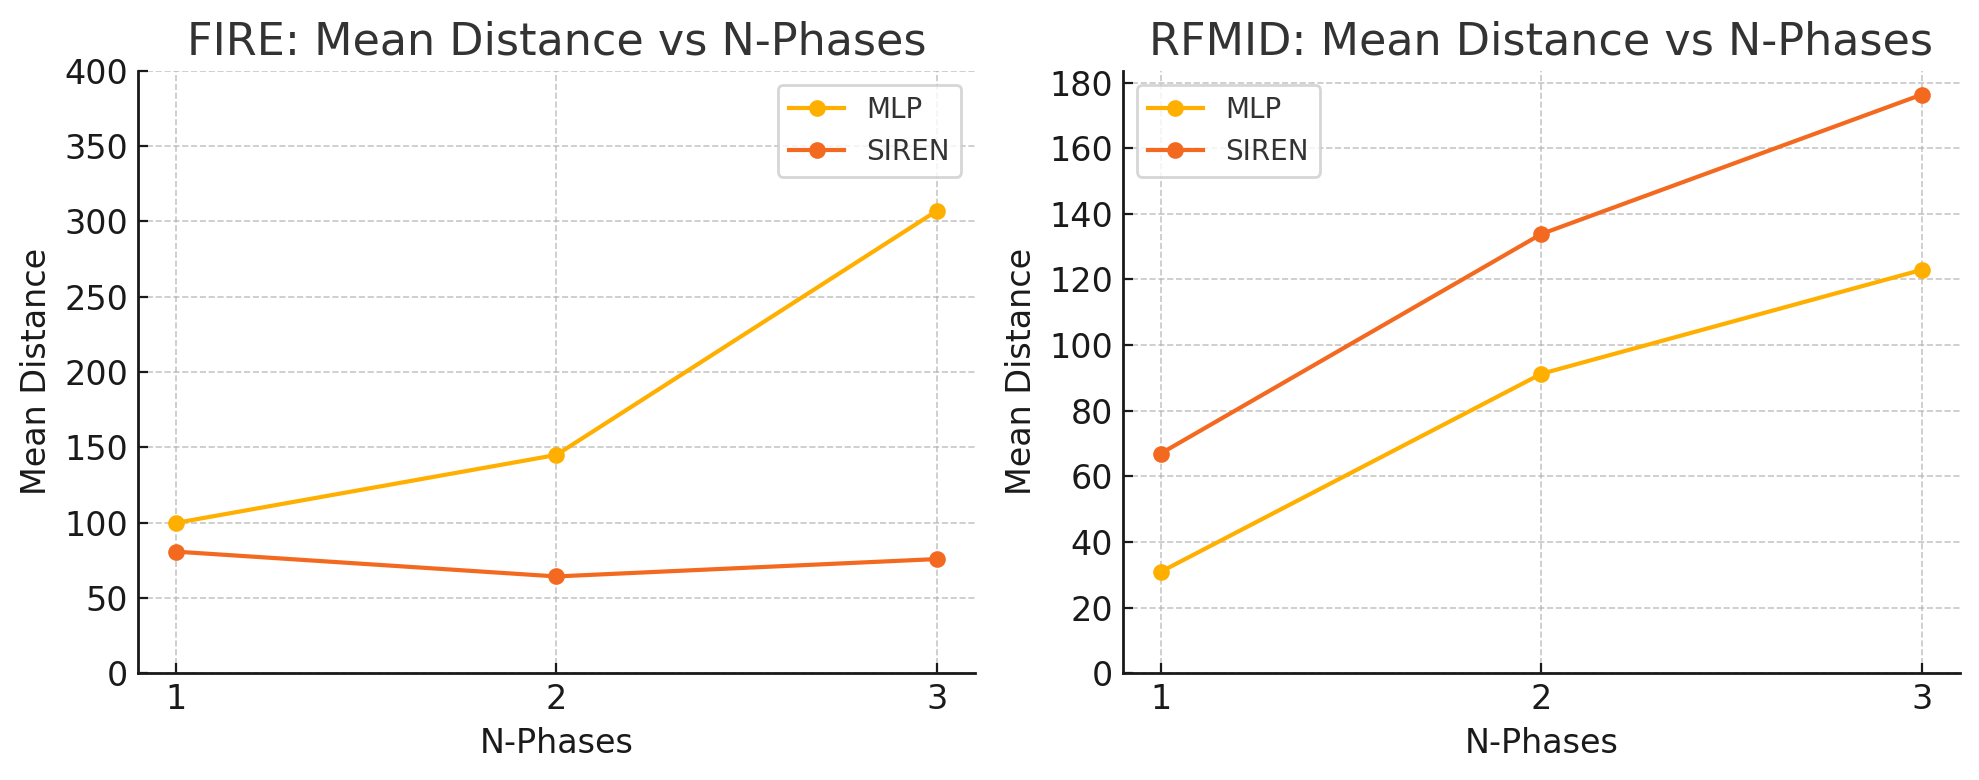
\includegraphics[width=0.8\textwidth]{imaxes/lottery/nphases.png}
    \caption{Resultados de usar distinto número de fases}
    \label{fig:nphases}
\end{figure}

% \FloatBarrier

\subsection{Discusión}
\label{subsec:Discusion-phases}

Os resultados presentados na figura \ref{fig:nphases} mostran unha tendencia clara e contraria á hipótese inicial, xa que o rendemento da rede empeora progresivamente a medida que se incrementa o número de fases. A estratexia de comezar cun tamaño de lote pequeno para aprender a transformación global antes de refinar os detalles cun tamaño de lote maior resulta ser contraproducente.

Unha posible explicación é que a idea de que un lote pequeno favorece a aprendizaxe global é incorrecta neste contexto. Un tamaño de lote reducido ofrece unha estimación moi ruidosa e pouco representativa, o que pode levar o adestramento por un camiño inestable e impedir que a rede converxa cara a unha boa solución global na fase inicial. En cambio, un tamaño de lote grande e constante, como se validou na sección \ref{sec:Tamaño de lote}, proporciona dende o principio información suficiente tanto a nivel global como local, permitindo que a rede aprenda ambas as transformacións simultaneamente de forma máis estable e eficaz.

Polo tanto, a estratexia de dividir o adestramento en fases non só non aporta beneficios, senón que resulta prexudicial ao introducir inestabilidade nas etapas cruciais da aprendizaxe. Este experimento reforza a conclusión de que un tamaño de lote grande é fundamental para o éxito do rexistro con esta metodoloxía.

\subsection{Conclusións}
\label{subsec:Conclusions-phases}

Conclúese que a estratexia de axuste dinámico do tamaño de lote é ineficaz e prexudicial para esta tarefa. A inestabilidade introducida nas fases iniciais do adestramento anula calquera posible beneficio teórico de aprender as transformacións por etapas. A rede demostra ser máis robusta e eficaz cando se adestra cun tamaño de lote grande e constante dende o principio, confirmando que este enfoque é superior para aprender simultaneamente as características globais e locais da deformación.

% \FloatBarrier

\section{Comparativa e resumo de resultados}
\label{sec:Comparativa e resumo}

Tras a realización dos experimentos descritos anteriormente, pódense extraer as seguintes conclusións:

\subsection{Rendemento por dataset}
\label{subsec:Rendemento por dataset}

\textbf{Dataset FIRE:} O rendemento no dataset FIRE, que contén imaxes reais de retina, é significativamente mais baixo que no dataset RFMID. A categoría P resulta imposible de rexistrar debido ao baixo grado de superposición (<75\%). As categorías S e A mostran taxas de éxito ao redor do 20\%, sendo a categoría S lixeiramente superior.

\textbf{Dataset RFMID:} O rendemento no dataset RFMID é considerablemente mellor, especialmente para transformacións de baixa complexidade (norma de Frobenius 0-150), onde se alcanza un éxito do case 100\%. O rendemento decae progresivamente ca complexidade da transformación. 
\subsection{Comparación de funcións de activación}
\label{subsec:Comparación de funcións de activación}

Os resultados mostran unha clara diferenciación entre as funcións de activación segundo o tipo de dataset:

\textbf{ReLU:} Mostra un rendemento superior no dataset RFMID, debido á súa capacidade natural para aprender transformacións lineais.

\textbf{SIREN:} Aínda que teoricamente máis adecuada para aprender transformacións complexas, ten dificultades para representalas adecuadamente. Tende a transformacións locais e pouco realistas e se non se regulariza adecuadamente, converxe a mínimos locais non desexados.

\subsection{Impacto dos parámetros principais}
\label{subsec:Impacto dos parámetros principais}

\textbf{Función de perda:} As métricas baseadas en características estruturais (NCC, SSIM) son superiores para imaxes reais con variabilidade de iluminación (FIRE), mentres que as métricas baseadas en píxeles (L1, MSE) son máis efectivas para imaxes sen variabilidade (RFMID).

\textbf{Regularización:} A regularización hiperelástica é a mais relevante para evitar deformacións non realistas. O valor óptimo depende da parexa de imaxes concreta a rexistrar. SIREN require valores máis altos que ReLU xa que ten unha maior tendencia ao sobreaxuste.

\textbf{Tamaño de lote:} Constitúe un dos parámetros máis críticos. Batch sizes maiores (10000-50000) proporcionan mellores resultados que batch sizes pequenos (1000), aínda que o beneficio decrece para valores moi altos (>50000).

\textbf{Resolución:} Non se observan beneficios significativos por encima de 1000×1000 píxeles, suxerindo que a información relevante para o rexistro xa está capturada en resolucións moderadas.

\subsection{Limitacións identificadas}
\label{subsec:Limitacións identificadas}

\textbf{Complexidade das transformacións:} O factor limitador principal é a complexidade das transformacións. Tanto ReLU como SIREN mostran dificultades ca transformacións de alta complexidade, independentemente da optimización de parámetros.

\textbf{Superposición de imaxes:} A baixa superposición entre imaxes (categoría P de FIRE) dificulta enormememtne o rexistro, suxerindo que as redes implícitas requiren un mínimo de información compartida.

\textbf{Estratexias de mostraxe:} Contrario ao esperado, as estratexias intelixentes de mostraxe (ponderadas por contido) non mostran beneficios sobre o mostraxe aleatorio, suxerindo que a información relevante está distribuída de forma máis uniforme do esperado.

\subsection{Conclusións xerais}
\label{subsec:Conclusións xerais}

A fase experimental deste traballo, centrada na adaptación e evaluación dun marco baseado en representación neuronais implícitas para a tarefa de rexistro de imaxes oftalmolóxicas,
demostra que as redes implícitas son aplicables ao rexistro de imaxes de retina, pero con limitacións importantes.
 O rendemento depende criticamente da complexidade das transformacións e do grado de superposición entre imaxes. Aínda que os resultados son prometedores para casos de complexidade baixa a moderada, o rexistro de imaxes ca transformacións complexas ou baixa superposición segue sendo un desafío que require investigación adicional.

Se ben o rendemento actual non é óptimo, as comparacións con outras metodoloxías de rexistro do estado da arte deben ter en conta que a maioría delas integran coñecemento específico do dominio frente ao método aquí presentado, que funciona de forma xeral aprendendo a partir dos pixel.
Isto suxire futuras liñas de investigación que combinen as vantaxes das redes implícitas con coñecementos específicos do dominio, como a anatomía da retina ou as características dos vasos sanguíneos, para mellorar o rendemento en rexistros complexos.
O análise das limitacións do modelo e exploración de diferentes estratexias proporcionan unha base sólida para futuras investigacións no campo. 